\chapter{Results and Discussion}
\label{chapter_results}

The time has come to present the final results of this thesis. As there are quite a few exciting measurements to be presented, the structure of this chapter is as follows. In the first section, a brief reminder of the motivation and methodology for this analysis are given to help with the digestion of the observables to be presented. The next section presents the final results as they are, with lengthy discussions about the trends for each observable. The final sections will compare these results to theoretical models and previous measurements, and will discuss the implications of these measurements on the current understanding of strangeness production in heavy-ion collisions.


\section{Quick recap: motivation and methodology}

This section serves as a \textit{brief} recap of the ``how'' and ``why'' for this thesis. For more details, please refer to Chapter~\ref{ch:analysis_mnm}.

The goal of this thesis is to measure the production of strangeness (\lmb baryons) both in and out-of jets in \pPb collisions. By separating the production of $\Lambda$s in these regions, the underlying processes responsible for strangeness enhancement may be brought to light.

To perform this separation, \textbf{two-particle h-\lmb angular correlations} are used. Using these angular correlations with a high momentum trigger hadron, the production of $\Lambda$s can be separated into three regions: the near-side region (corresponding to unmodified jet-like production), the away-side region (corresponding to jet-like production with medium modification), and the underlying event or UE region (associated with soft production in the QGP medium). A diagram highlighting these regions can be seen in Figure~\ref{fig:dphi_cartoon_ref}.

\begin{figure}[h]
\centering
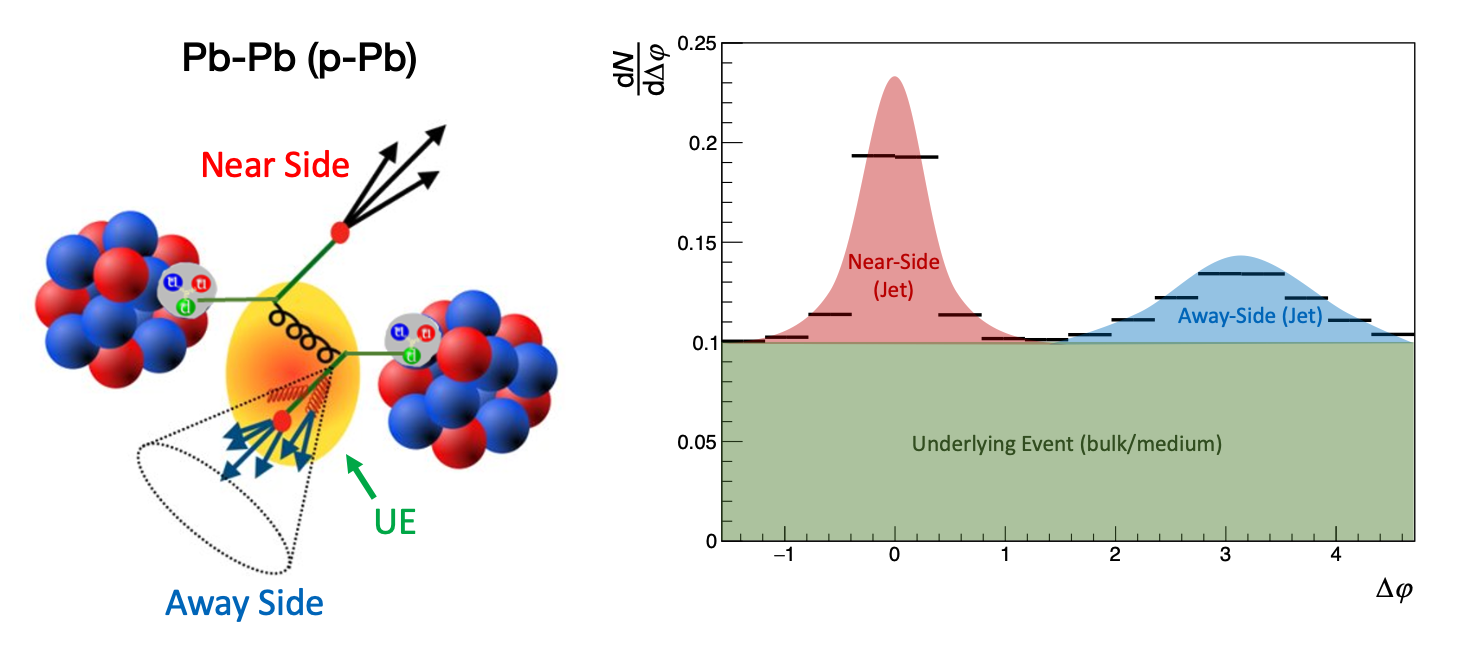
\includegraphics[width=\textwidth]{figures/mnm/dphi_cartoon.png}
\caption{A cartoon of a Pb--Pb (p--Pb) collision that produces particles in the near- and away-side jets, along with the UE. The the corresponding regions in the $\Delta\varphi$ distribution are highlighted on the right.}
\label{fig:dphi_cartoon_ref}
\end{figure}

The yields and widths presented in this section are extracted from these correlation distributions, and studied as a function of multiplicity and \lmb momentum. The same procedure is performed for charged hadrons (h-h), and the results are compared. These observables are also compared to multiple theoretical model predictions, as well as to similar results from the $\phi(1020)$ meson.

\section{Per-trigger $\Delta\varphi$ distributions}

The per-trigger h-h and h-\lmb $\Delta\varphi$ distributions for all multiplicity and associated \pt bins can be seen in Figure~\ref{fig:h_lambda_1d_final} (h-\lmb) and Figure~\ref{fig:h_h_1d_final} (h-h). Summarizing plots that contain both the h-\lmb and h-h distributions together for each multiplicity class for the lower ($1.5 <$ \pt $< 2.5$ \GeVc) and higher ($2.5 < $ \pt $< 4.0$ \GeVc) associated \pt bins can be seen in Figures \ref{fig:dphi_final_lowpt} and \ref{fig:dphi_final_highpt}, respectively. In the summarizing plots, the entire range along the y-axis is shown to emphasize the relative contribution to each distribution from the UE. 

In the lower associated momentum range, the UE baseline for both the h-\lmb and h-h distributions is found to increase by around a factor of three from the lowest to highest multiplicity class (0.05 to 0.17 in the h-\lmb case, 0.35 to 1 in the dihadron case). The higher associated momentum range exhibits a similar increase in the UE baseline with increasing multiplicity, but the h-\lmb baseline increases by a factor of four instead of three. The UE baseline is also found to be higher in the lower associated \pt range than in the higher range by around a factor of three in the h-\lmb case and four in the h-h case for each multiplicity class. These observations suggest that associated production in the UE region truly is ``softer'' than production in the near- and away-side regions, supporting the idea that the production in the UE is heavily linked to the QGP.

\begin{figure}[ht]
	\centering
	\begin{minipage}{0.48\textwidth}
		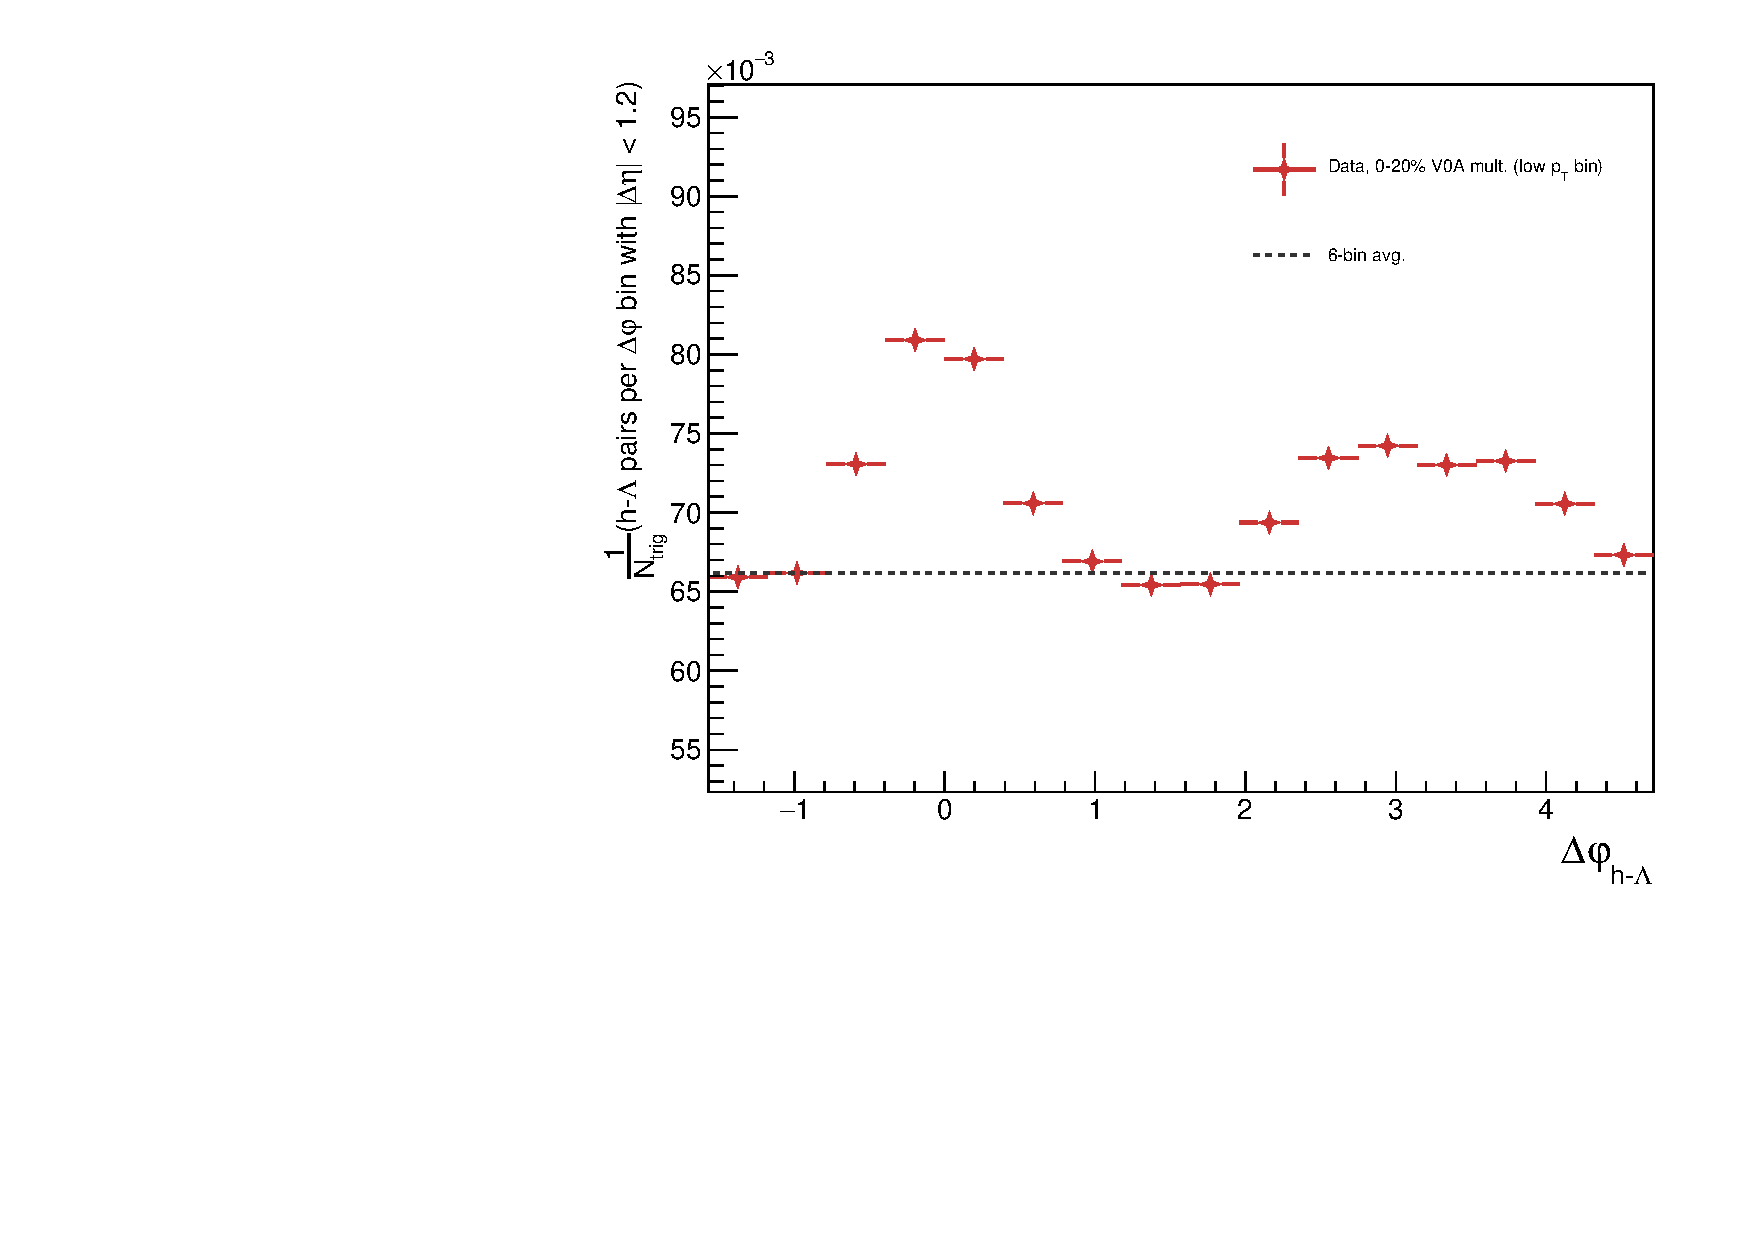
\includegraphics[width=\textwidth]{figures/analysis/h_lambda_dphi_avg6_0_20_lowpt.pdf}
	\end{minipage}
	\begin{minipage}{0.48\textwidth}
		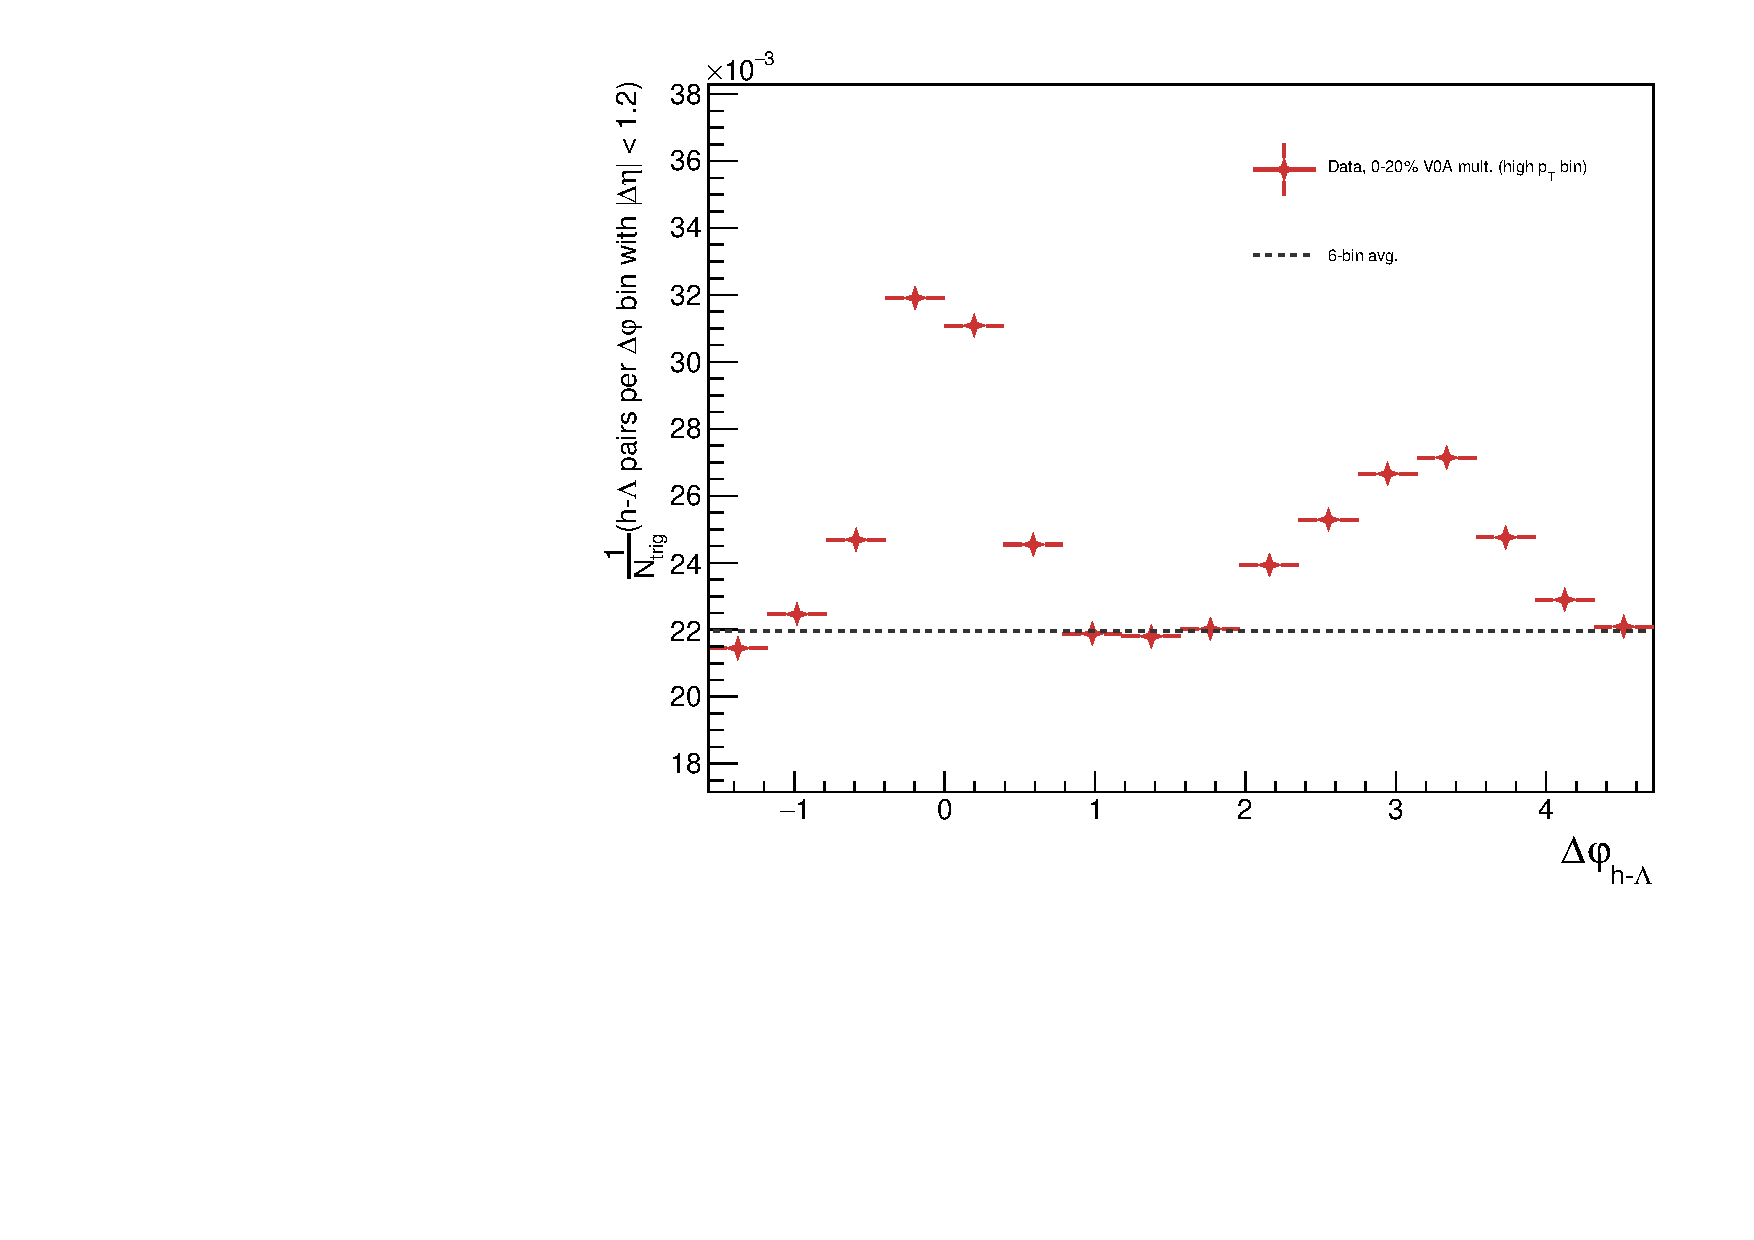
\includegraphics[width=\textwidth]{figures/analysis/h_lambda_dphi_avg6_0_20_highpt.pdf}
	\end{minipage}
	\begin{minipage}{0.48\textwidth}
		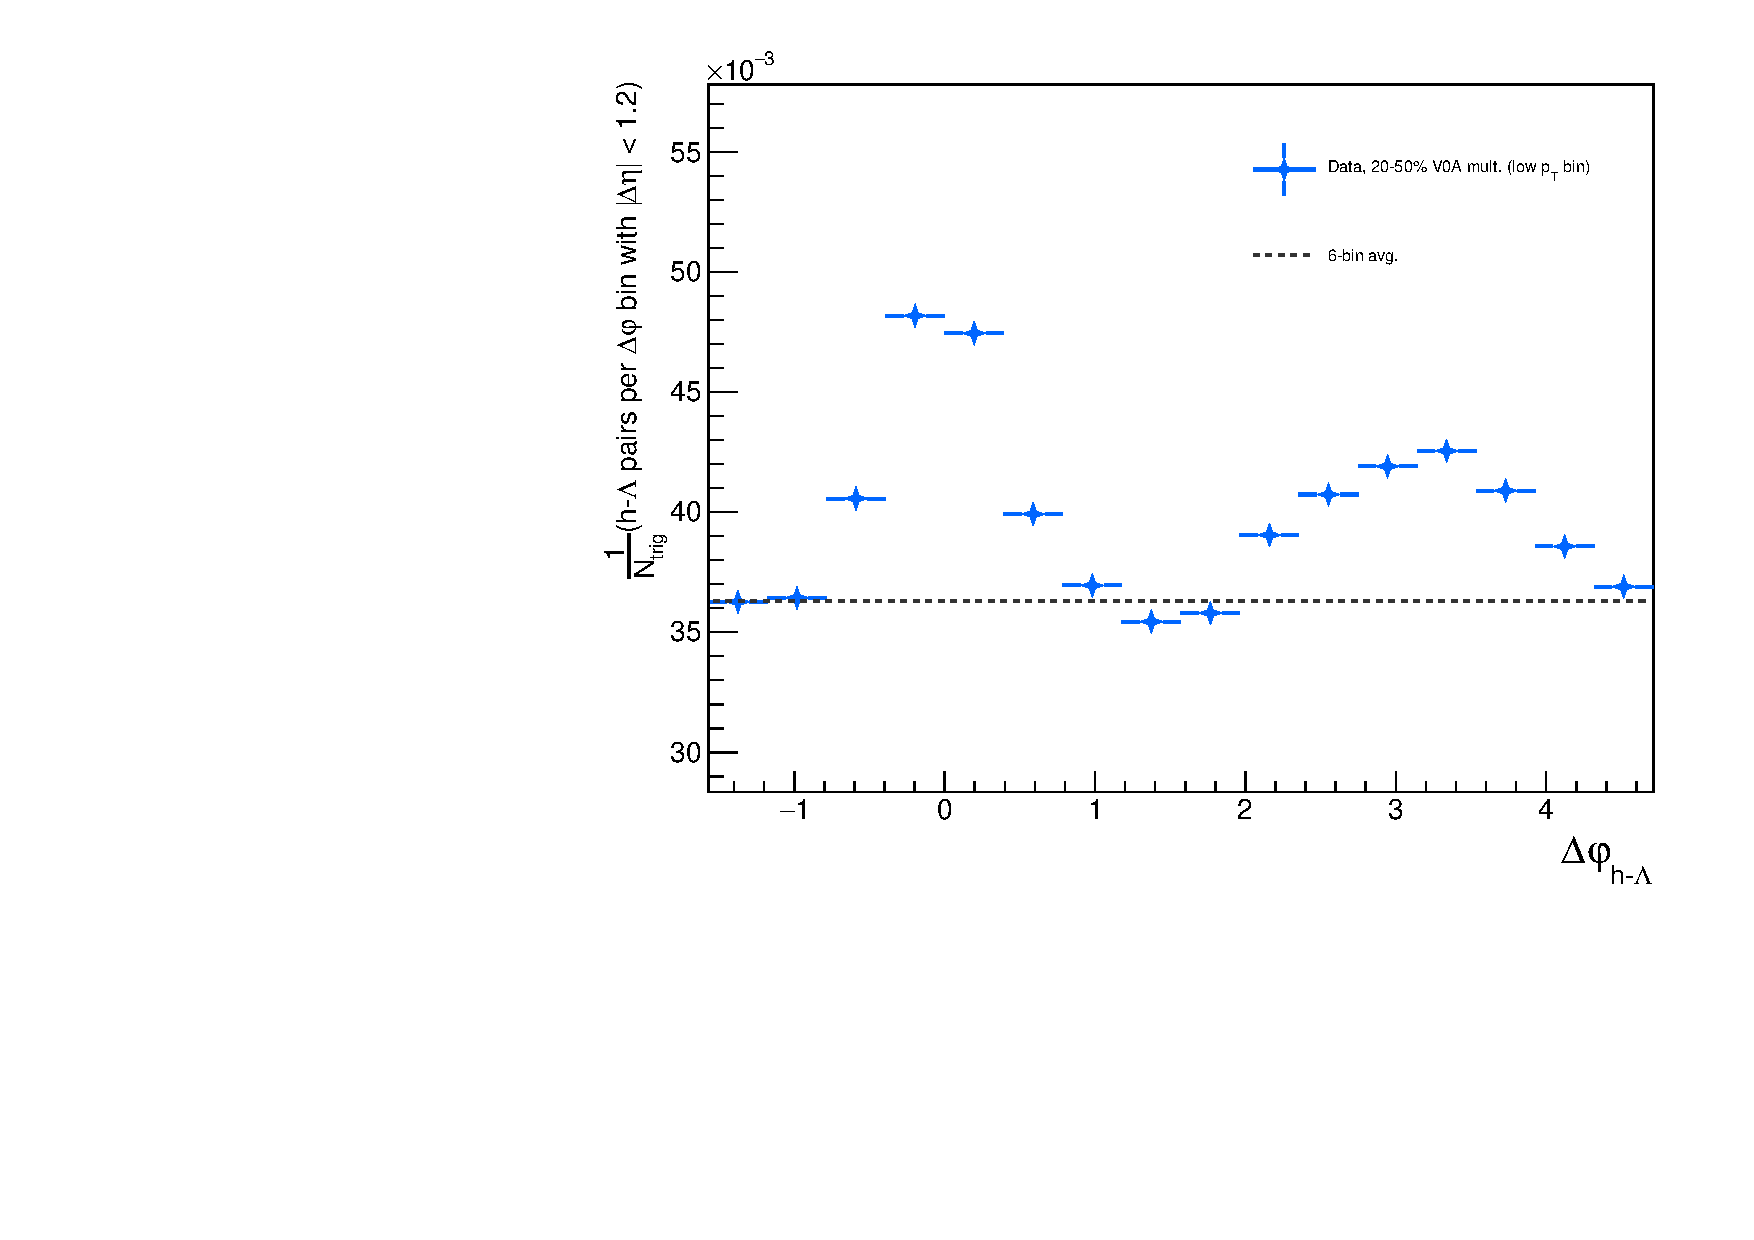
\includegraphics[width=\textwidth]{figures/analysis/h_lambda_dphi_avg6_20_50_lowpt.pdf}
	\end{minipage}
	\begin{minipage}{0.48\textwidth}
		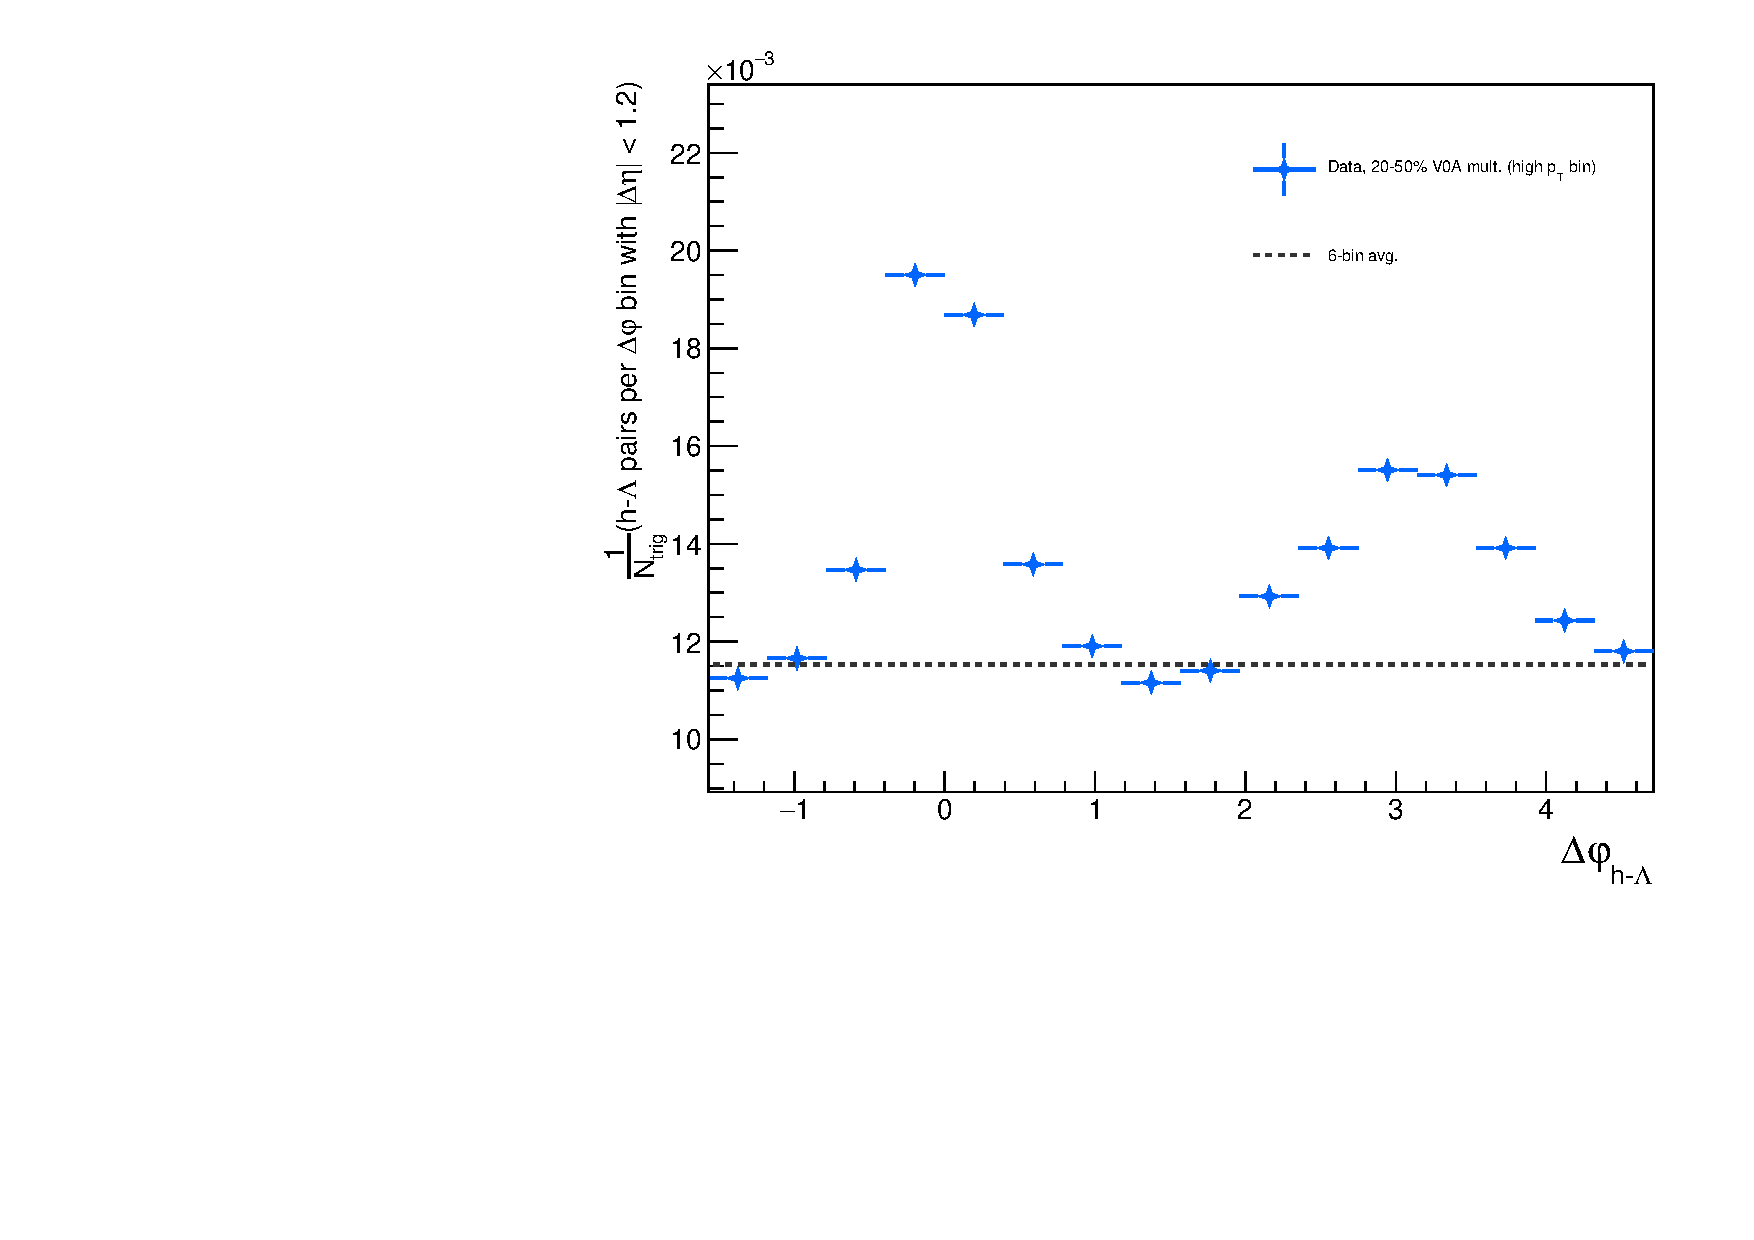
\includegraphics[width=\textwidth]{figures/analysis/h_lambda_dphi_avg6_20_50_highpt.pdf}
	\end{minipage}
	\begin{minipage}{0.48\textwidth}
		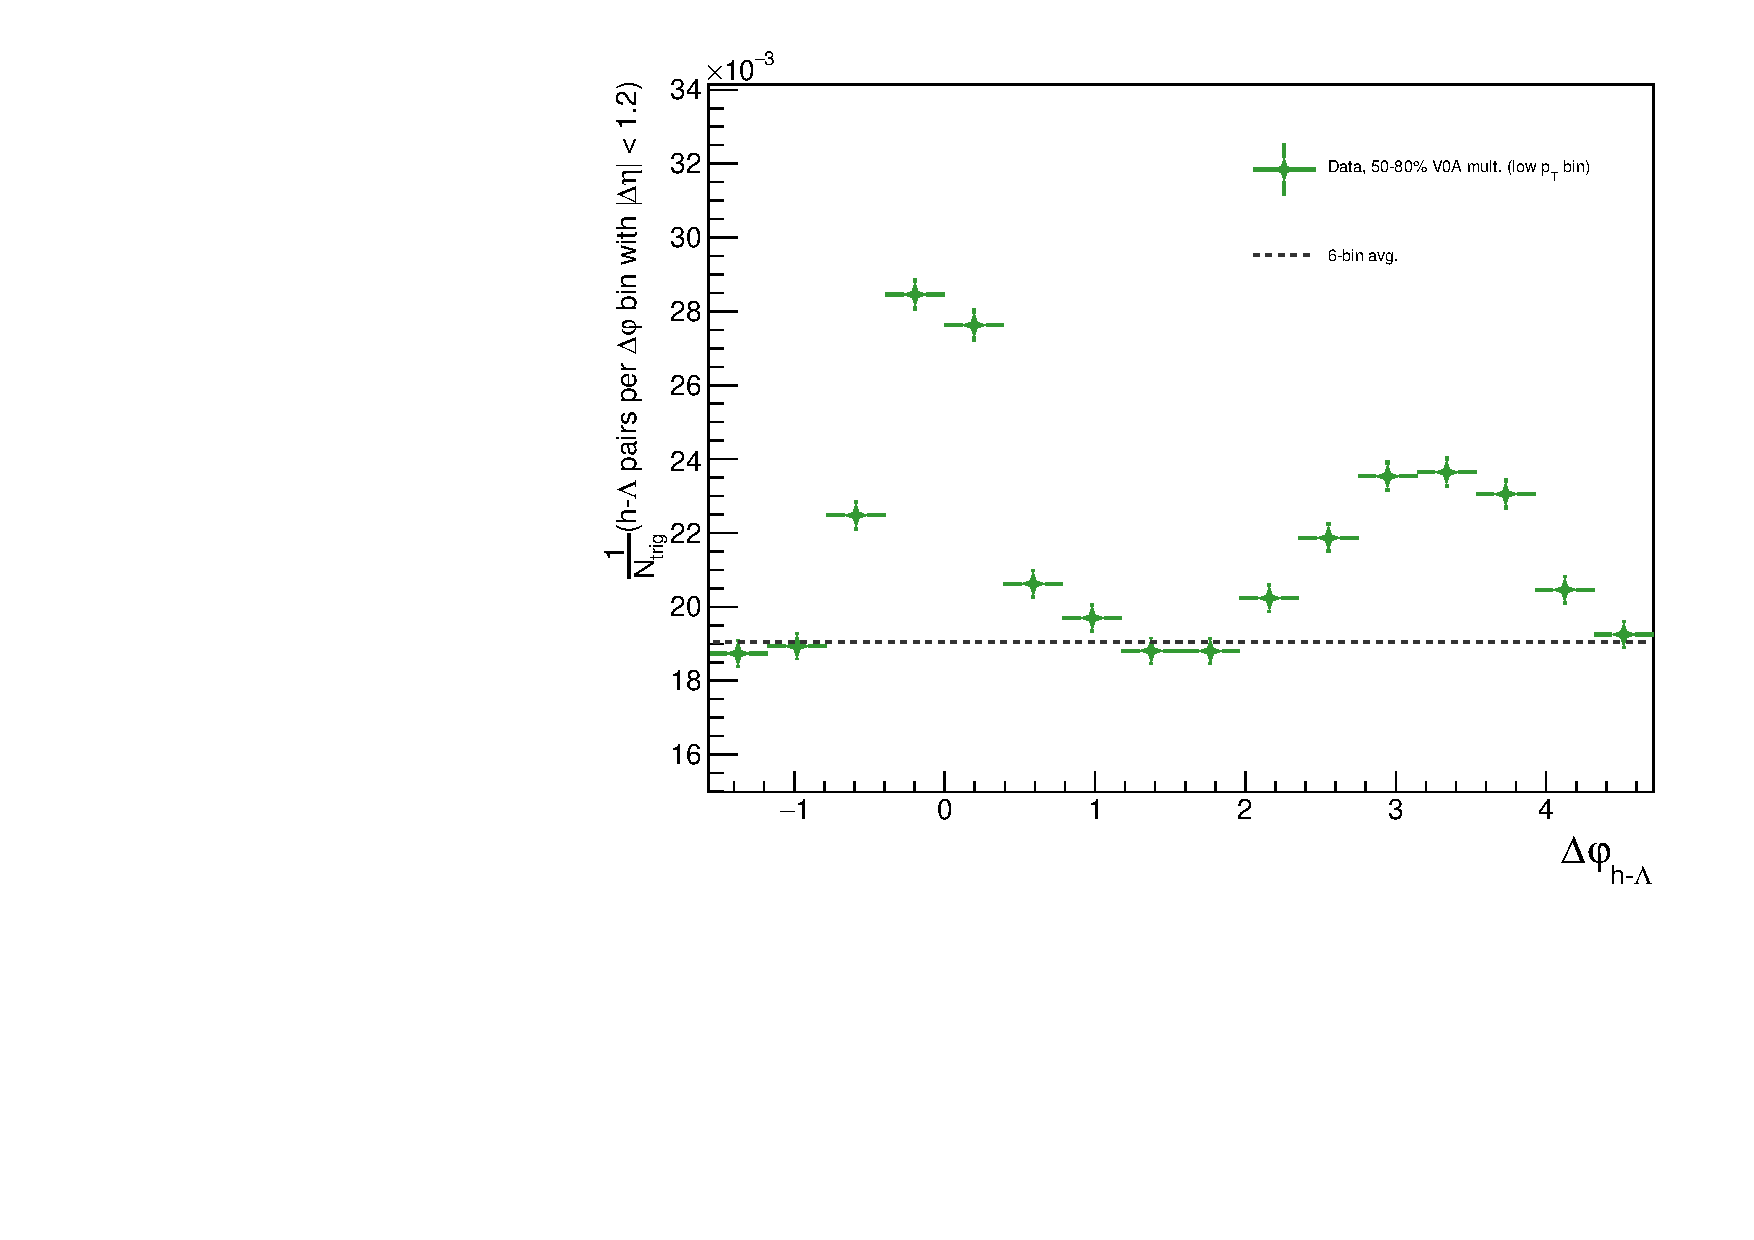
\includegraphics[width=\textwidth]{figures/analysis/h_lambda_dphi_avg6_50_80_lowpt.pdf}
	\end{minipage}
	\begin{minipage}{0.48\textwidth}
		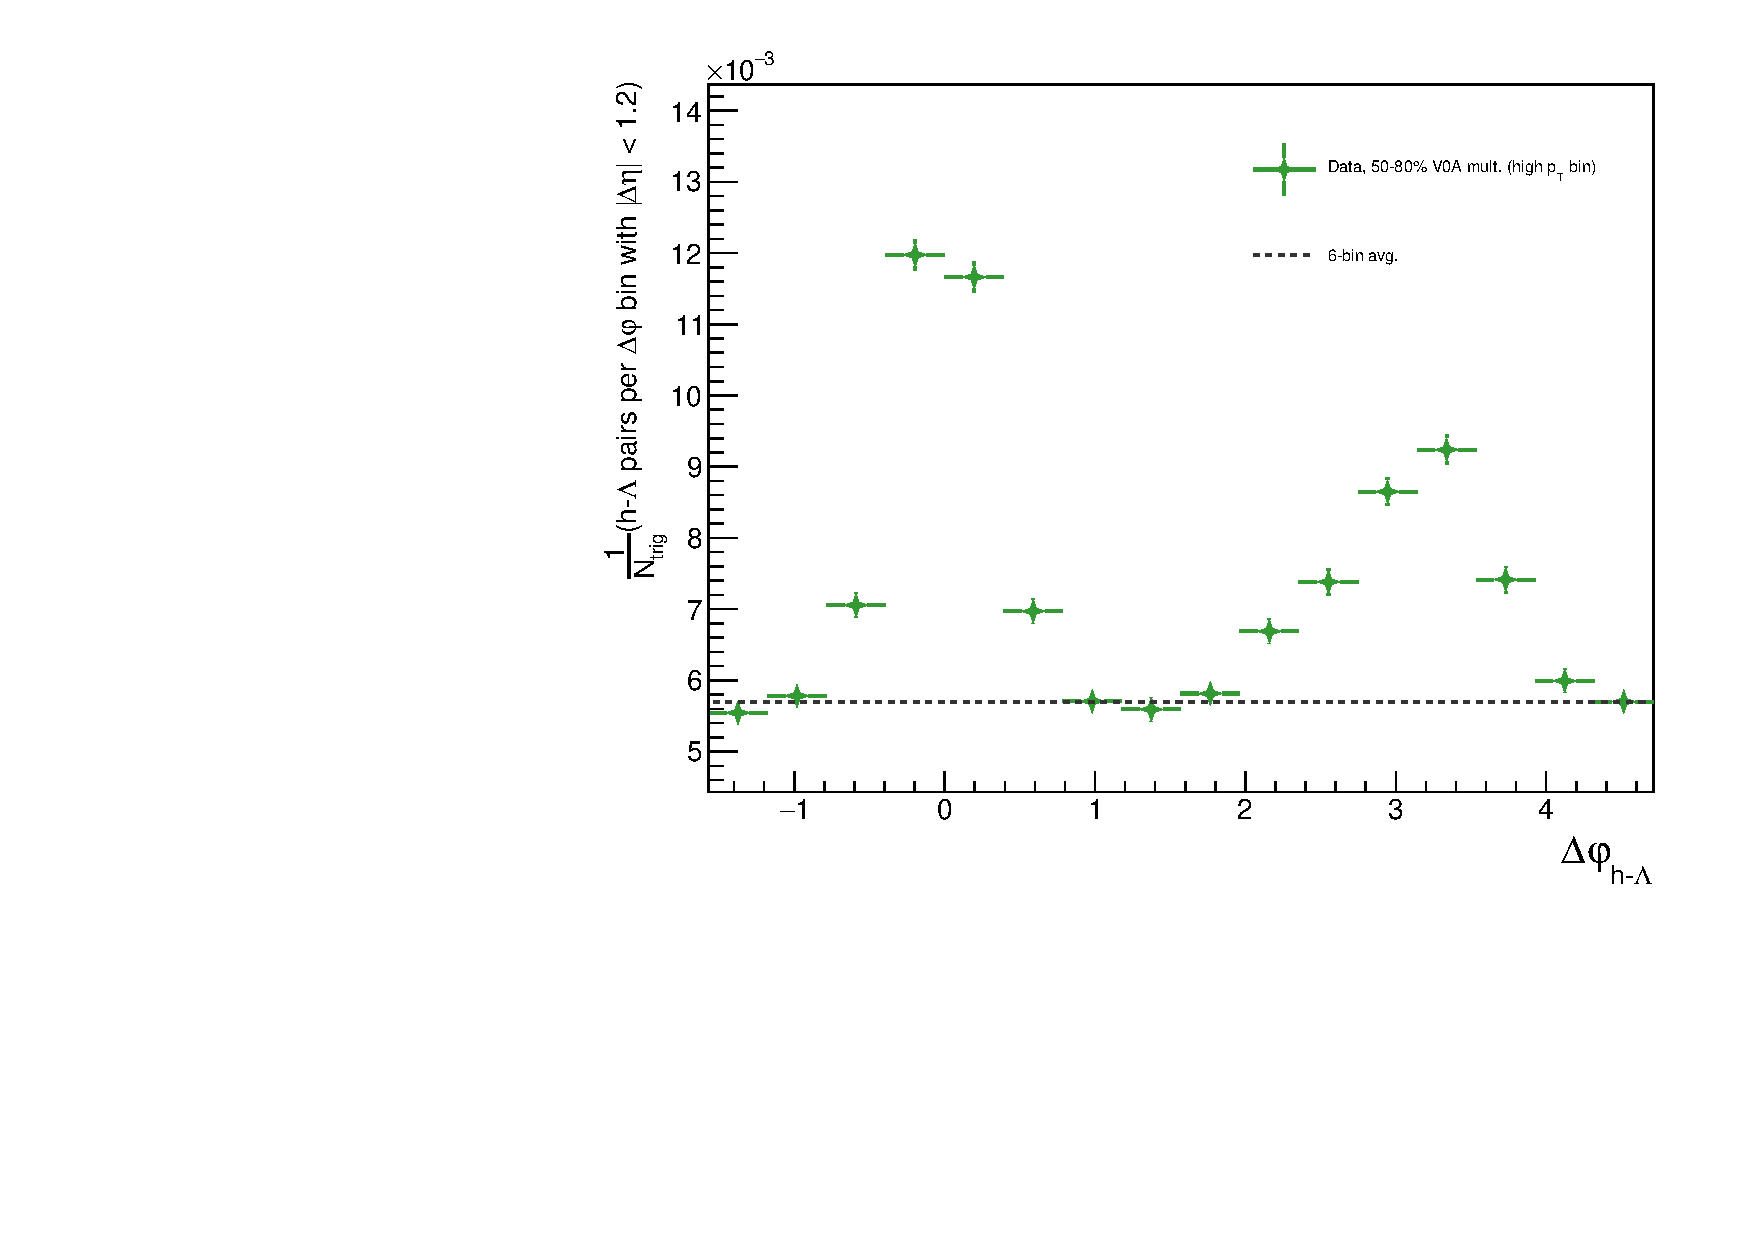
\includegraphics[width=\textwidth]{figures/analysis/h_lambda_dphi_avg6_50_80_highpt.pdf}
	\end{minipage}
	\caption{The final per-trigger h-$\Lambda$ $\Delta\varphi$ distributions for the 0-20\% (top), 20-50\% (middle), and 50-80\% (bottom) multiplicity bins for $1.5 < p_{\text{T}} < 2.5$ GeV/$c$ (left) and $2.5 < p_{\text{T}} < 4.0$ GeV/$c$ (right).}
	\label{fig:h_lambda_1d_final}
\end{figure}

\begin{figure}[ht]
	\centering
	\begin{minipage}{0.48\textwidth}
		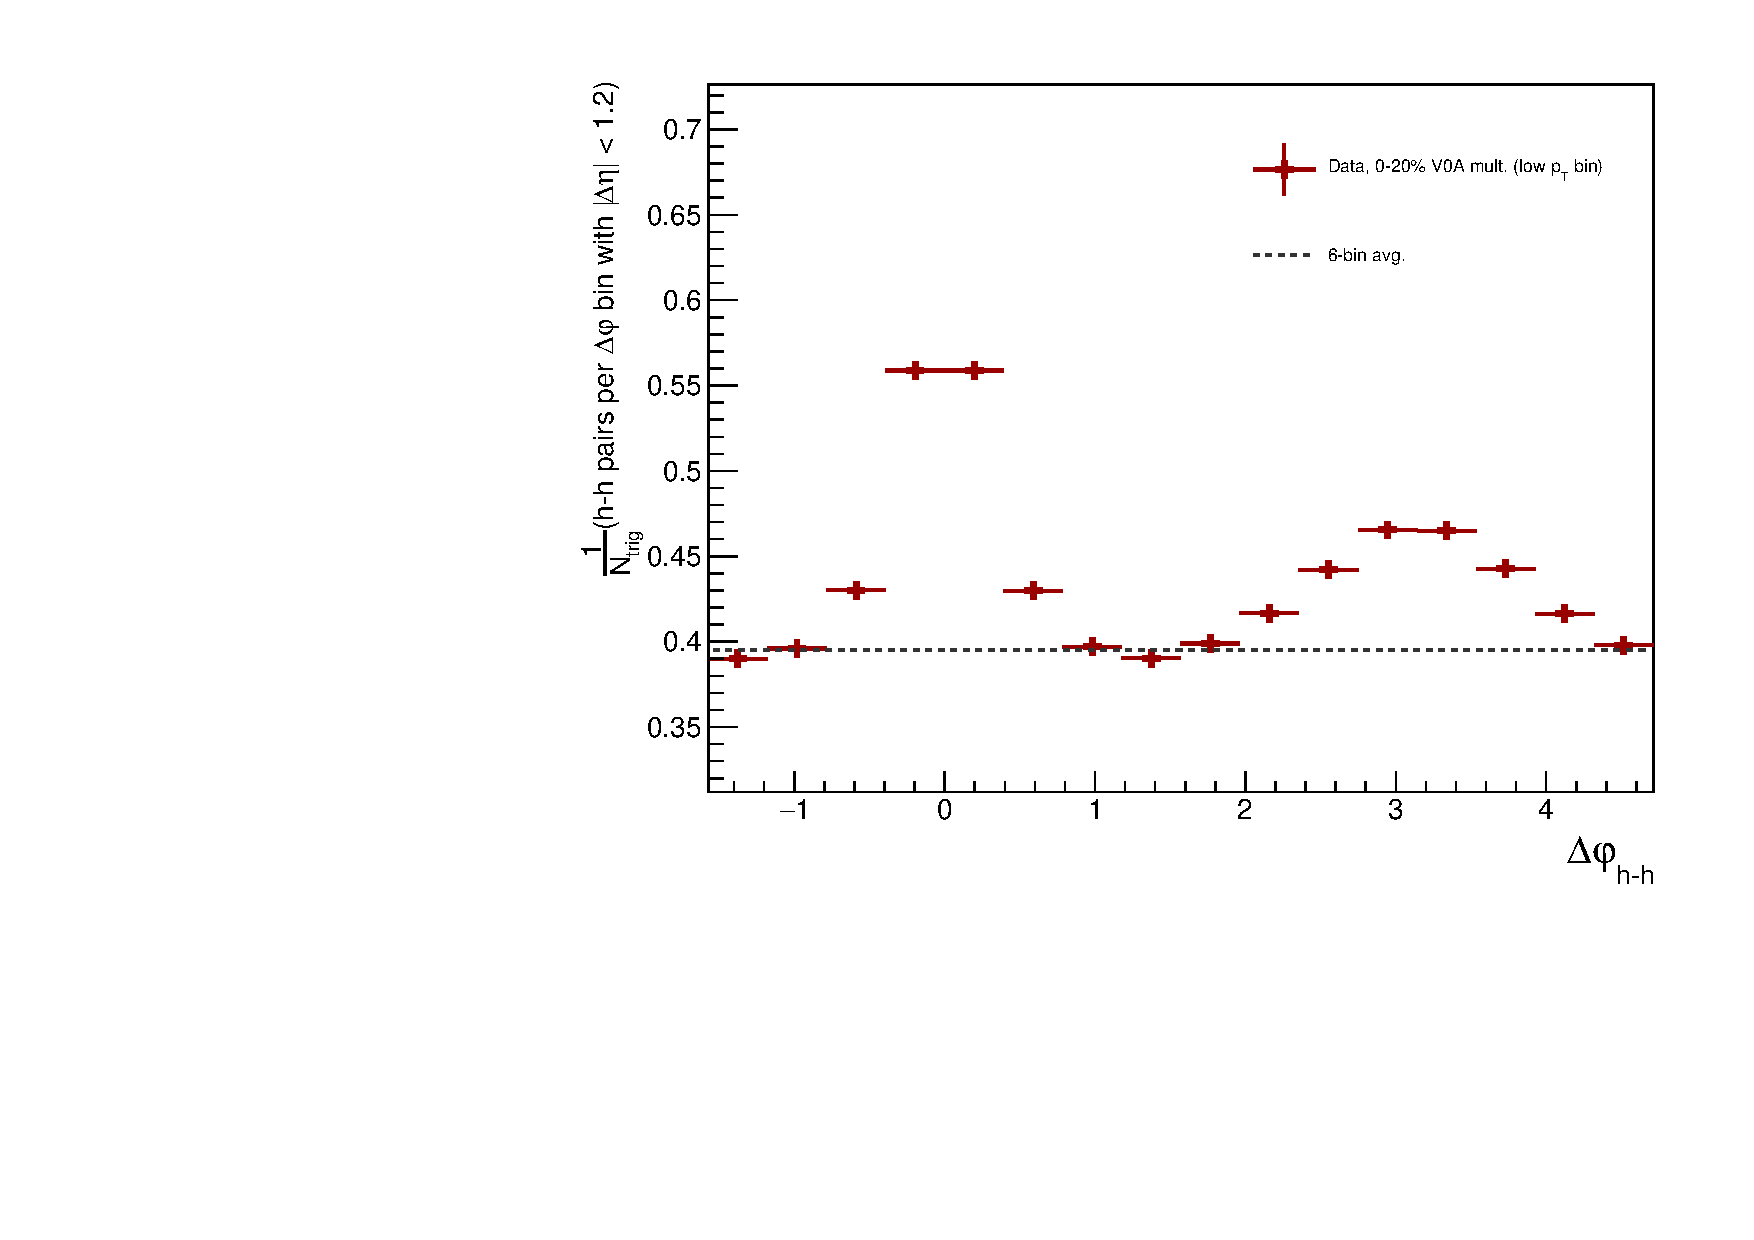
\includegraphics[width=\textwidth]{figures/analysis/h_h_dphi_avg6_0_20_lowpt.pdf}
	\end{minipage}
	\begin{minipage}{0.48\textwidth}
		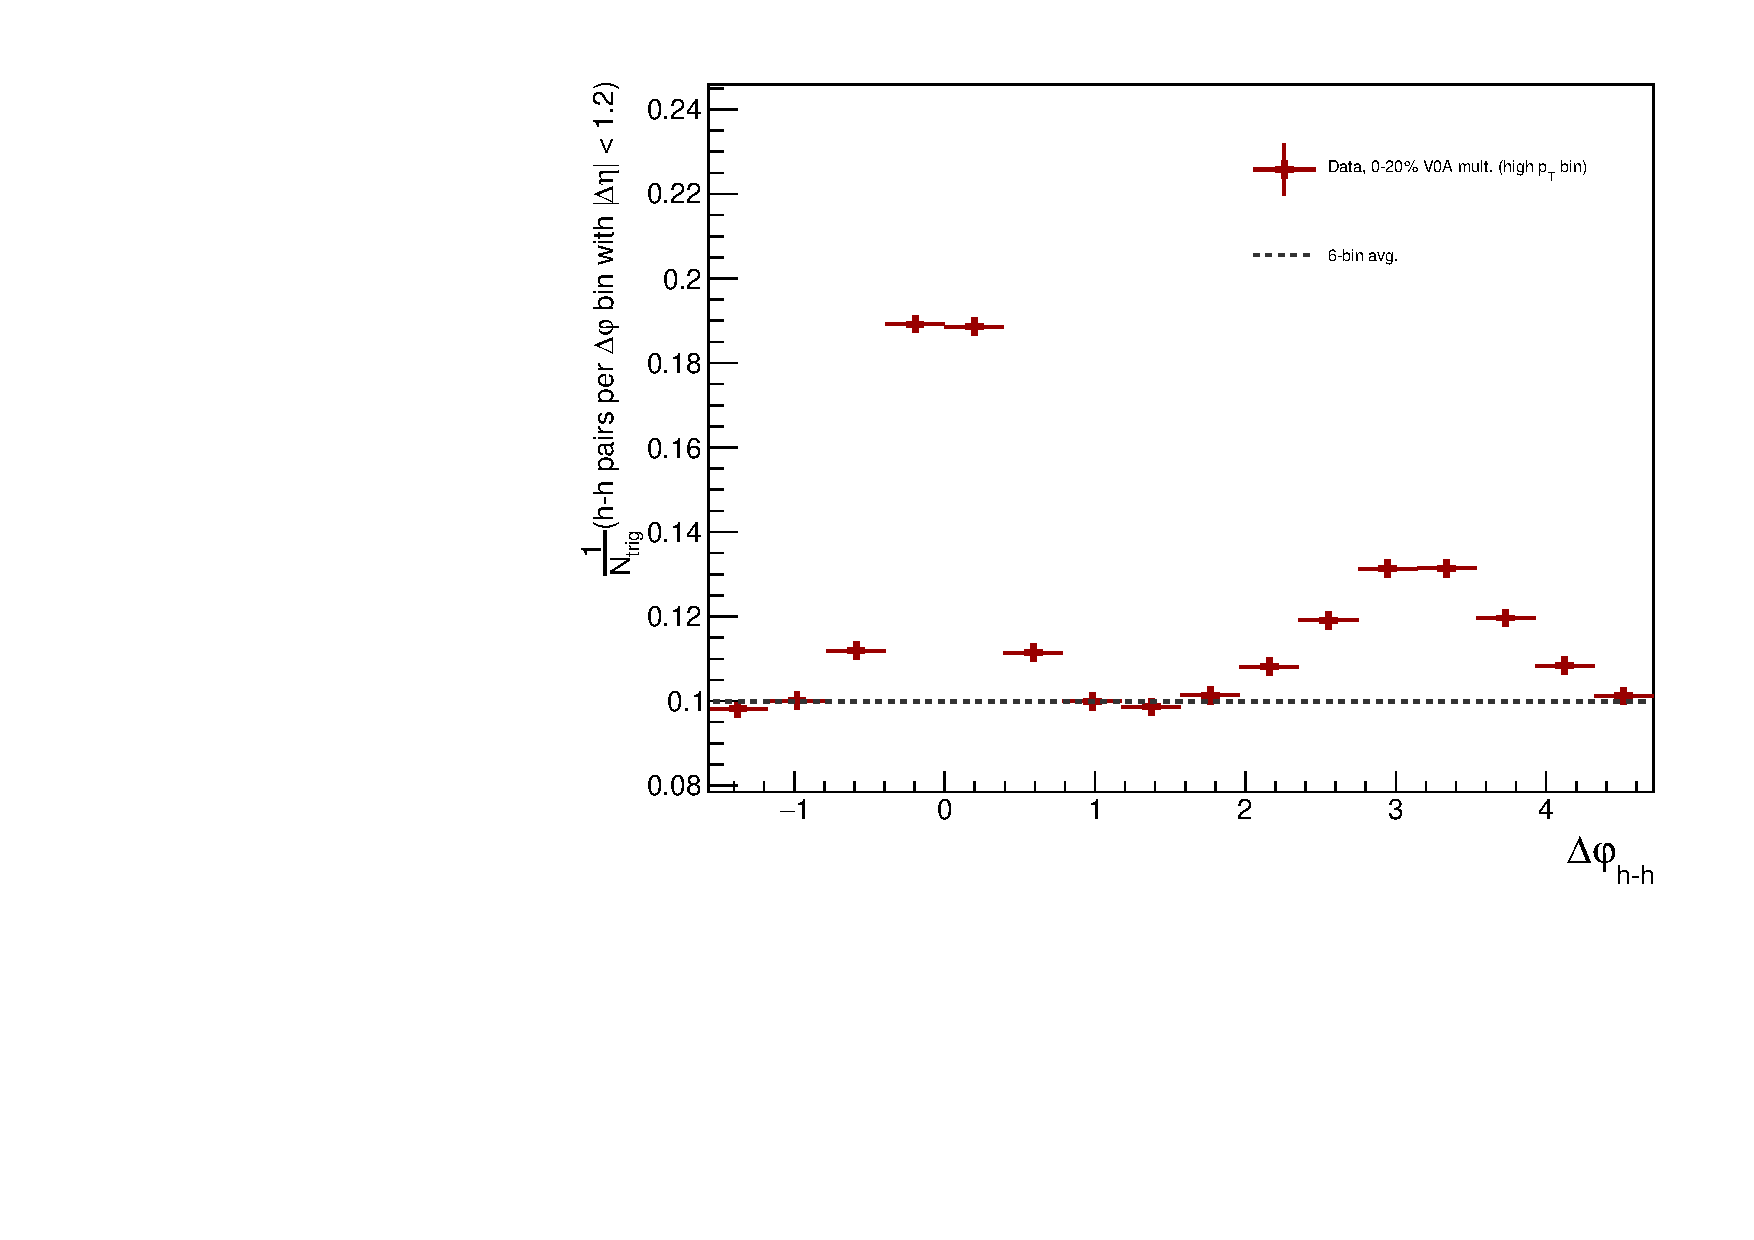
\includegraphics[width=\textwidth]{figures/analysis/h_h_dphi_avg6_0_20_highpt.pdf}
	\end{minipage}
	\begin{minipage}{0.48\textwidth}
		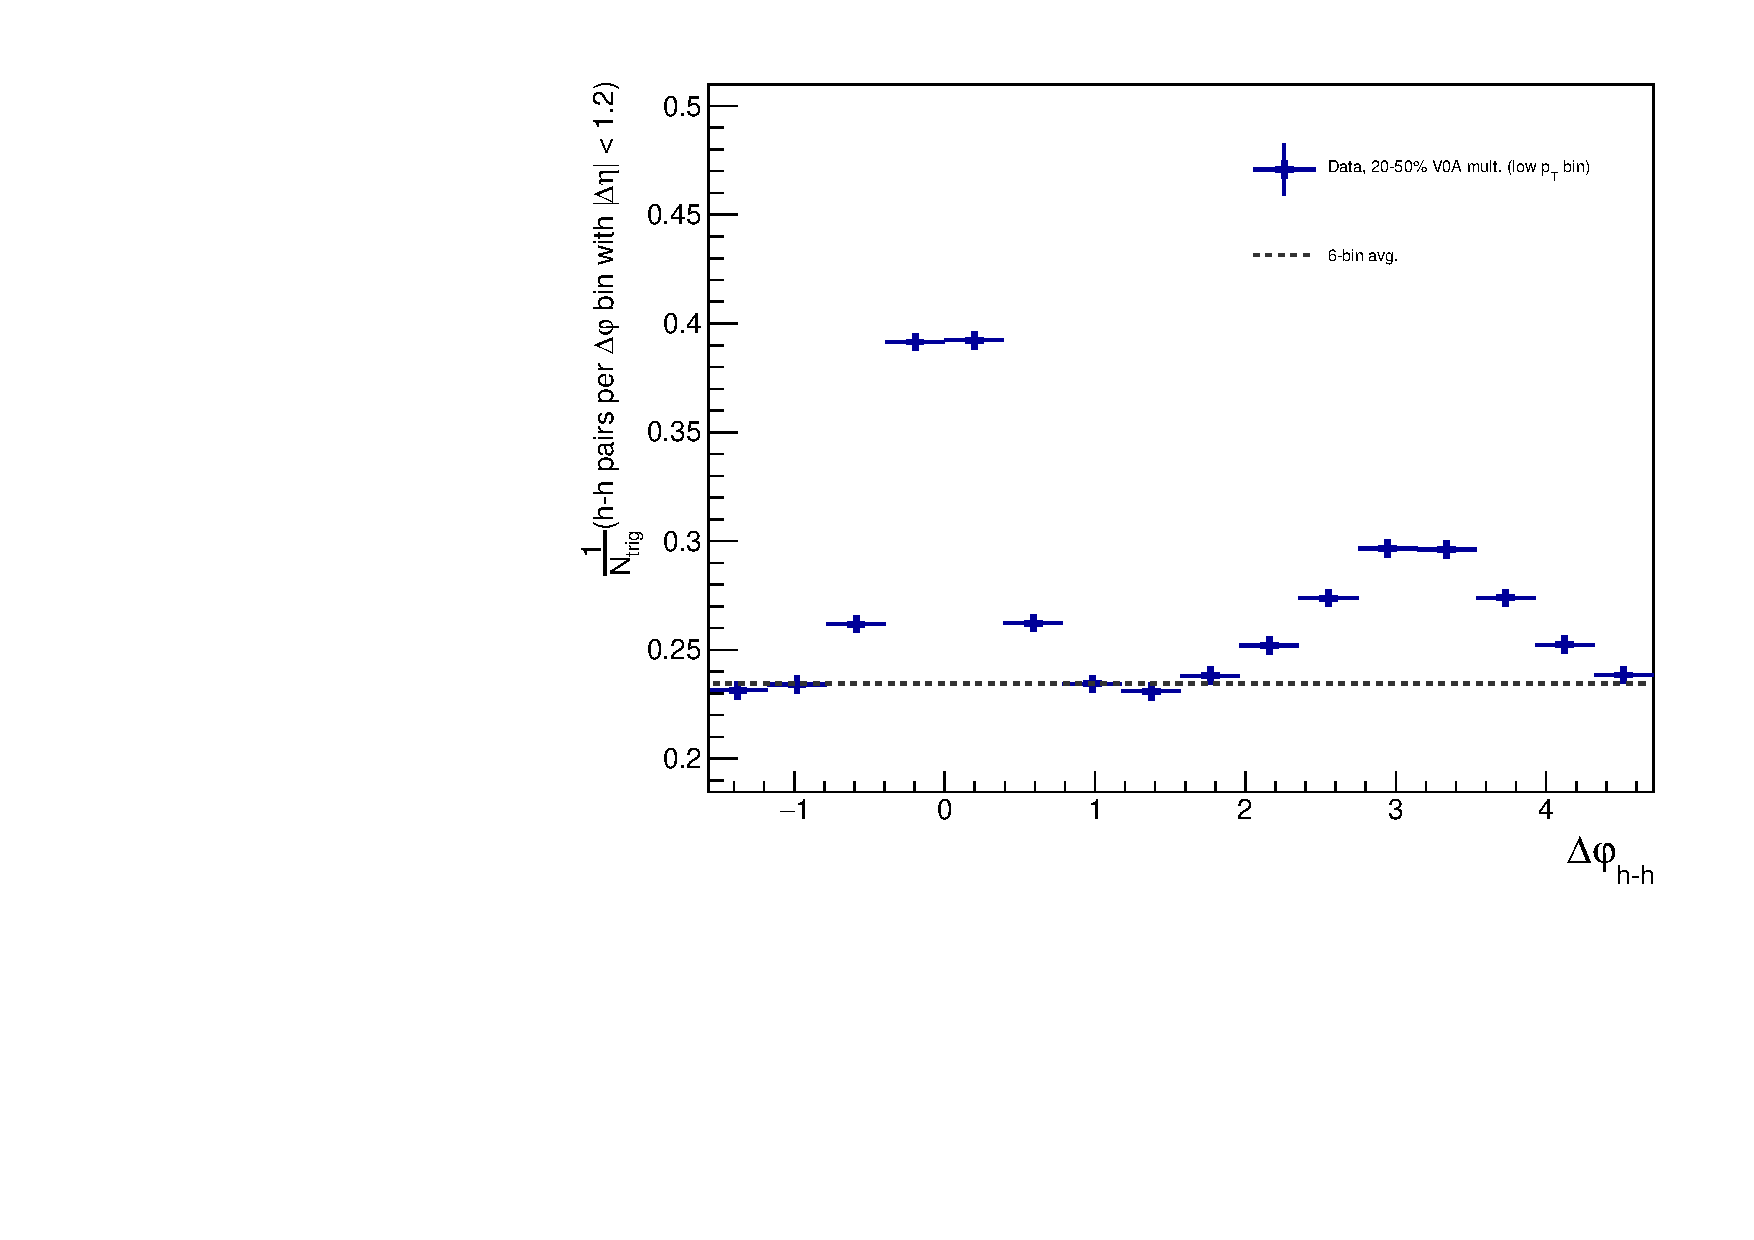
\includegraphics[width=\textwidth]{figures/analysis/h_h_dphi_avg6_20_50_lowpt.pdf}
	\end{minipage}
	\begin{minipage}{0.48\textwidth}
		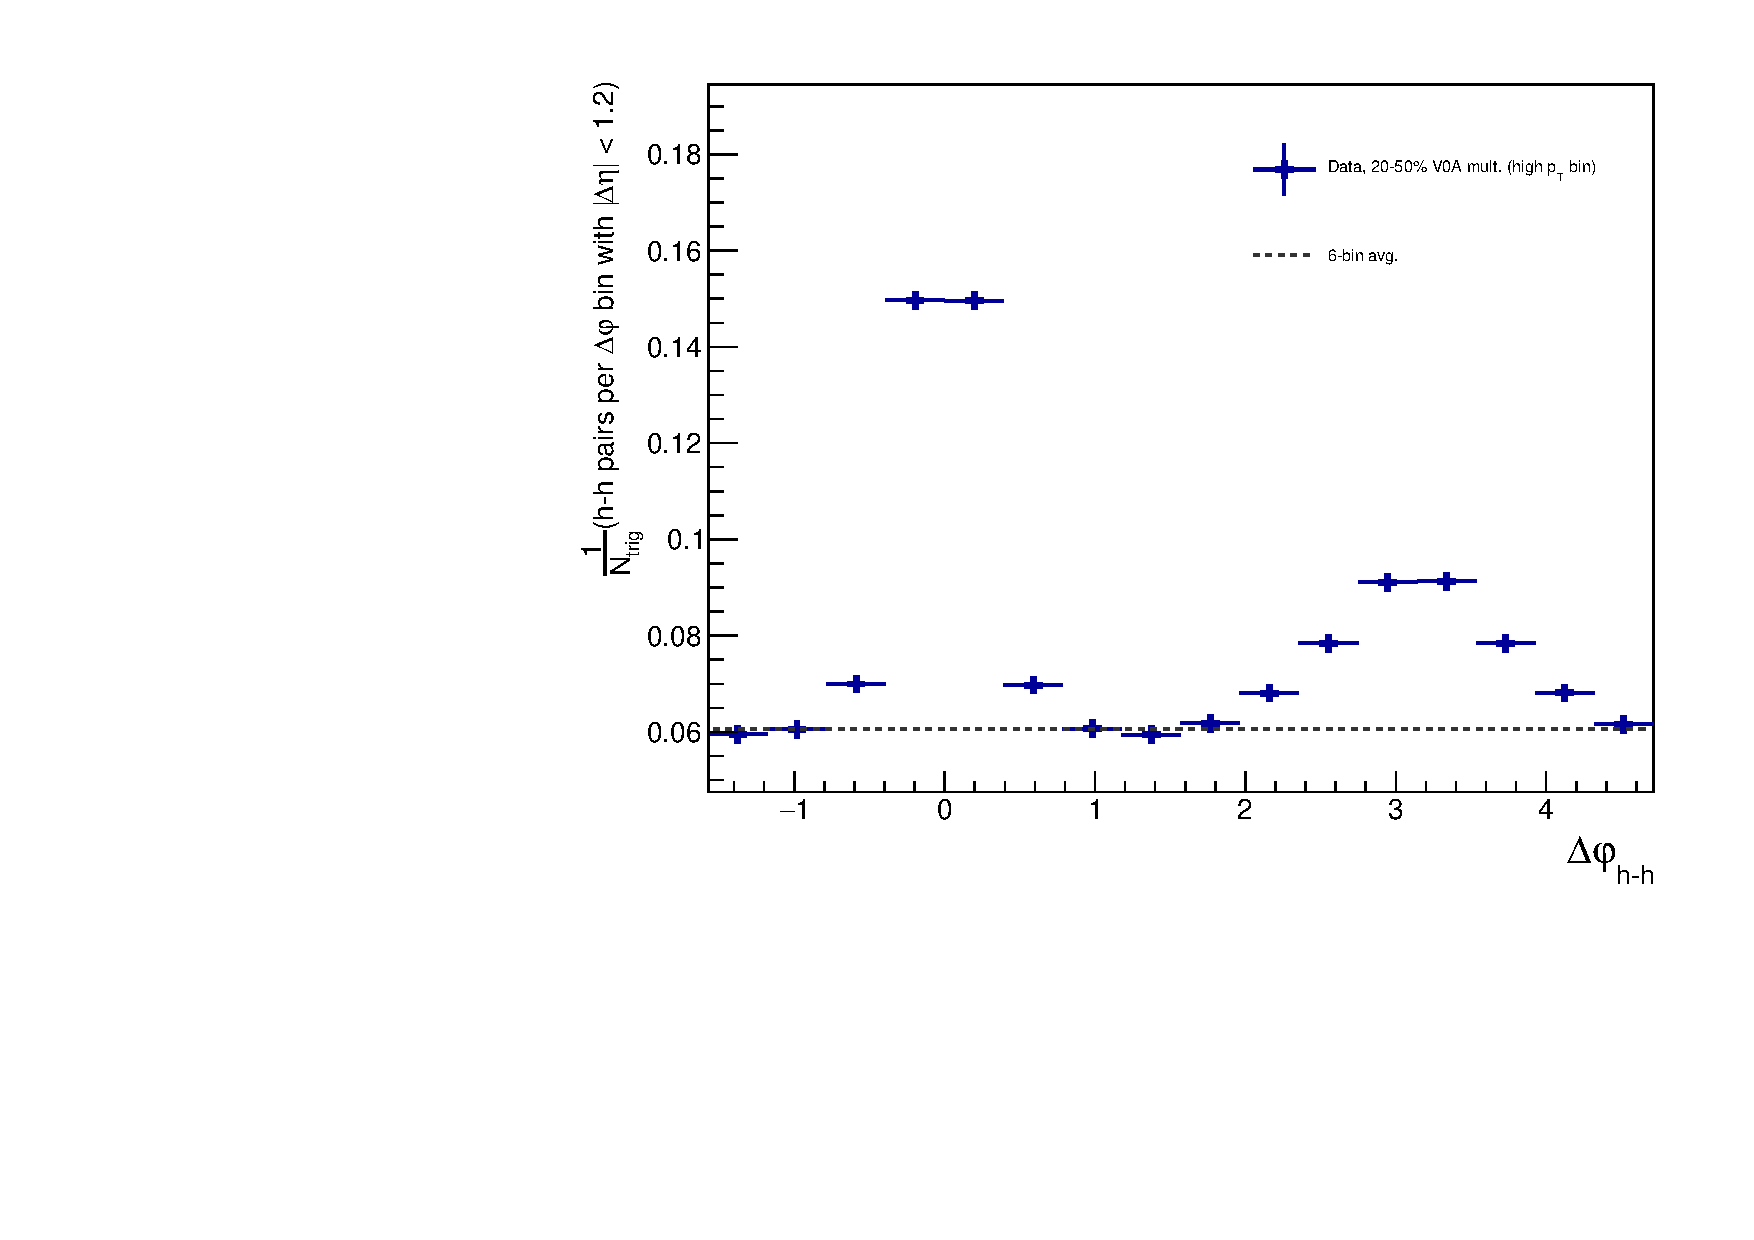
\includegraphics[width=\textwidth]{figures/analysis/h_h_dphi_avg6_20_50_highpt.pdf}
	\end{minipage}
	\begin{minipage}{0.48\textwidth}
		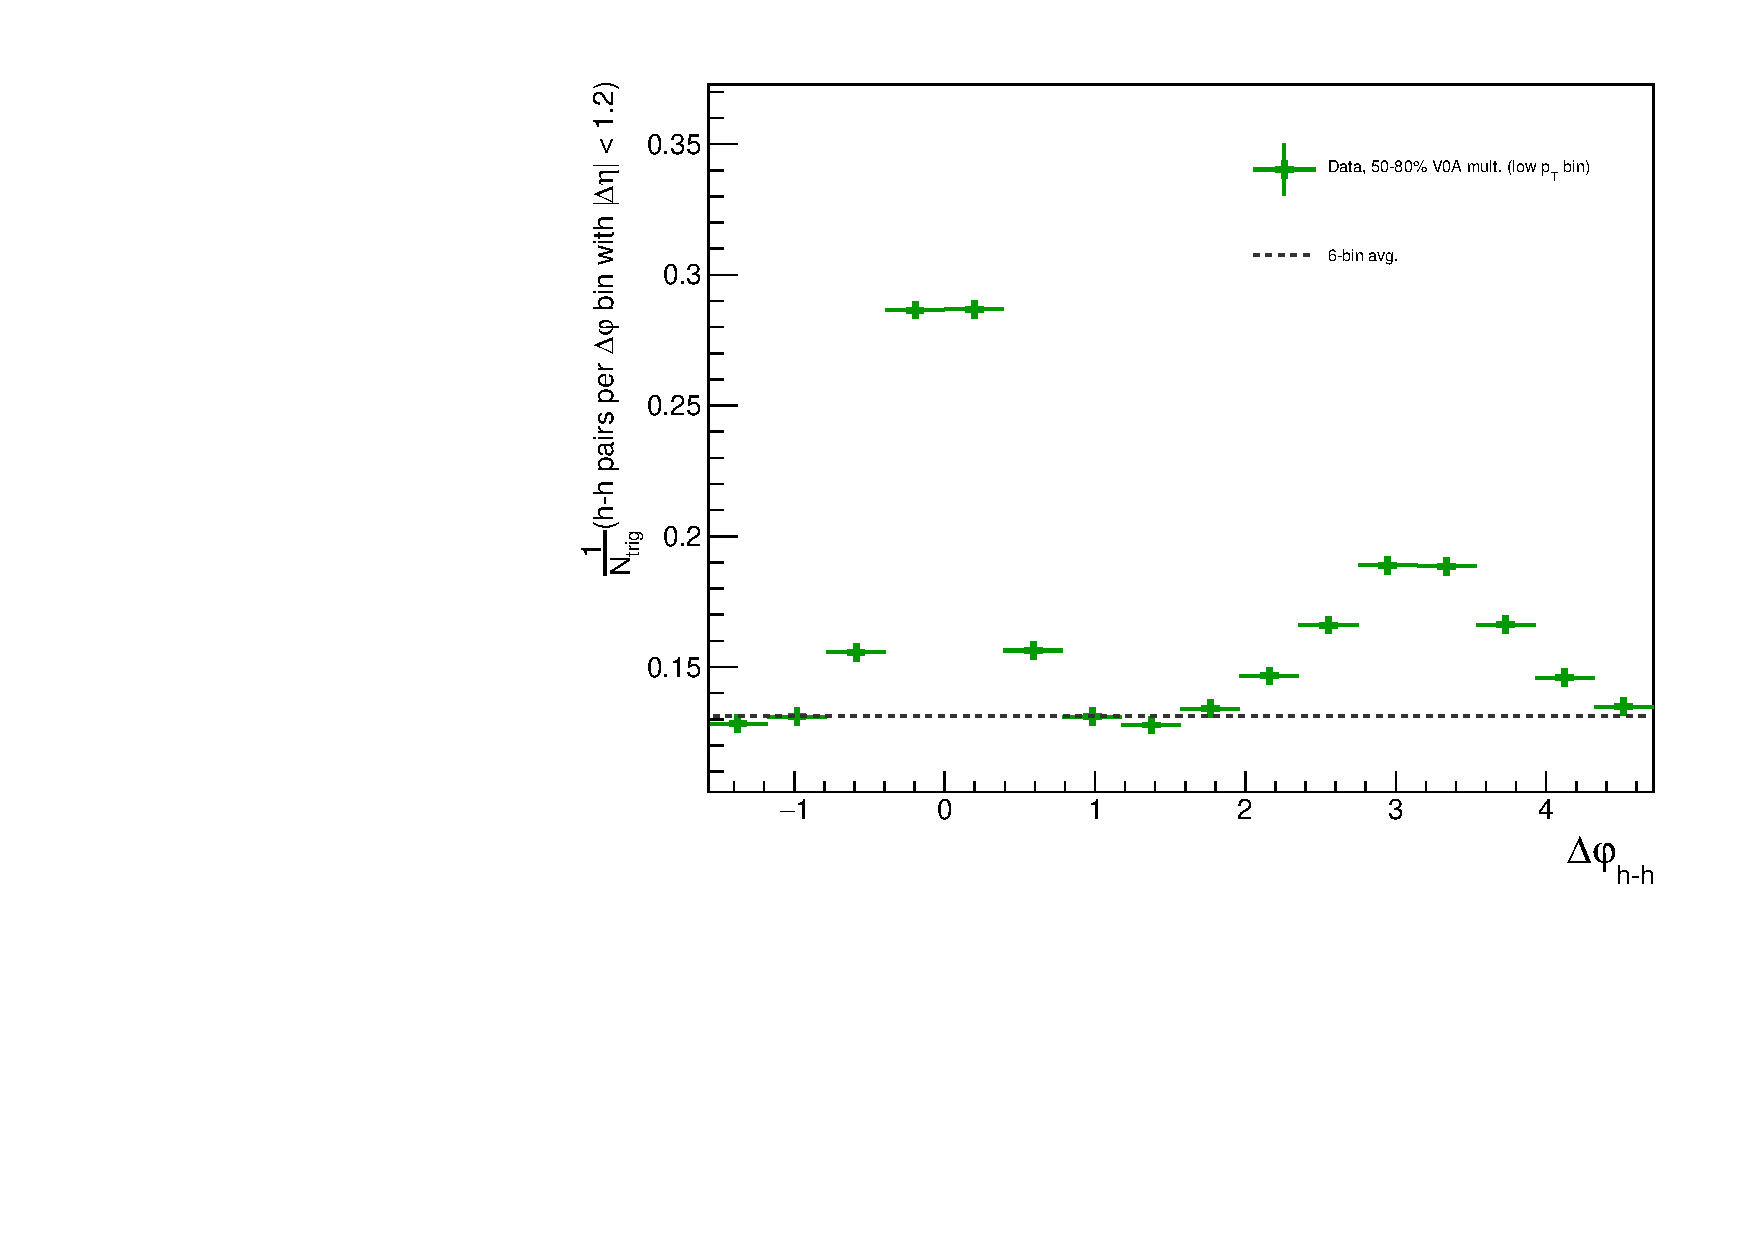
\includegraphics[width=\textwidth]{figures/analysis/h_h_dphi_avg6_50_80_lowpt.pdf}
	\end{minipage}
	\begin{minipage}{0.48\textwidth}
		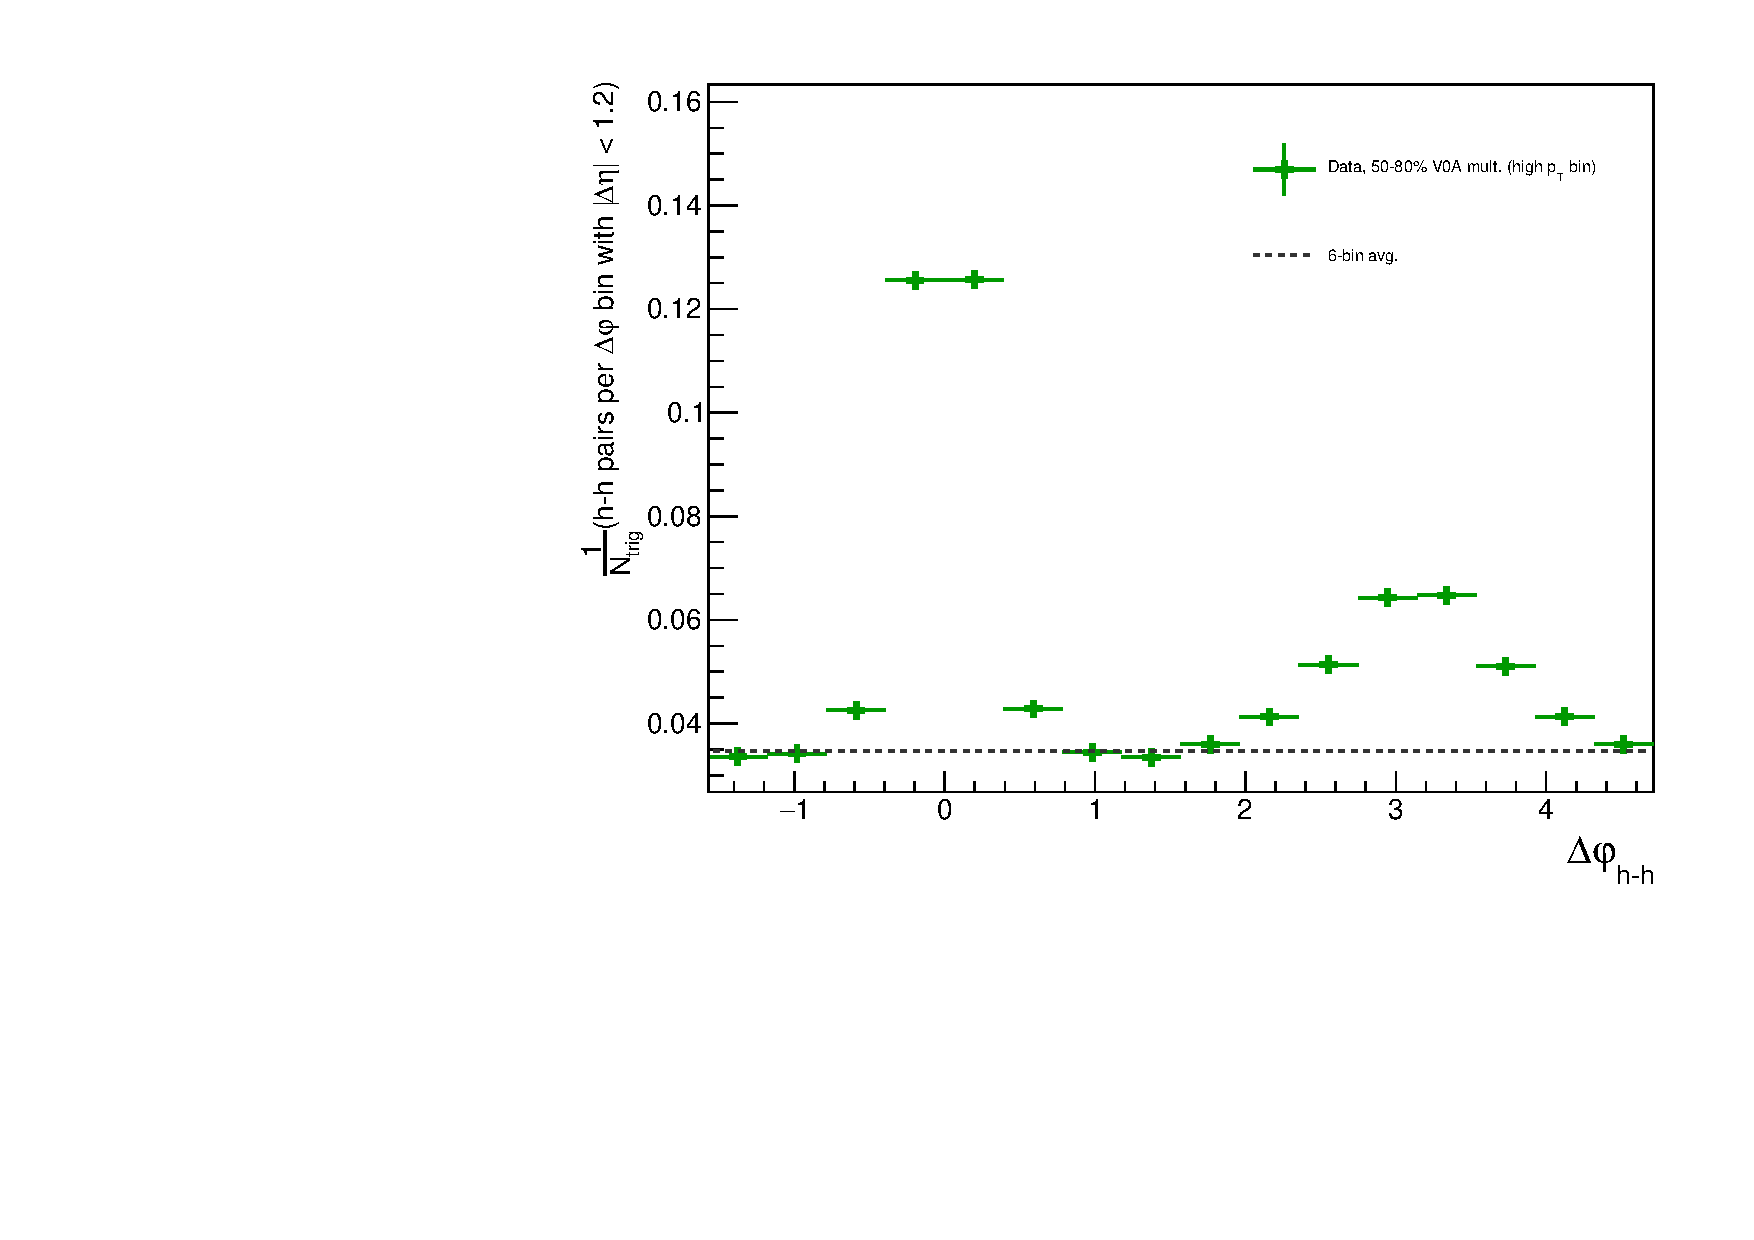
\includegraphics[width=\textwidth]{figures/analysis/h_h_dphi_avg6_50_80_highpt.pdf}
	\end{minipage}
	\caption{The final per-trigger h-h $\Delta\varphi$ distributions for the 0-20\% (top), 20-50\% (middle), and 50-80\% (bottom) multiplicity bins for $1.5 < p_{\text{T}} < 2.5$ GeV/$c$ (left) and $2.5 < p_{\text{T}} < 4.0$ GeV/$c$ (right).}
	\label{fig:h_h_1d_final}
\end{figure}

\begin{figure}[h!]
\centering
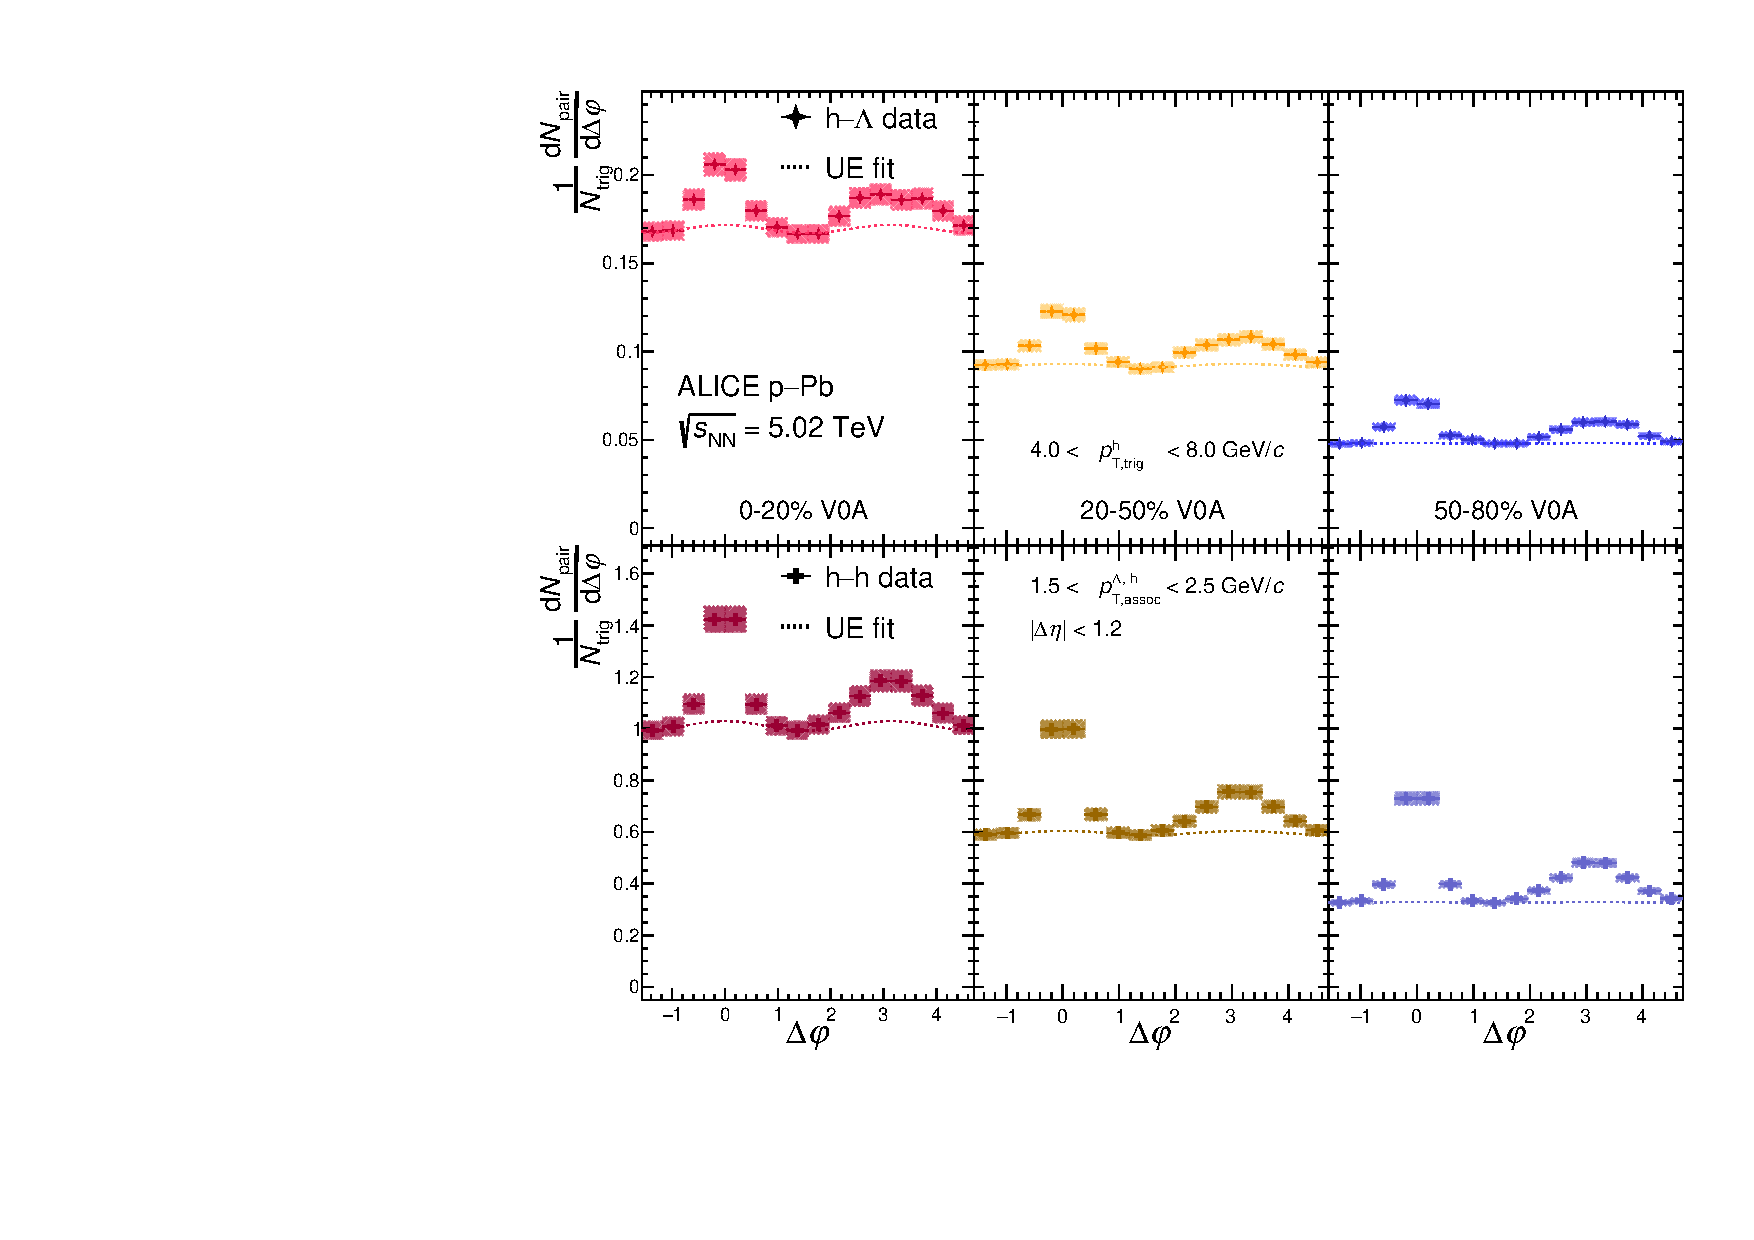
\includegraphics[width=0.83\textwidth]{figures/results/dphi_final_lowpt.pdf}
\caption{The h-$\Lambda$ (top) and h-h (bottom) $\Delta\varphi$ distributions for each multiplicity class with $1.5 < p_{\text{T,assoc}} < 2.5$ \GeVc, with statistical (systematic) uncertainties shown as vertical lines (shaded boxes). The multiplicity classes are plotted from most central (left) to least central (right). The UE estimate is shown as a dashed line, and is taken as the average of the distribution in the regions $[-\frac{\pi}{2}, -\frac{\pi}{4}) \cup [\frac{\pi}{4}, \frac{5\pi}{8}) \cup [\frac{11\pi}{8}, \frac{3\pi}{2})$.}
\label{fig:dphi_final_lowpt}
\end{figure}

\begin{figure}[h!]
\centering
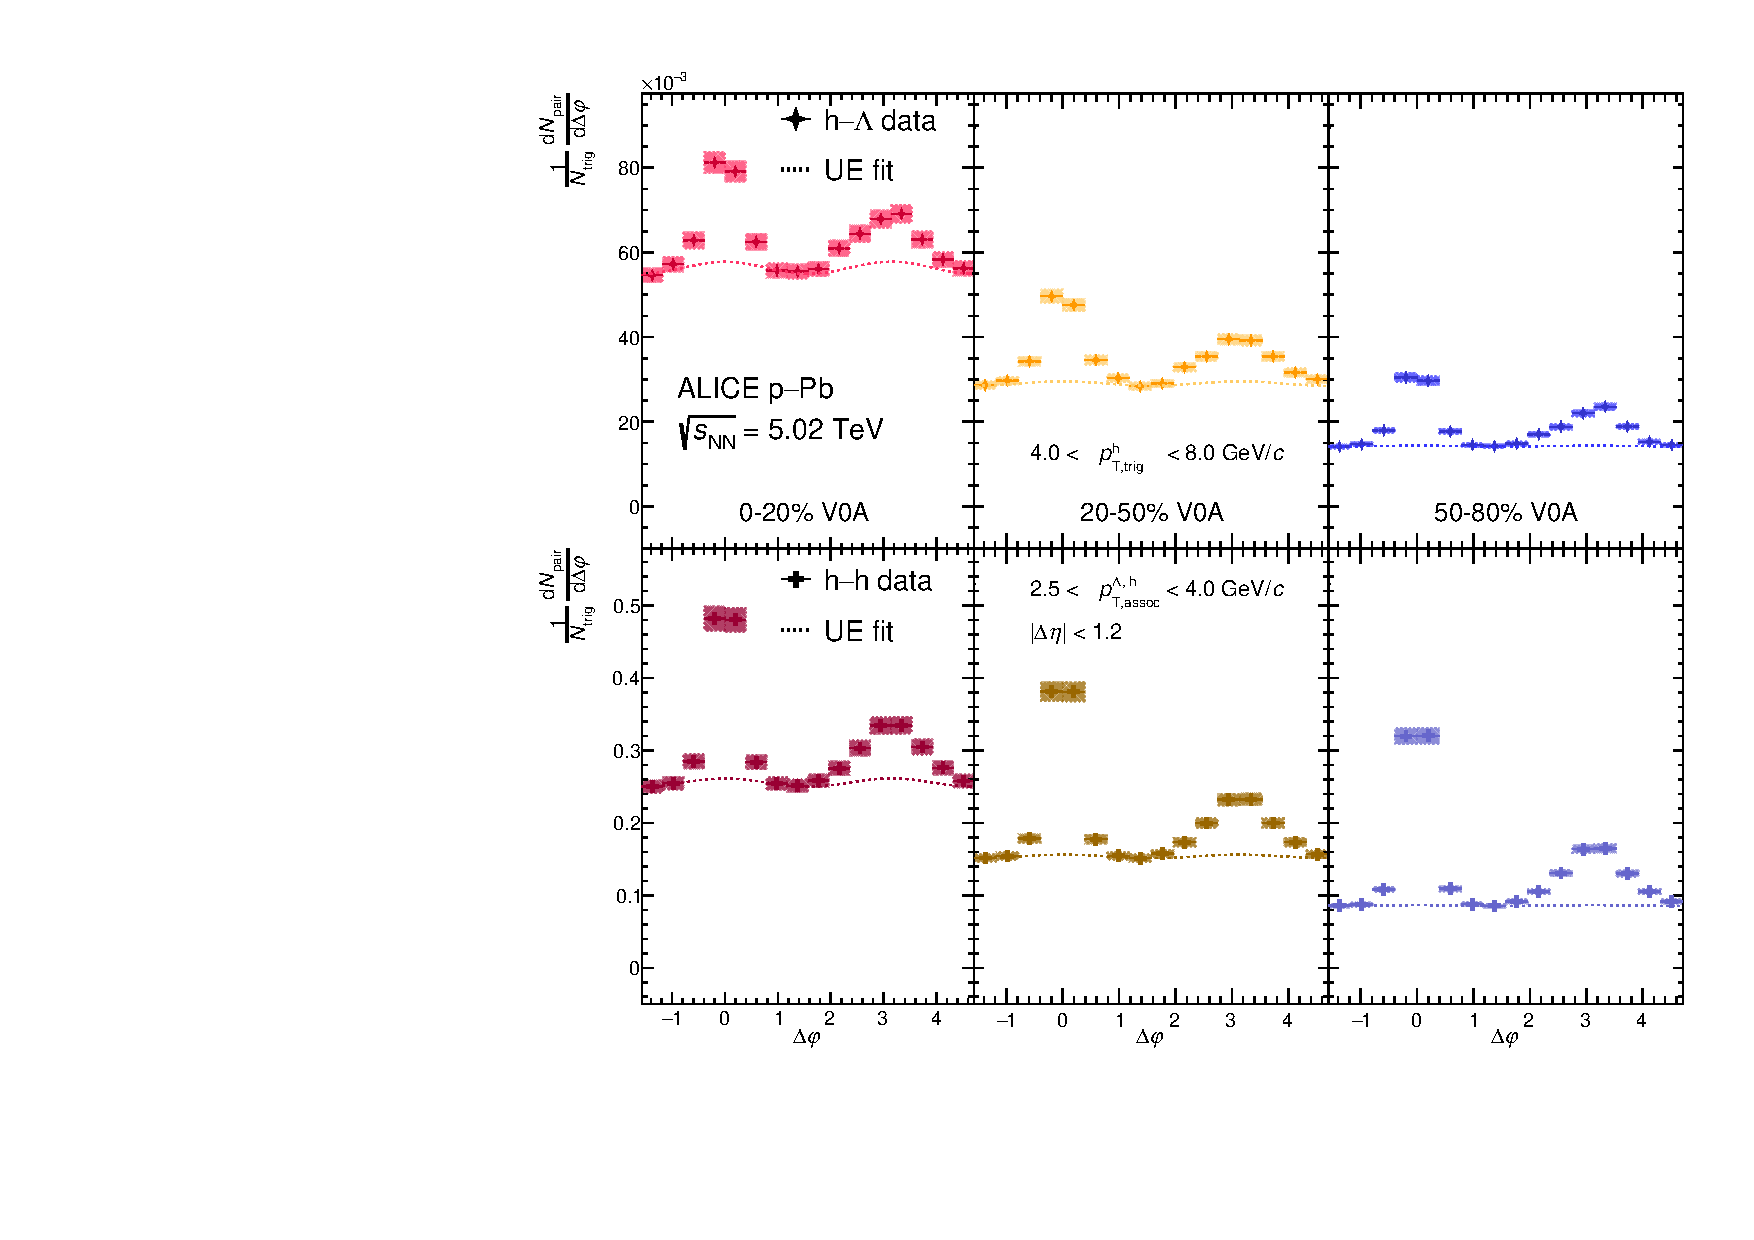
\includegraphics[width=0.83\textwidth]{figures/results/dphi_final_highpt.pdf}
\caption{The h-$\Lambda$ (top) and h-h (bottom) $\Delta\varphi$ distributions for each multiplicity class with $2.5 < p_{\text{T,assoc}} < 4.0$ \GeVc, with statistical (systematic) uncertainties shown as vertical lines (shaded boxes). The multiplicity classes are plotted from most central (left) to least central (right). The UE estimate is shown as a dashed line, and is taken as the average of the distribution in the regions $[-\frac{\pi}{2}, -\frac{\pi}{4}) \cup [\frac{\pi}{4}, \frac{5\pi}{8}) \cup [\frac{11\pi}{8}, \frac{3\pi}{2})$.}
\label{fig:dphi_final_highpt}
\end{figure}

\section{Per-trigger jet-like yields and jet widths}
\label{sec:jet_like_yield_width}

The per-trigger yields in the near- and away-side regions of the $\Delta\varphi$ distributions ($Y_{\text{near}}$, $Y_{\text{away}}$) are shown in each associated \pt range as a function of multiplicity percentile for both the h-$\Lambda$ and dihadron correlations in Figure \ref{fig:pairwise_yield}.

\begin{figure}[h!]
\centering
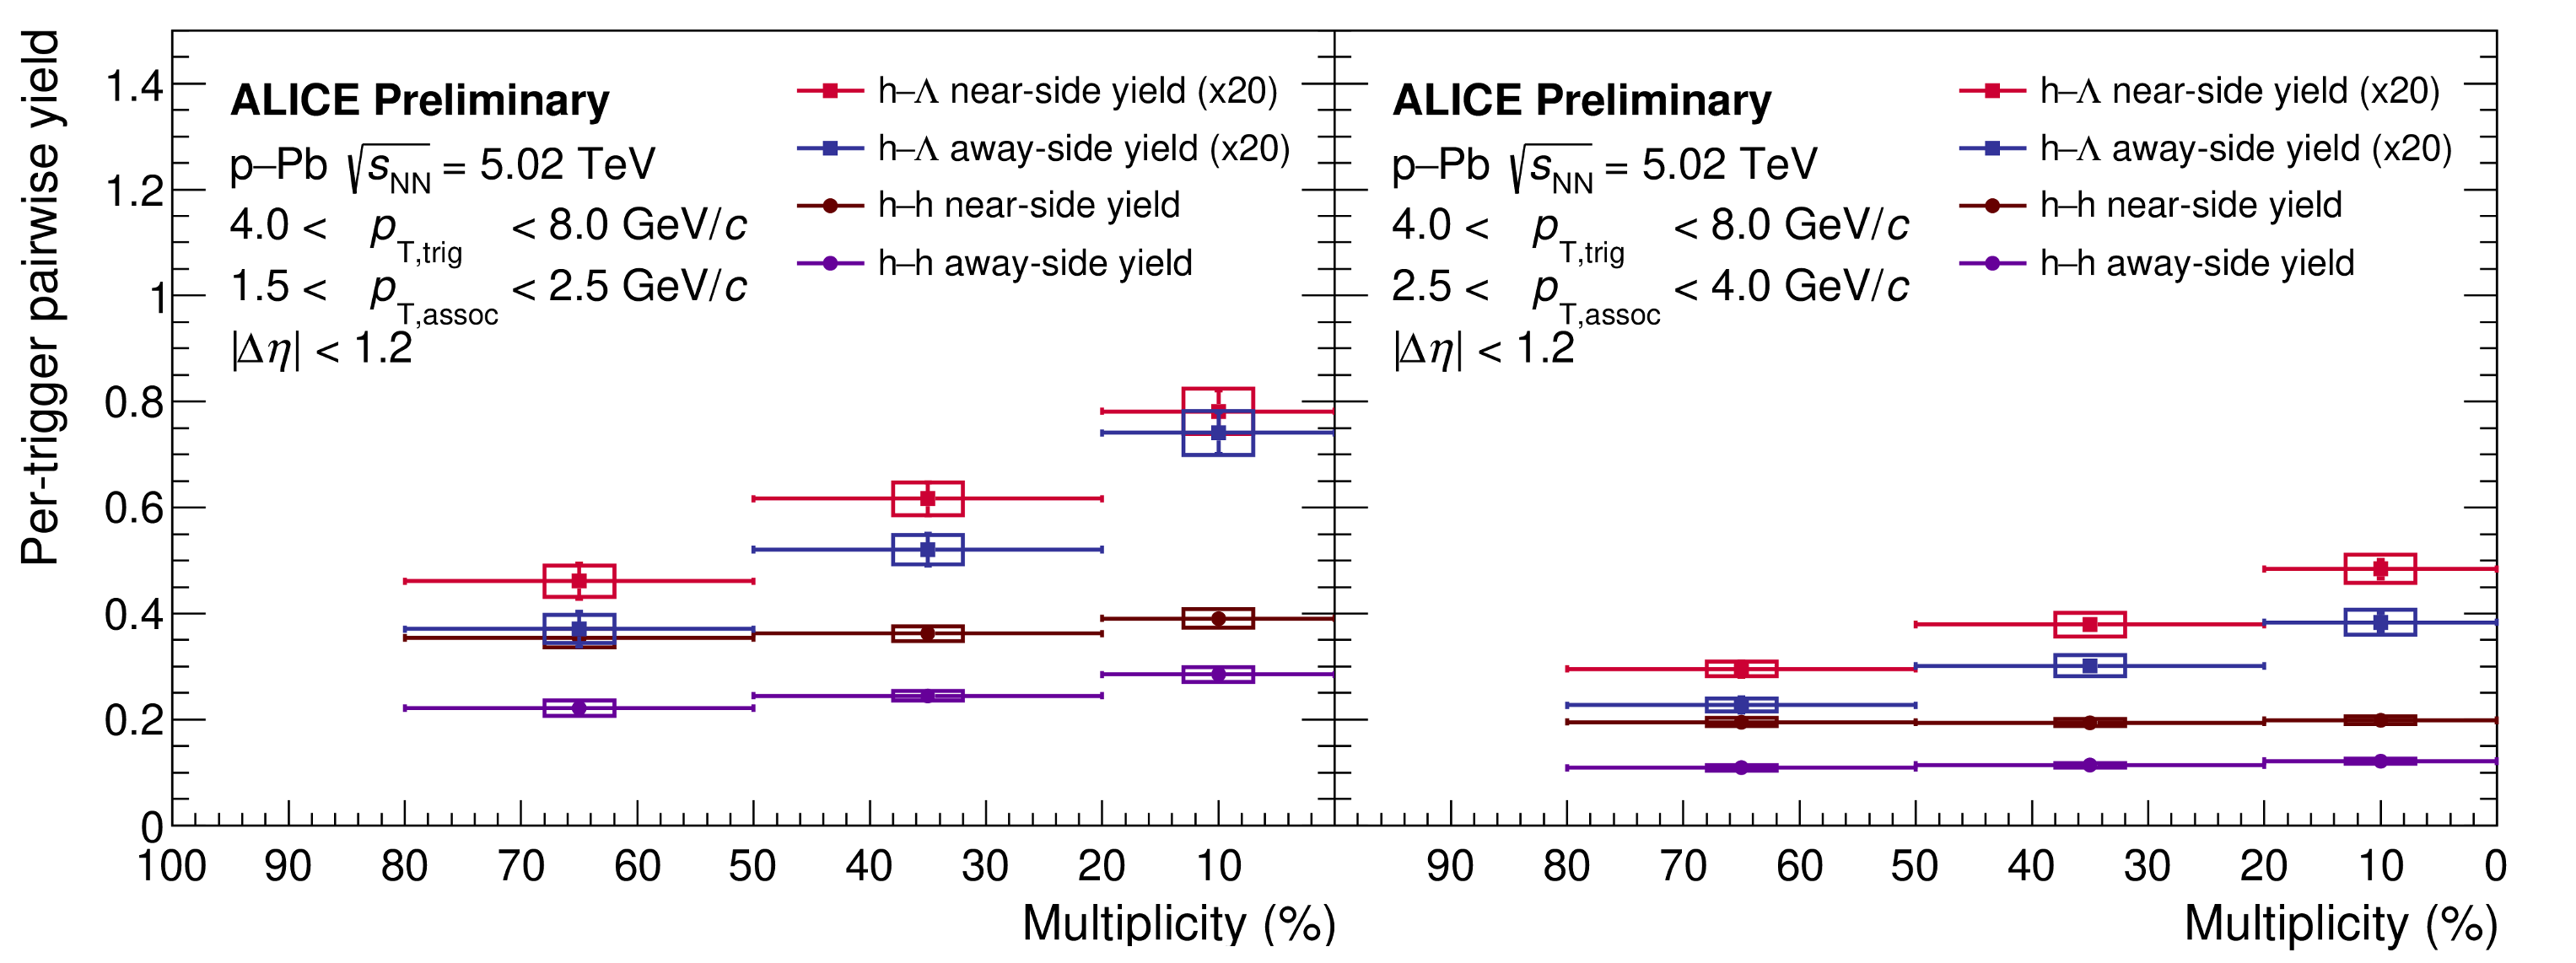
\includegraphics[width=\textwidth]{figures/results/pairwise_plot.png}
\caption{The per-trigger pair-wise yields $Y_{\text{near}}, Y_{\text{away}}$ as a function of multiplicity percentile for the h-$\Lambda$ (square markers) and h-h (circle markers) azimuthal correlations in the lower (left) and higher (right) associated \pt ranges. The statistical (systematic) uncertainties are shown as vertical lines (boxes).}
\label{fig:pairwise_yield}
\end{figure}

Across both associated \pt ranges, the h-$\Lambda$ yields see a substantial increase with respect to multiplicity for both the near- and away-side regions. This is in stark contrast to the dihadron yields, which see no significant increase as a function of multiplicity in both associated \pt ranges.  The increase can be quantified by calculating the percent change in the per-trigger yields from the lowest to highest multiplicity class, which is shown for each momentum range in Table \ref{tab:percent_increase}. The errors reported are calculated using both the systematic and statistical uncertainties summed in quadrature, and the significance is obtained by calculating the deviation in the percent change from zero in terms of the total error. The significance obtained from the h-$\Lambda$ yields across both regions and \pt ranges are all $>2\sigma$, indicating that the increase is statistically significant. However, the dihadron yields see no statistically significant increase in both regions across both momentum ranges. In the h-\lmb and h-h cases, the percent changes in the away-side yields are systematically higher than the changes in the near-side yields. These differences between the near- and away-side yields' behavior as a function of multiplicity hint at a possible modification of the away-side jet production due to interactions between the jet and the QGP medium.

\begin{table}
\centering
\caption{The percent change in the per-trigger yields from the lowest to highest multiplicity class in the lower and higher associated momentum ranges. The errors reported are obtained using the systematic and statistical uncertainties summed in quadrature. The reported significance is the number of standard deviations away from zero percent change.}
\begin{tabular}{l c c}
\hline
Region & Percent change for lower (higher) $p_{\text{T, assoc}}^{\text{h,}\Lambda}$ & Lower (higher) $p_{\text{T, assoc}}^{\text{h,}\Lambda}$ significance \\
\hline
h-$\Lambda$ near-side &  $47.9 \pm 16.8$ ($46.6 \pm 14.6$) & $ 2.9\sigma (3.2\sigma) $\\ 
h-$\Lambda$ away-side &  $71.0 \pm 22.5$ ($46.2 \pm 17.9$) & $3.2\sigma (2.6\sigma)$ \\
h-h near-side &  $ 0.4 \pm 7.5$ ($-3.9 \pm 4.3$) & $0.1\sigma (-0.9\sigma)$ \\
h-h away-side &  $11.7 \pm 12.3$ ($1.0 \pm 7.0$) & $0.9\sigma (0.1\sigma)$ \\
\hline
\end{tabular}
\label{tab:percent_increase}
\end{table}

To gain more insight to the underlying mechanisms responsible for strangeness production in jets, the widths of the near- and away-side peak regions are extracted from the h-$\Lambda$ and h-h $\Delta\varphi$ distributions using Equations \ref{eq:fullfit} and \ref{eq:width}. Plots of these widths as a function of multiplicity for both associated momentum ranges are shown in Figure \ref{fig:jet_widths}.

\begin{figure}[h!]
\centering
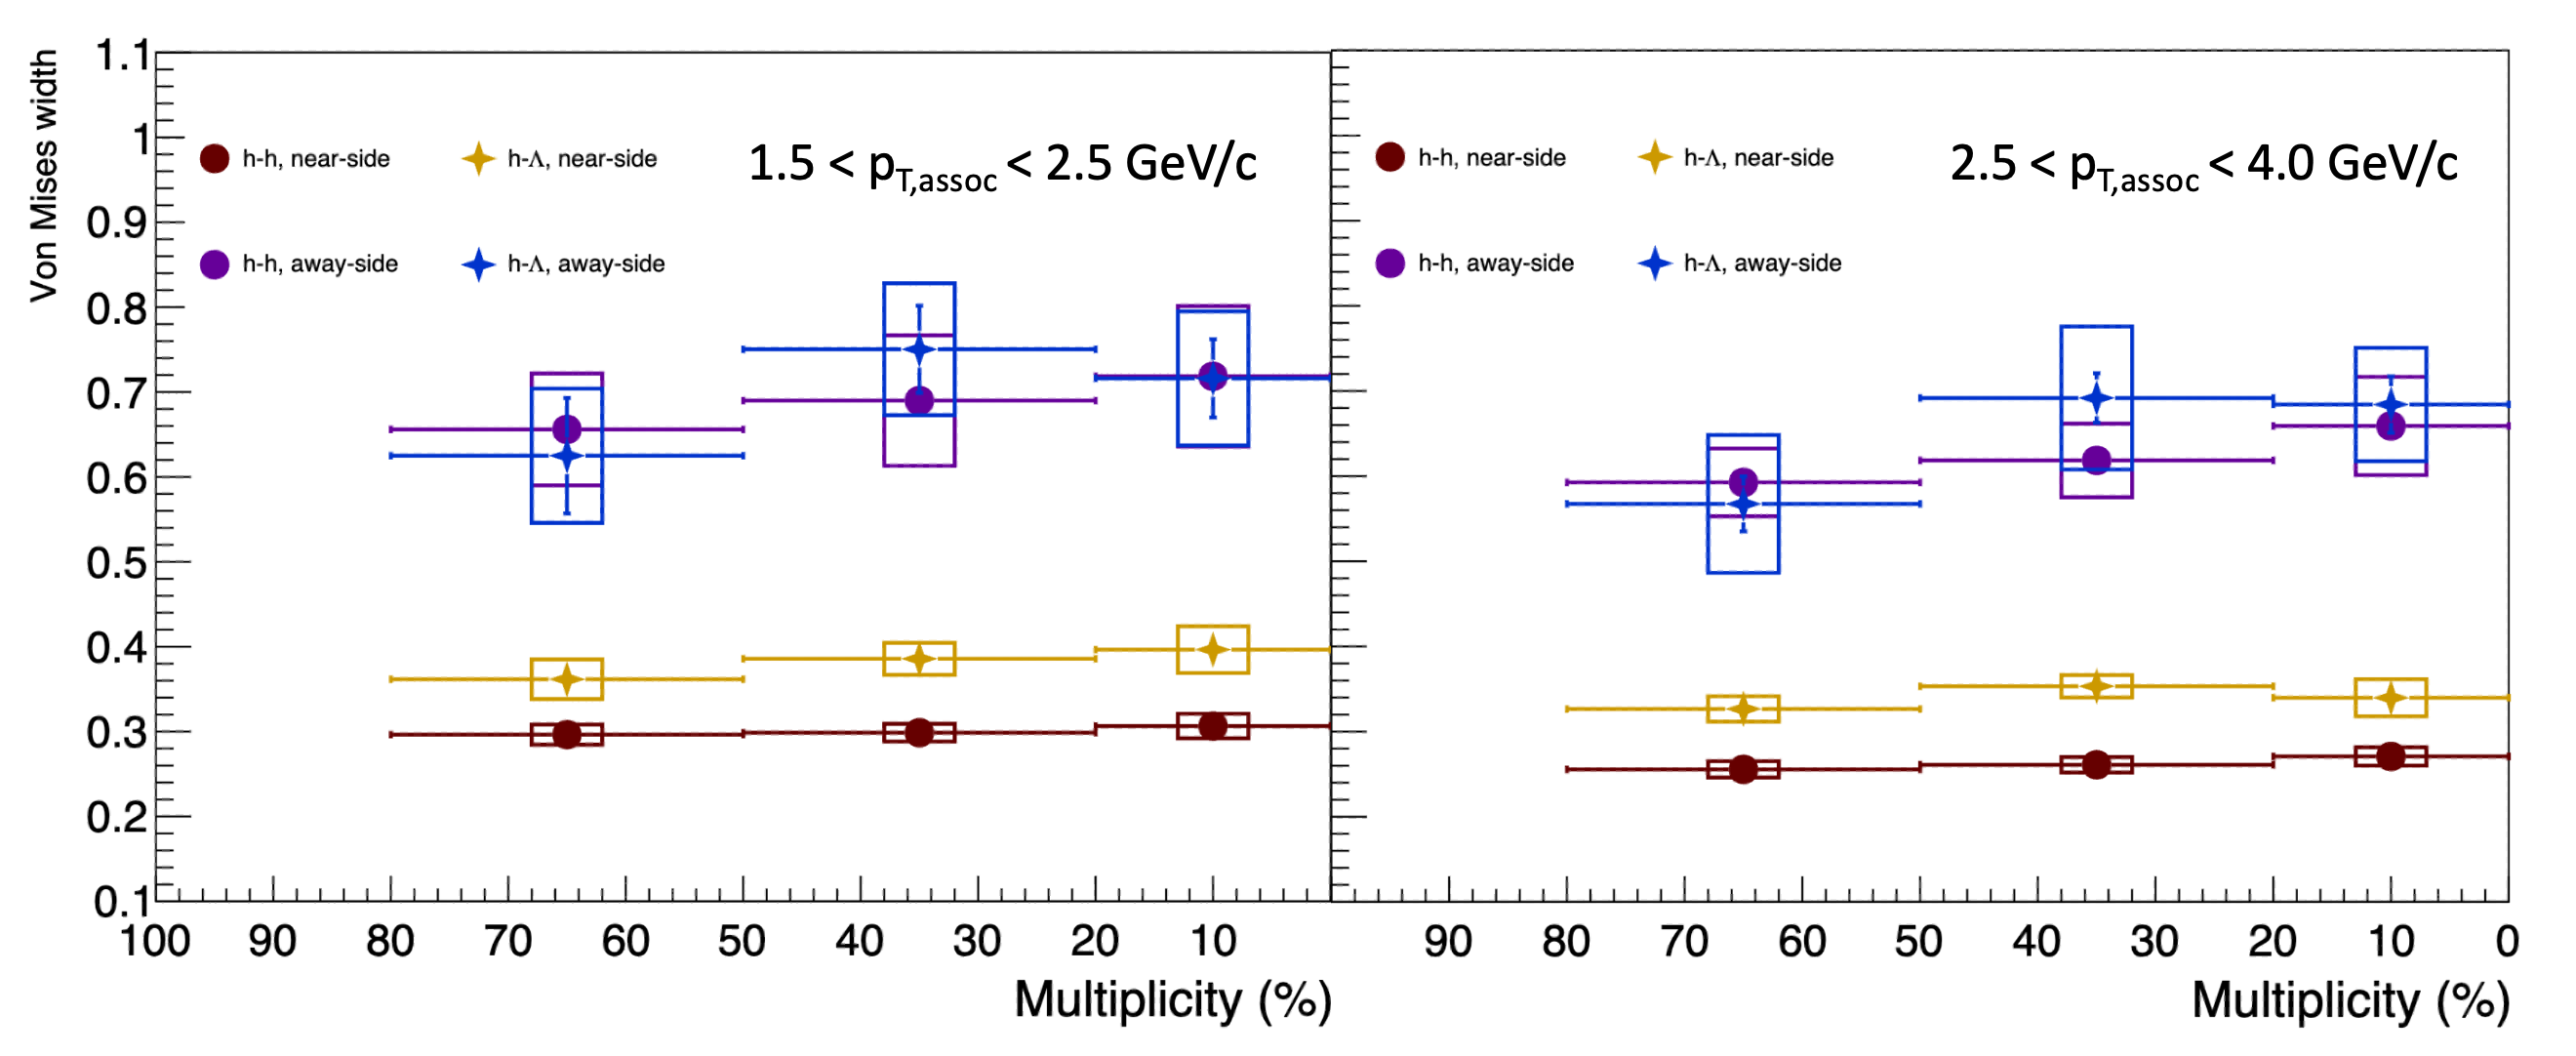
\includegraphics[width=\textwidth]{figures/results/widths_plot.png}
\caption{The h-$\Lambda$ and h-h near- and away-side peak widths shown as a function of multiplicity for both associated momentum ranges.  The statistical (systematic) uncertainties are shown as vertical lines (boxes).}
\label{fig:jet_widths}
\end{figure}

Expectedly, the near-side widths exhibit a significant decrease ($>$15\%) from the lower momentum range to the higher for both the h-$\Lambda$ and h-h cases, indicating that higher momentum associated particles are more collimated along the jet axis. An interesting result comes from comparing the h-$\Lambda$ and h-h away-side peak widths in data, which are found to be the same within systematic uncertainties across all multiplicity and momentum ranges, although the uncertainties are very large. This contrasts with the h-$\Lambda$ near-side widths, which are around 40\% ($2\sigma$) larger than the h-h widths across the entire multiplicity range for both momentum ranges. This indicates that the $\Lambda$ baryons are more readily produced in the periphery of the jet cone, which is unexpected. Due to conservation of fourmomentum, particles with higher mass tend to be produced closer to the jet axis. As these results indicate that $\Lambda$ baryons are being produced farther away from the jet axis than the less massive charged hadrons (pions, kaons and protons), this hints at a different underlying jet-fragmentation mechanism for $\Lambda$ baryons than for charged hadrons. The away-side widths also exhibit a hint of broadening with increasing multiplicity, though the systematic errors are too large to exclude flat behavior.

\subsection{Per-trigger yield ratios}

To better understand the differences between $\Lambda$ and charged hadron production both in and out-of jets, the per-trigger yield ratios $R_{i}^{\Lambda/h} \equiv Y_{i}^{h-\Lambda}$/$Y_{i}^{h-h}$ ($i$ = near-side, away-side, UE) are measured as a function of multiplicity in both associated momentum ranges. These ratios serve as a proxy for the $\Lambda/\pi$ ratio in each region, and are shown in Figure \ref{fig:lambda_hadron_ratio}. Straight line fits to the data are shown as dashed lines, with slopes and corresponding errors reported in Table \ref{tab:lambda_hadron_slopes}. To improve comparibility with previous results~\cite{ALICEpPbEnhancement,ALICEppEnhancement}, the multiplicity classes have been converted to charged particle multiplicity by computing $\langle$\dndeta$\rangle$ in each multiplicity class in events with a trigger hadron for all charged hadrons with $|\eta| < 0.5$ and $p_{\text{T}} > 0.15$ \GeVc. The values of $\langle$\dndeta$\rangle$ for each multiplicity class in non-triggered and triggered events can be seen in Table~\ref{tab:dndeta}.

\begin{figure}[h!]
\centering
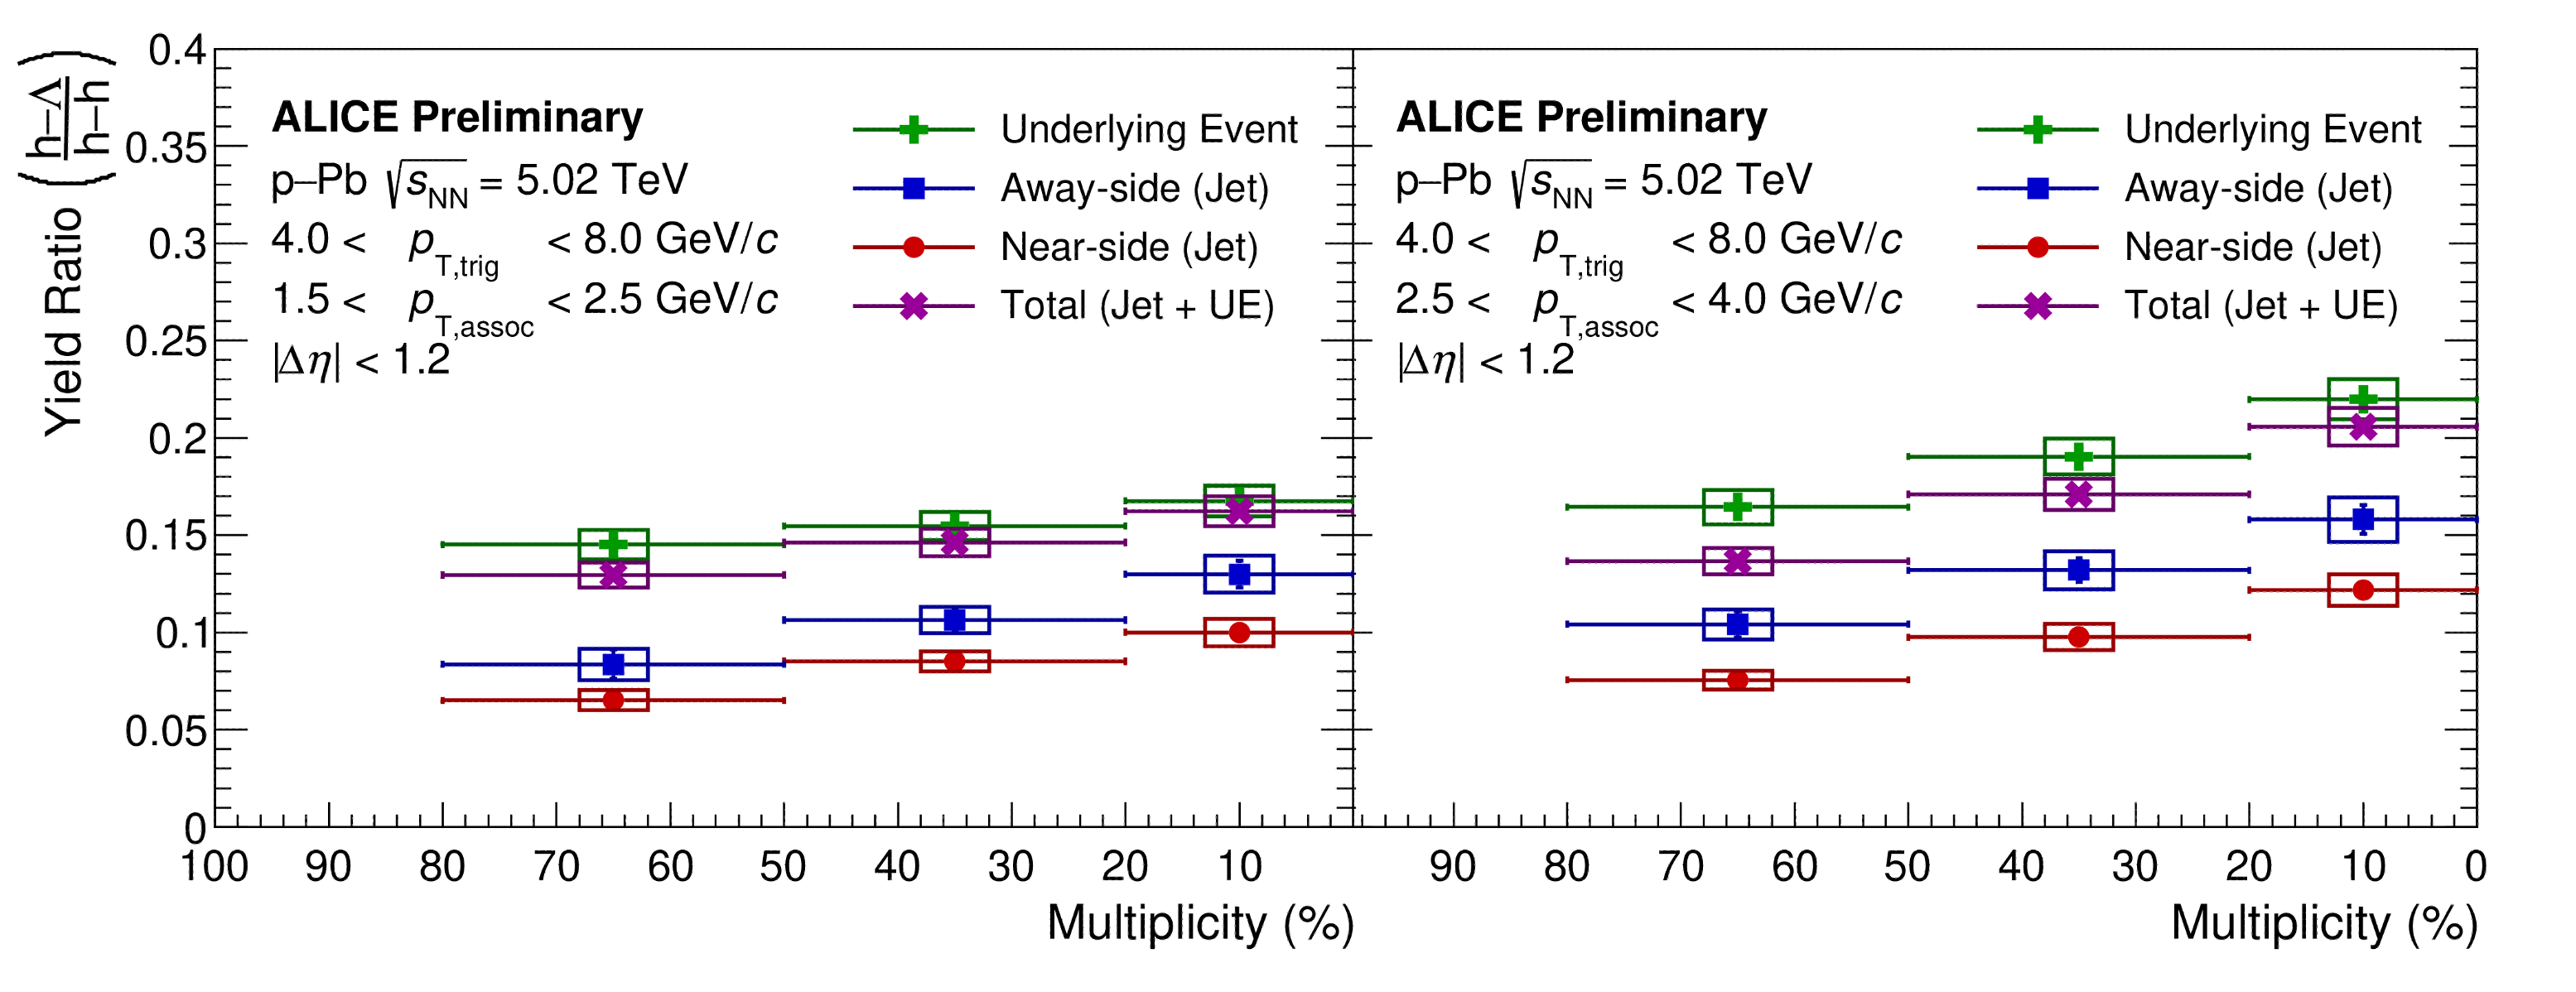
\includegraphics[width=\textwidth]{figures/results/ratio_plot.png}
\caption{The per-trigger yield ratios $R_{i}^{\Lambda/h} \equiv Y_{i}^{h-\Lambda}$/$Y_{i}^{h-h}$ ($i$ = near-side, away-side, UE) as a function of charged particle multiplicity for the lower (left) and higher (right) associated \pt ranges. The statistical (systematic) uncertainties are shown as vertical lines (boxes), and a first order polynomial fit to the data is shown as a dashed line.}
\label{fig:lambda_hadron_ratio}
\end{figure}

One surprising feature of these results is the clear separation between the ratios in each region across the entire multiplicity range in both momentum ranges, with the UE ratio being the largest, followed by the away-side ratio, and finally the near-side. This indicates that most of the relative $\Lambda$ production is occuring in the UE, which is consistent with the idea that $s$-quark production is maximal in the QGP medium. This is further supported by the fact that the away-side ratio is larger than the near-side, as $\Lambda$ production on the away-side is likely due to both the fragementation of the away-side jet coupled with the possible production of strange quarks due to jet-medium interactions. 

\begin{table}
\centering
\caption{The slopes obtained from the straight-line fits to the per-trigger pair-wise (h-$\Lambda$)/(h-h)yield ratios as a function of multiplicity in both associated momentum ranges. The fits are made using the statistical and systematic errors summed in quadrature. All fits are such that $\chi^{2}/\text{ndf} < 1$.}
\begin{tabular}{l c c}
\hline
Region & Lower $p_{\text{T, assoc}}^{\text{h,}\Lambda}$ slope ($\times10^{-3}$) & Higher $p_{\text{T, assoc}}^{\text{h,}\Lambda}$  slope ($\times10^{-3}$) \\
\hline
Near-side & $1.1 \pm 0.4$ & $1.6 \pm 0.4$ \\
Away-side & $1.6 \pm 0.6$ & $1.8 \pm 0.7$ \\
UE & $0.9 \pm 0.1$ & $2.2 \pm 0.2$ \\
\hline
\end{tabular}
\label{tab:lambda_hadron_slopes}
\end{table}

The near- and away-side slopes reported in Table~\ref{tab:lambda_hadron_slopes} are all more than $2\sigma$ greater than zero, indicating that there is an enhancement of relative $\Lambda$ production in jets as a function of multiplicity. This result is consistent with previous measurements of the $\phi(1020)$ meson in jets~\cite{JustinPaper}, where a similar enhancement of the $\phi$/h ratio is observed in the near- and away-side regions. This provides further evidence that the production of strange quarks is enhanced in jets, which was thought to only be a feature of the QGP. The away-side slopes are also systematically larger than the near-side slopes in both momentum ranges, again hinting at possible modification of the away-side $s$-quark production due to jet-medium interactions. Similarly, the UE slopes are not compatible with zero, but the value is smaller than the near- and away-side slopes by about $1\sigma$ in the lower momentum range. However, the larger values of the UE ratios overall still suggest that a significant portion of the observed enhancement in the $\Lambda$/$\pi$ ratio is due to softer production from the within the UE (QGP).

\begin{table}
\centering
\caption{The values of $\langle$\dndeta$\rangle_{|\eta_{\text{lab}}| < 0.5}$ for each multiplicity class in min bias events (non-triggered) and events with a trigger hadron (triggered events).}
\begin{tabular}{l c c }
\hline
Mult. class & $\langle$\dndeta$\rangle$ (non-triggered) & $\langle$\dndeta$\rangle$ (triggered) \\
\hline
0-20\% & $35.6 \pm 0.9$ & $42.4 \pm 0.9$ \\
20-50\% & $21.5 \pm 0.5$ & $27.6 \pm 0.5$ \\
50-80\% & $12.0 \pm 0.3$ & $17.7 \pm 0.4$ \\
\hline
\end{tabular}
\label{tab:dndeta}
\end{table}

\section{Model comparisons}
\label{sec:model_comparisons}
This section details how the results of this analysis compare to some of the best \pPb model predictions. The models included in these comparisons are the ones detailed in Section~\ref{sec:models}, namely PHSD, EPOS and DPMJET.

For each of these comparisons, the same techniques and cuts are applied as they were in data (if applicable).  None of the corrections used in data (namely those in Equation~\ref{eq:corr_detector}) are applied to the models, with the the exception of the mixed-event acceptance correction procedure. As both the trigger and associated particles have $|\eta| < 0.8$, this procedure corrects for the artificial triangular shape in the $\Delta\eta$ correlation (see Section~\ref{sec:acceptance_corr} for more details).

\subsection{Per-trigger 2D $\Delta\varphi\Delta\eta$ distributions}
\label{sec:model_2d_correlations}

The multiplicity-integrated per-trigger $h-\Lambda$ and $h-h$ 2D $\Delta\eta\Delta\varphi$ distributions in data and for each model can be seen in Figures \ref{fig:h_lambda_2d_model} (h-$\Lambda$) and \ref{fig:h_h_2d_model} (h-h). These distributions were generated in the lower associated momentum bin ($1.5 <$ \pt $< 2.5$ \GeVc) to maximize the statistics across all models. The h-h distributions for each model exhibit some unique characteristics. For DPMJET, the correlation shape in both the near- and away-side regions matches the data moderately well, though the away-side width along $\Delta\varphi$ appears more collimated. Furthermore, DPMJET exhibits no elliptic flow (seen as a sinusoidal pattern at large $\Delta\eta$), whereas the data has a visible flow component. This is not unexpected. As mentioned in Section~\ref{sec:models}, DPMJET does not have an explicit QGP phase, and therefore any collective flow effects should not be present. 

\begin{figure}[ht]
\centering
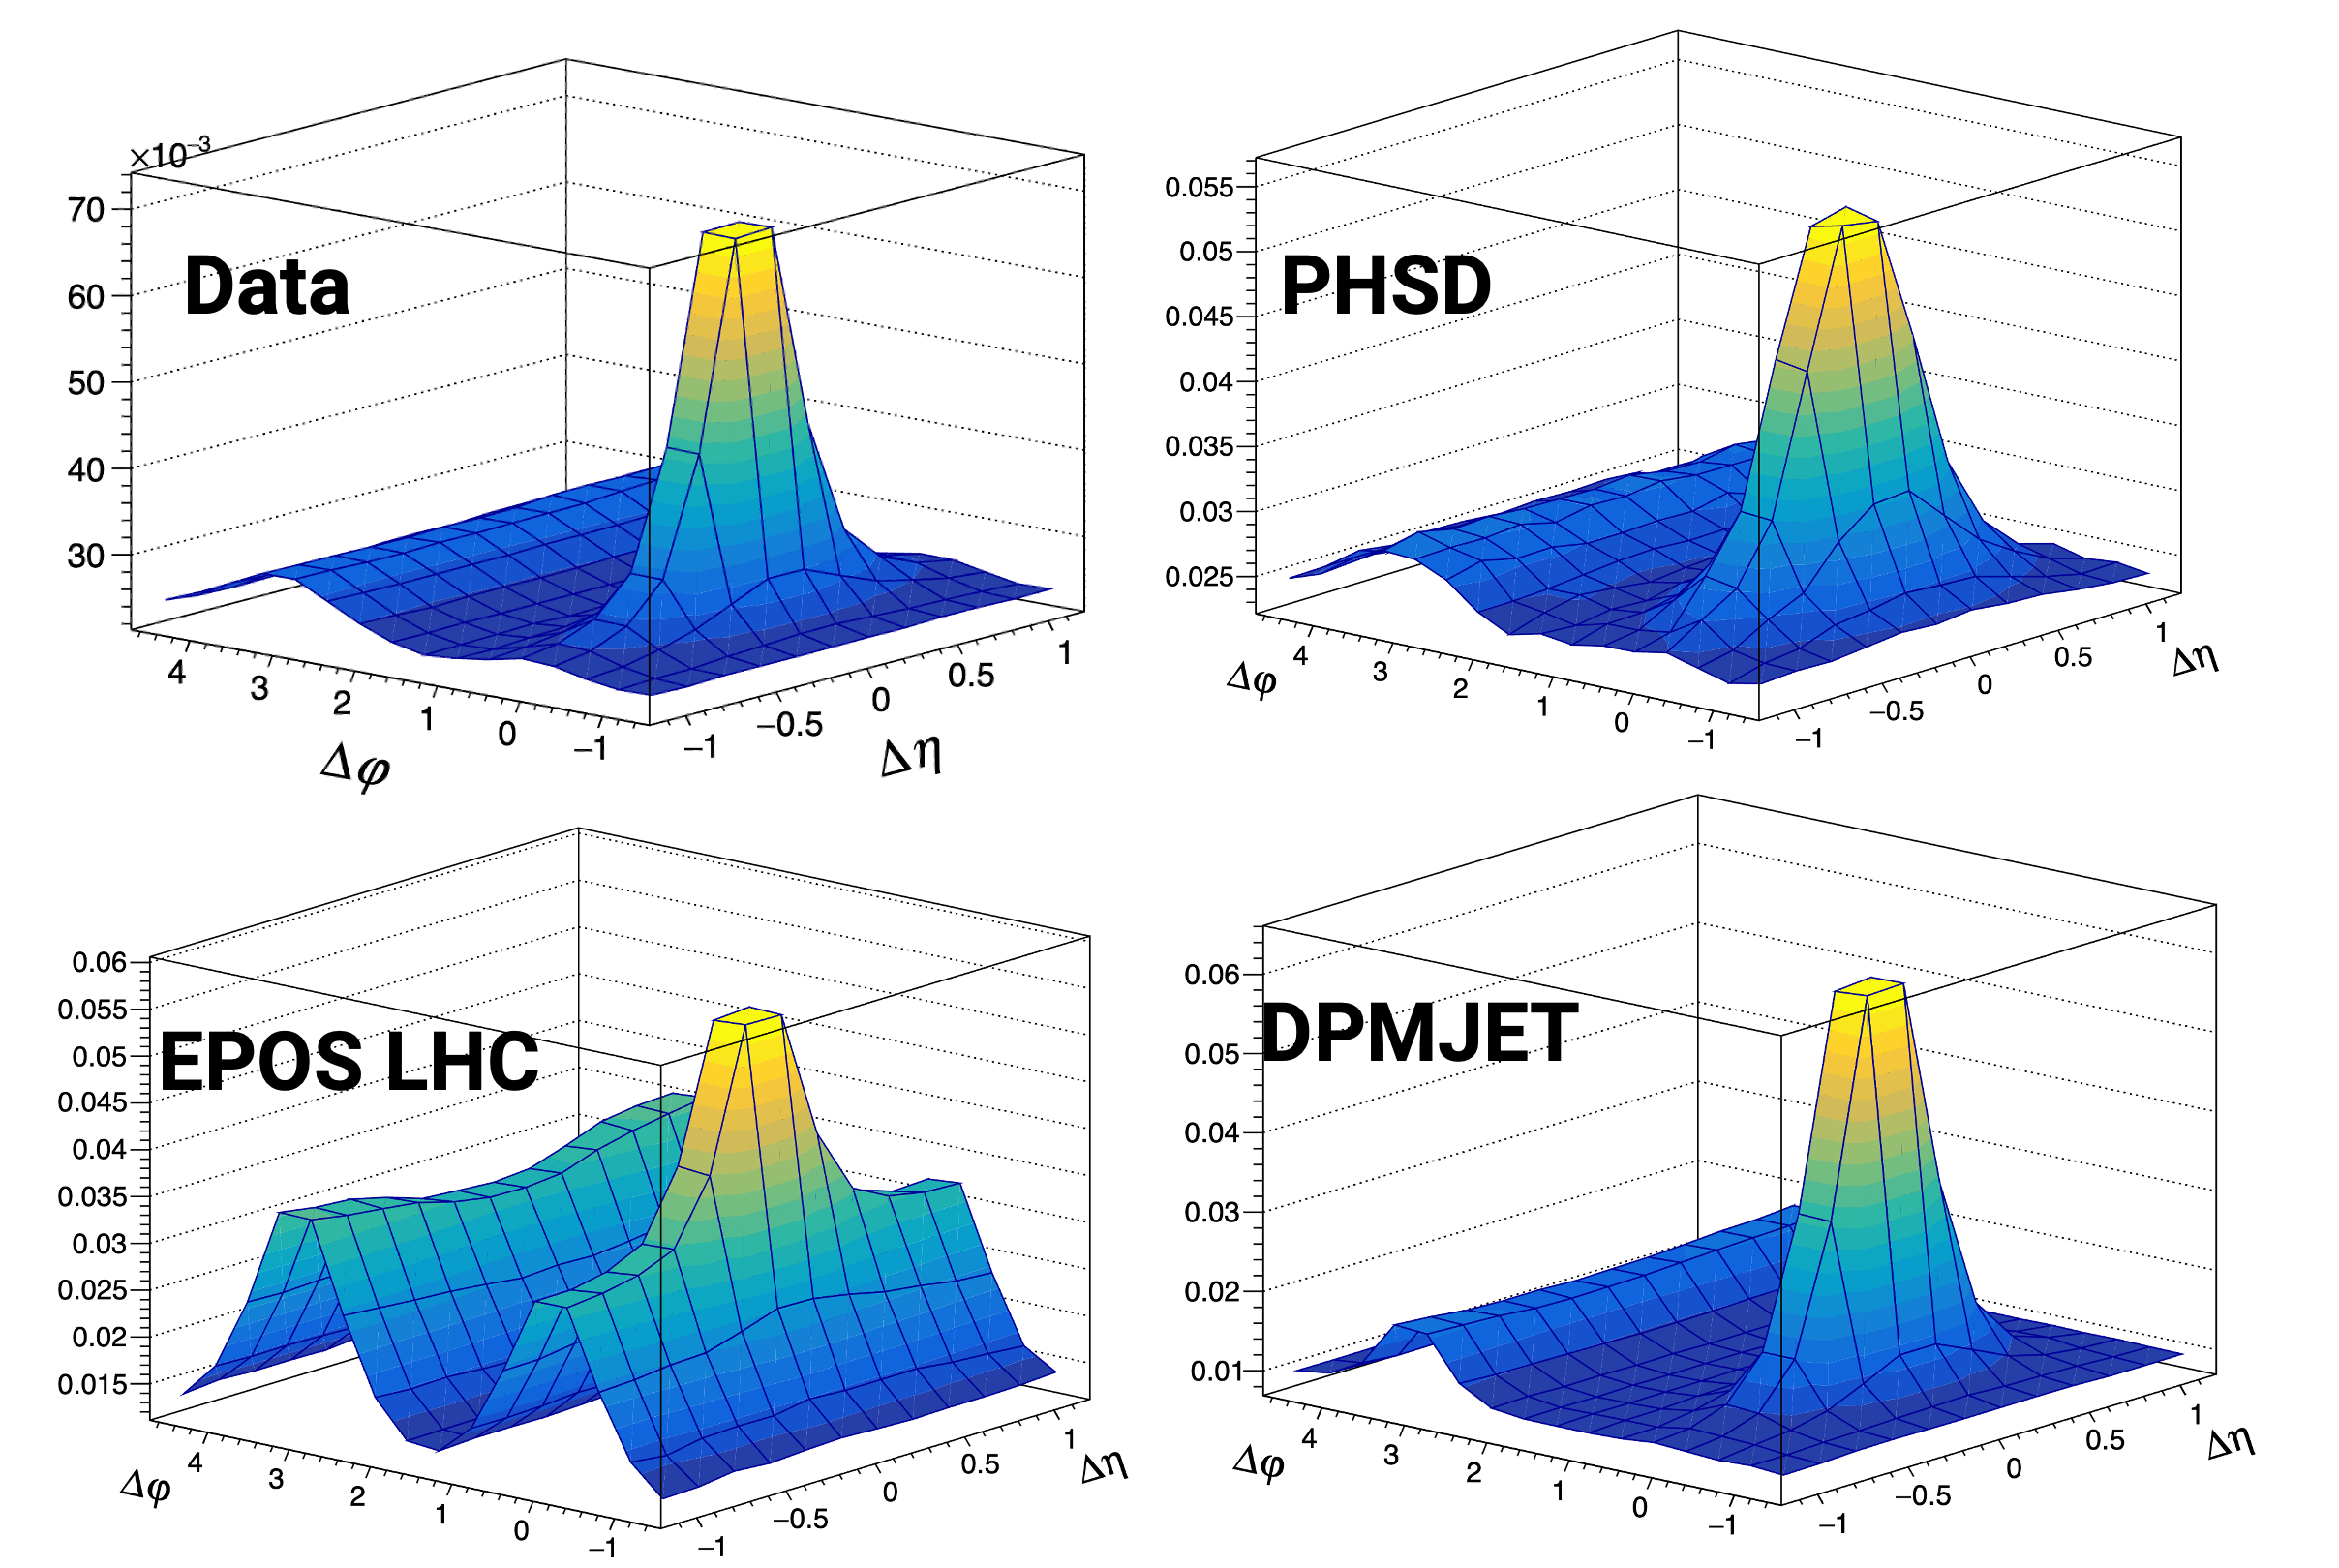
\includegraphics[width=\textwidth]{figures/results/h_h_2d_modelcomp.png}
\caption{The multiplicity-integrated per-trigger h-h 2D $\Delta\varphi\Delta\eta$ distributions in data and for each model within the $1.5 <$ \pt $< 2.5$ \GeVc associated momentum bin.}
\label{fig:h_h_2d_model}
\end{figure}

EPOS-LHC, on the other hand, has a very large flow component, well beyond that of the data. Additionally, the away-side jet region in EPOS-LHC appears to be completely washed-out. This is likely due to the hydrodynamic core of EPOS-LHC, which produces this collective flow at the expense of a loss of information from the initial hard-scatterings that produce the jets. As the Lund string density is greater on the away-side than the near-side, it is more likely for the strings in the away-side to form the core. This core, once formed, loses all of its correlations from the initial partonic scatterings, and thus the away-side jet correlation is destroyed. 

The yields and shape of the dihadron distribution from PHSD appears to match the data the best, with well-defined near- and away-side peaks, as well as a flow component that is similar to the data. The presence of this flow component is surprising, as PHSD is a microscopic transport model, where all of the constituent particles (partons, hadrons and strings) are treated as individual particles that interact with each other. For such a fundamental model to produce this collective behavior is a refreshing deviation from models that ``force'' this behavior through hydrodynamic means. However, the near-side peak appears to be lower in PHSD than in data, indicating that the description of jets within PHSD is not perfect.

\begin{figure}[ht]
\centering
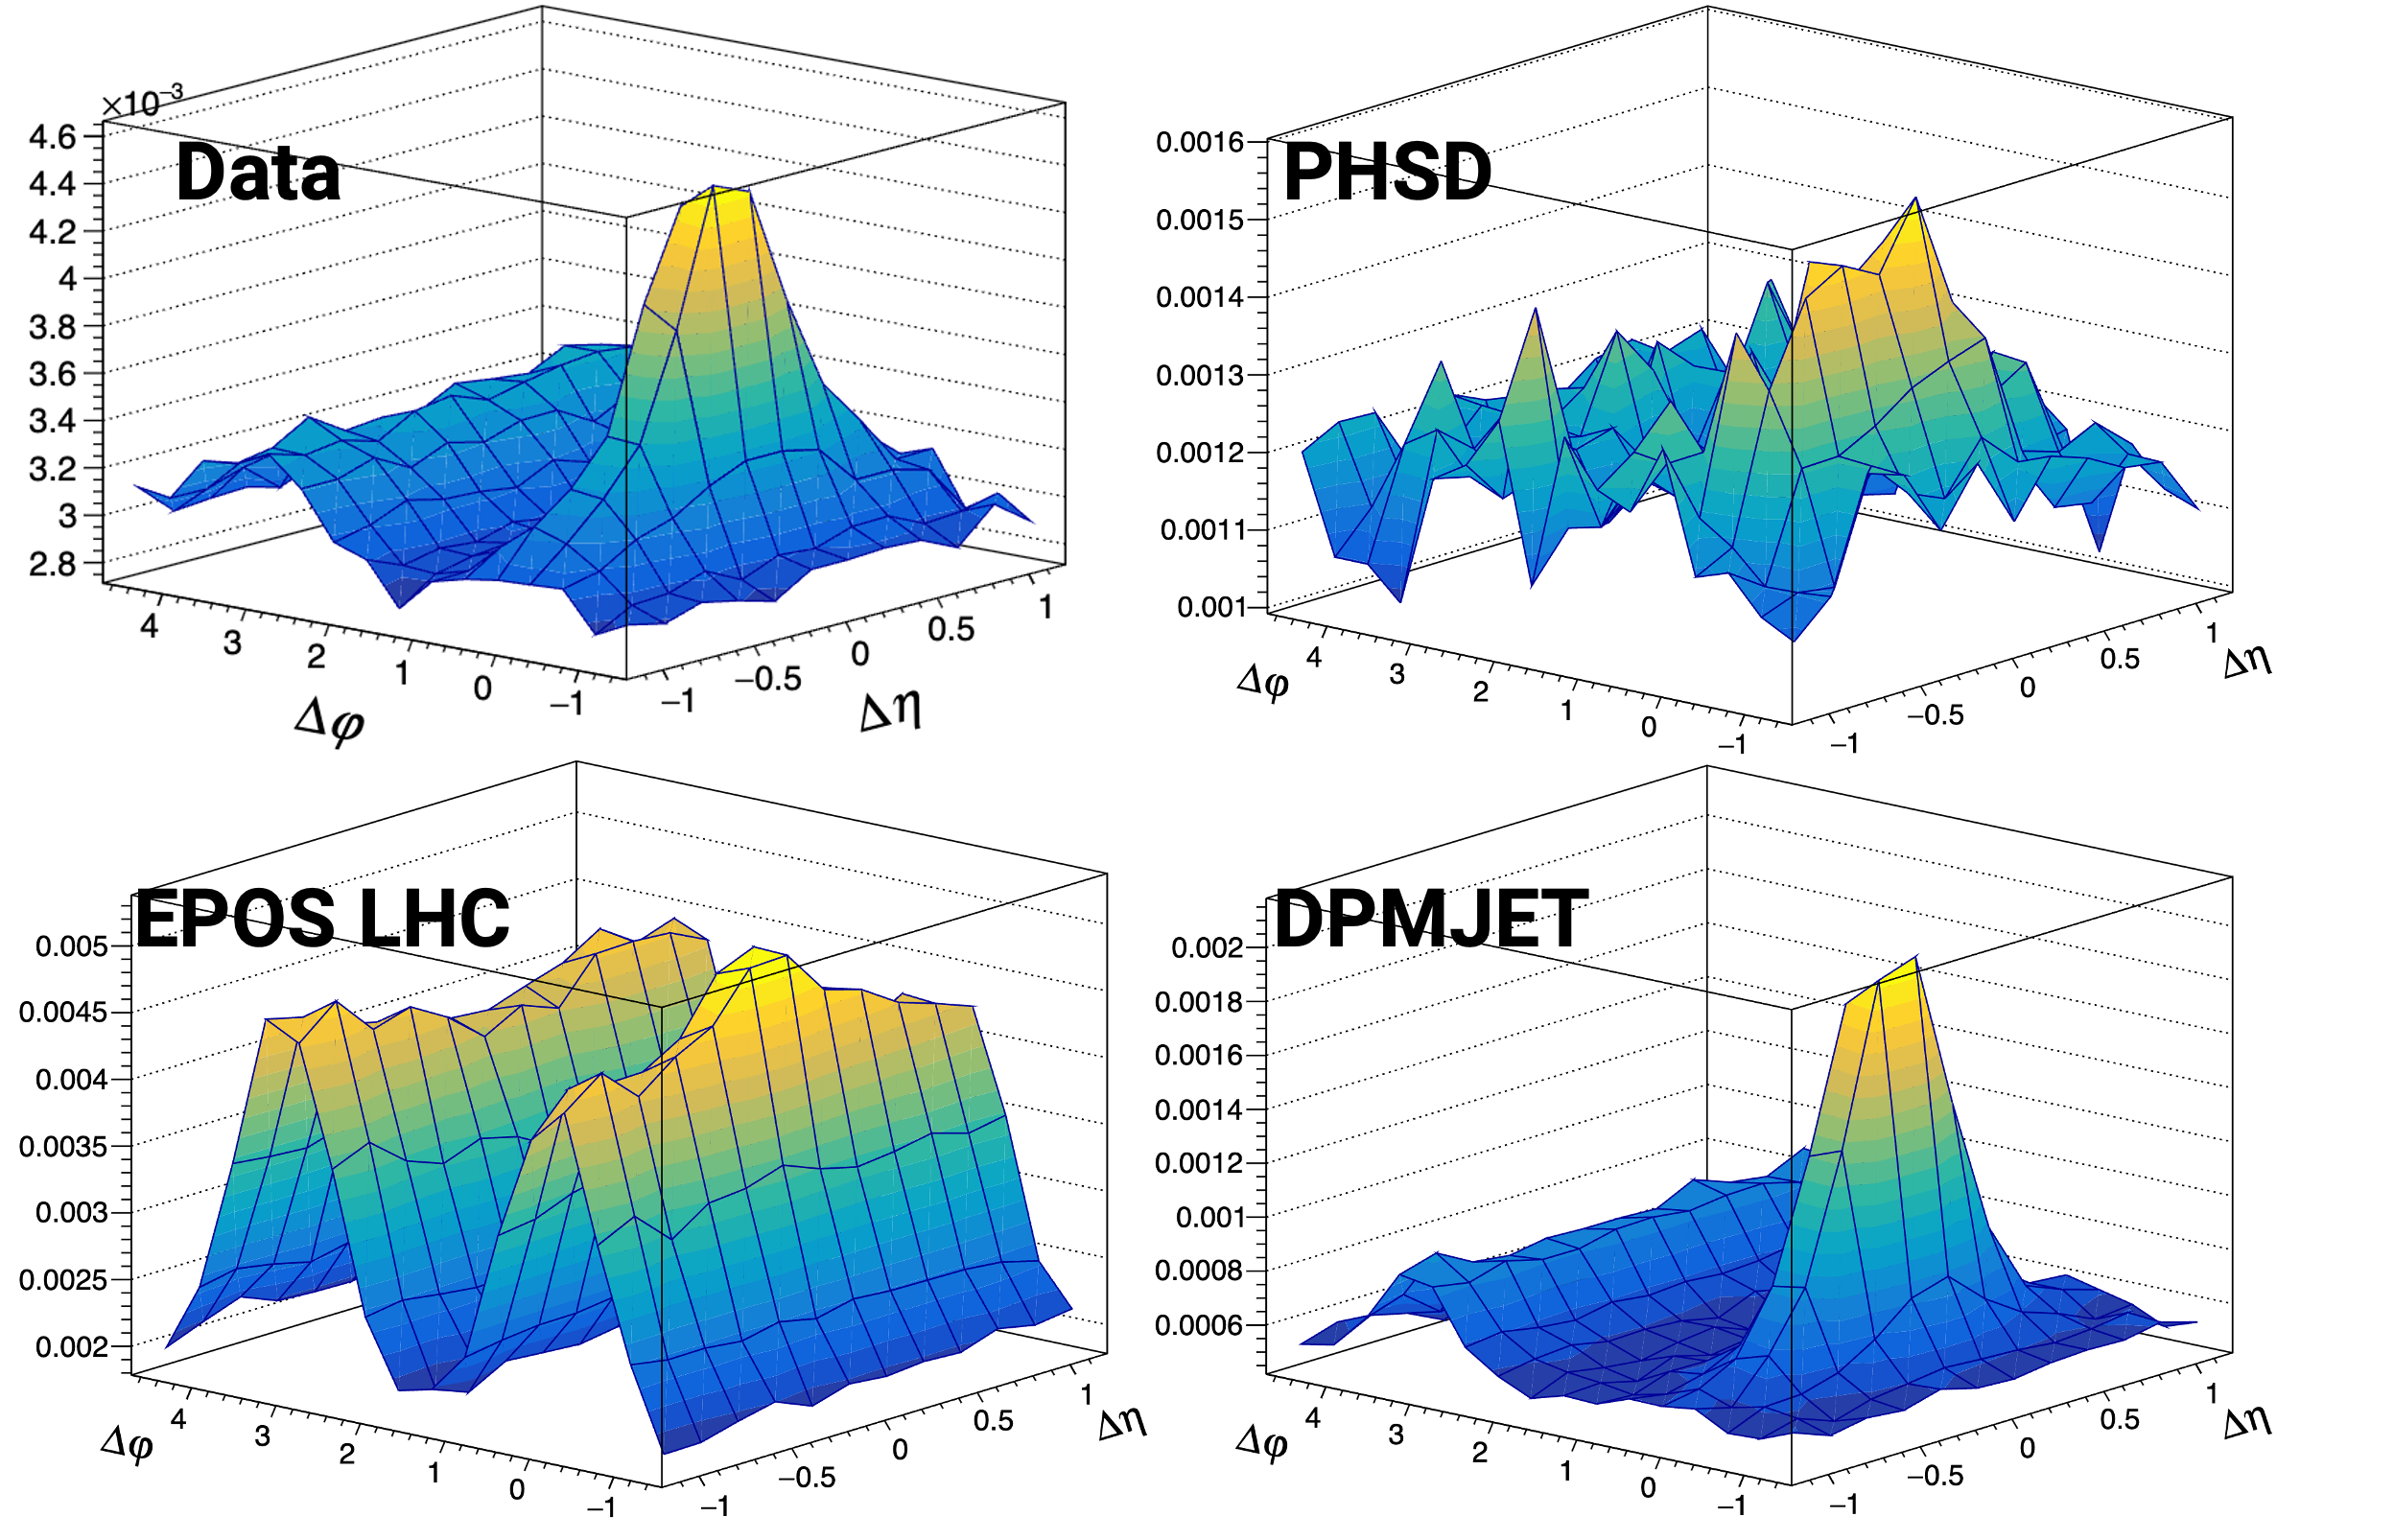
\includegraphics[width=\textwidth]{figures/results/h_lambda_2d_modelcomp.png}
\caption{The multiplicity-integrated per-trigger h-\lmb 2D $\Delta\varphi\Delta\eta$ distributions in data and for each model within the $1.5 <$ \pt $< 2.5$ \GeVc associated momentum bin.}
\label{fig:h_lambda_2d_model}
\end{figure}

For the h-$\Lambda$ distributions, the story is a bit different. DPMJET still overestimates the jet peaks and exhibits no flow, but the overall h-\lmb yield is now substantially lower than it is in data. The distribution from EPOS-LHC now shows very little signs of a near-side jet region, indicating that the production of $\Lambda$ baryons is coming almost \textit{entirely} from the hydrodynamic core. Still, the h-\lmb yields from EPOS are the closest to data, indicating that this core does a good job of making $\Lambda$ baryons (but a bad job at telling them where to go). The PHSD distribution is the most interesting, as it appears to be dominated by statistical fluctuations. As the PHSD yields are generated across 1.2 billion events (over twice as much as data and the other event generators), the conclusion is quite simple: PHSD does not produce enough $\Lambda$ baryons in events that have a trigger. This was investigated more thoroughly, and it was found that PHSD produces a factor of 10 less events with both a trigger hadron and a $\Lambda$ baryon than in data, shown in Figure~\ref{fig:phsd_woes}. In data, around 2\% of the event sample has both a trigger hadron and a $\Lambda$ baryon, whereas in PHSD this number is around 0.2\%. In order to generate the same number of h-\lmb pairs as seen in data, over 4 billion PHSD events would need to be generated, requiring a significant amount of computing resources.

\begin{figure}[ht]
\centering
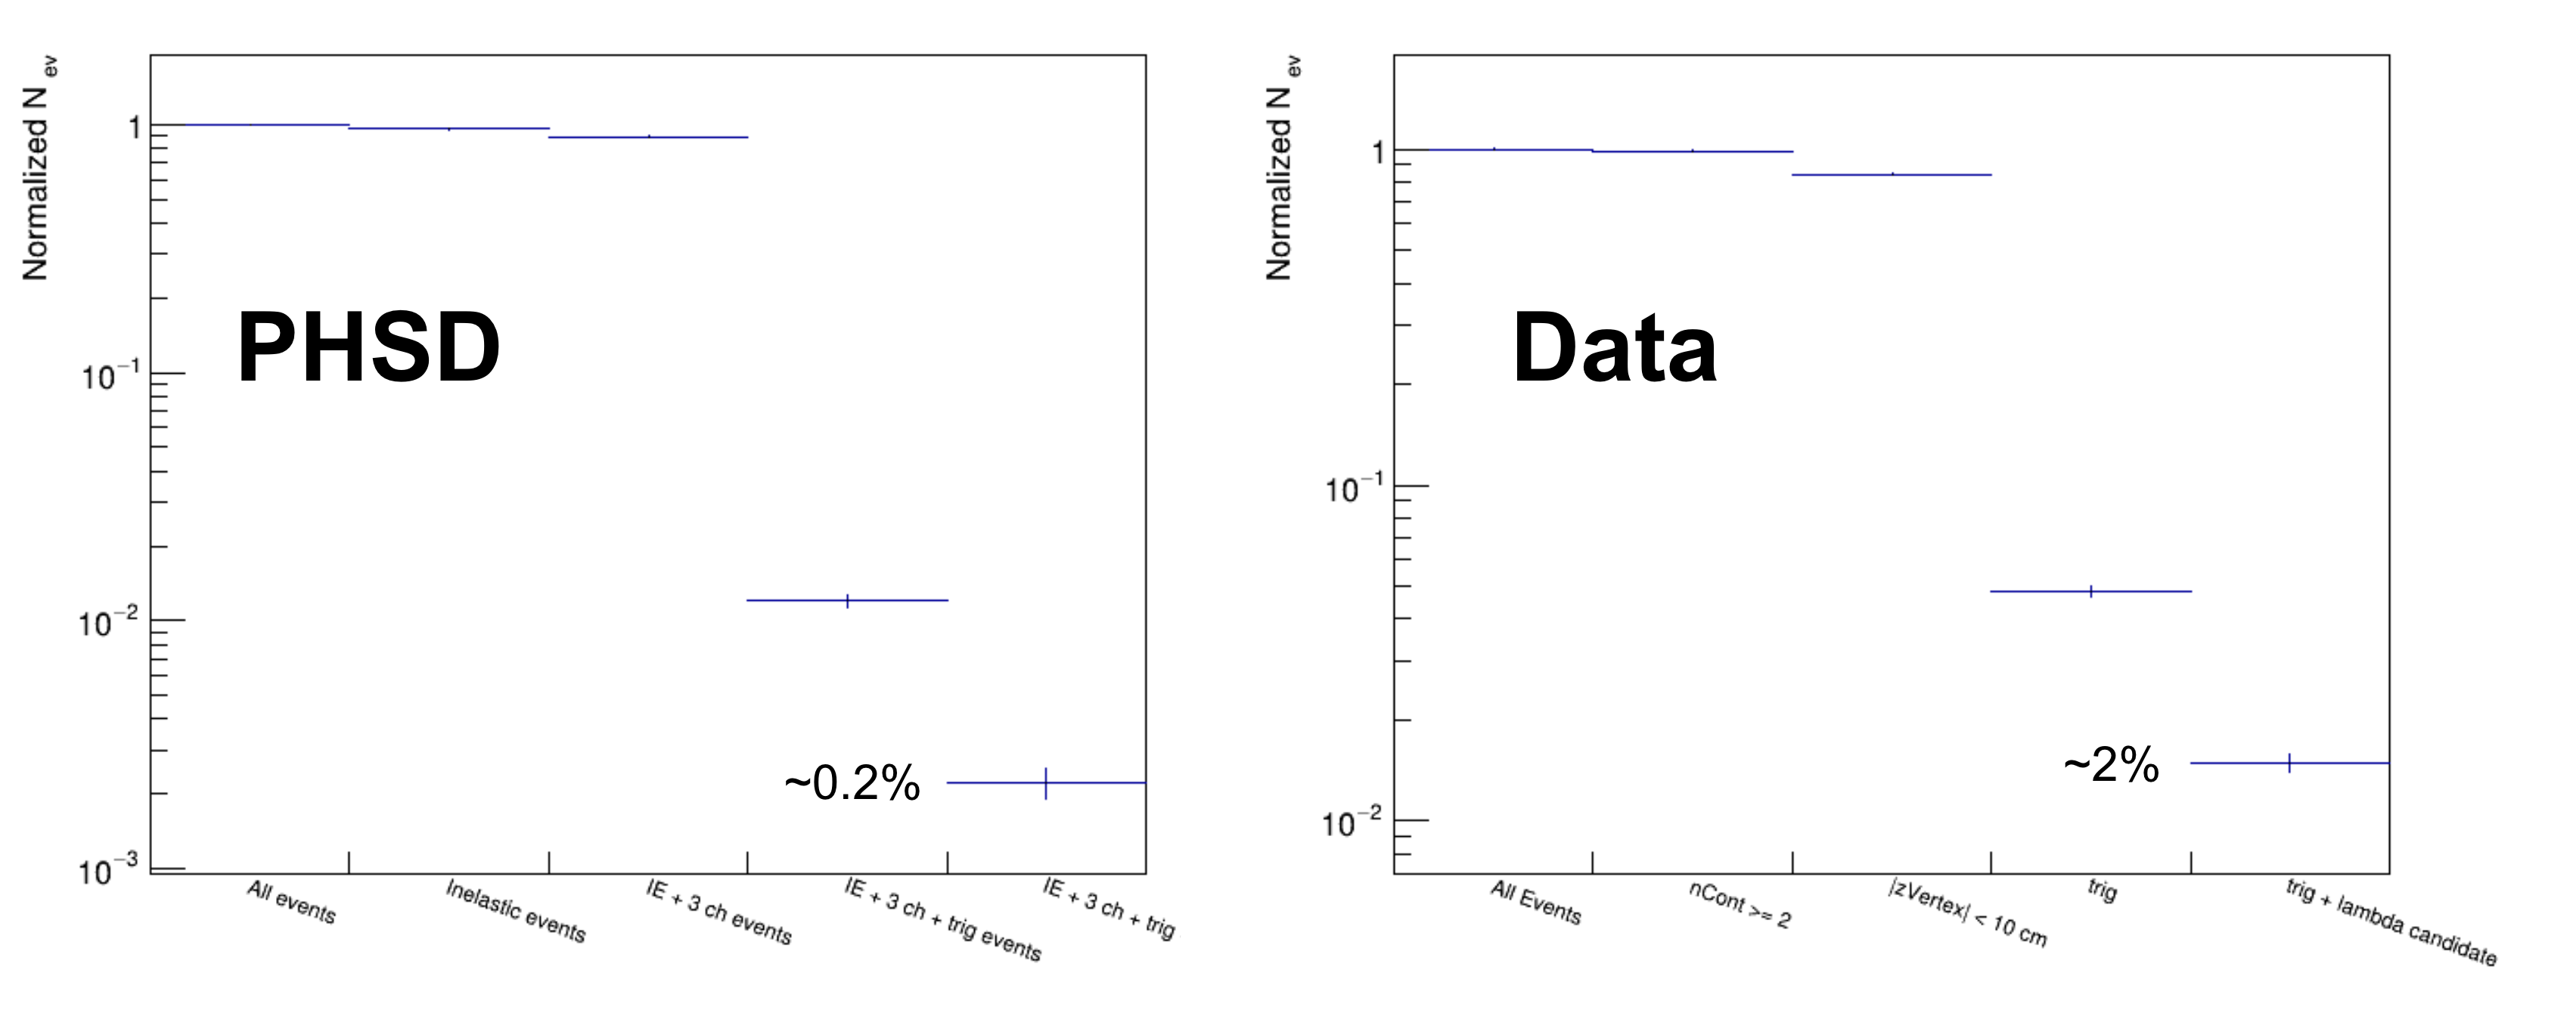
\includegraphics[width=\textwidth]{figures/results/phsd_woes.png}
\caption{The fraction of events that pass various selection criteria for PHSD (left) and data (right). The right-most bin in both distributions represents the fraction of events that contribute to the h-\lmb yield, which is 10 times lower in PHSD than it is in data.}
\label{fig:phsd_woes}
\end{figure}


\subsection{Per-trigger $\Delta\varphi$ distributions}
\label{sec:model_1d_correlations}

The $\Delta\varphi$ distributions generated by projecting the previous 2D distributions (Figures~\ref{fig:h_h_2d_model} and~\ref{fig:h_lambda_2d_model}) in the $|\Delta\eta| < 1.2$ range can be seen in Figures \ref{fig:h_lambda_1d_model} (h-$\Lambda$) and \ref{fig:h_h_1d_model} (h-h). While most of the distinct features for each model have already be addressed in terms of the 2D distributions, projecting onto $\Delta\varphi$ reveals a few more interesting properties. 

For the dihadron case, the shape of the $\Delta\varphi$ distribution in PHSD looks nearly \textit{identical} to the data. Even the yields are mostly correct, though the jet-like regions are slightly underestimated. The EPOS-LHC distribution is the perfect example of why it is important to first look at the 2D distribution \textit{before} projecting: there appears to be an away-side peak of comparable size to the near-side, but the 2D distribution reveals that this is entirely due to flow. Projecting onto $\Delta\varphi$ also makes it more clear that DPMJET does not accurately predict the UE contribution, which is nearly three times less than it is in data (0.12 vs. 0.29). The same can be said about the h-\lmb distributions, with the exception of PHSD. While the near-side peak is clearly visible, and its shape is somewhat similar to that in data, the away-side jet appears to have inexplicably vanished. Unfortunately the explanation for this is not as cut-and-dry as it was for EPOS-LHC, as PHSD has no hydrodynamic core. The investigation into this effect is still ongoing, and may be addressed in a future publication.

\begin{figure}[ht]
\centering
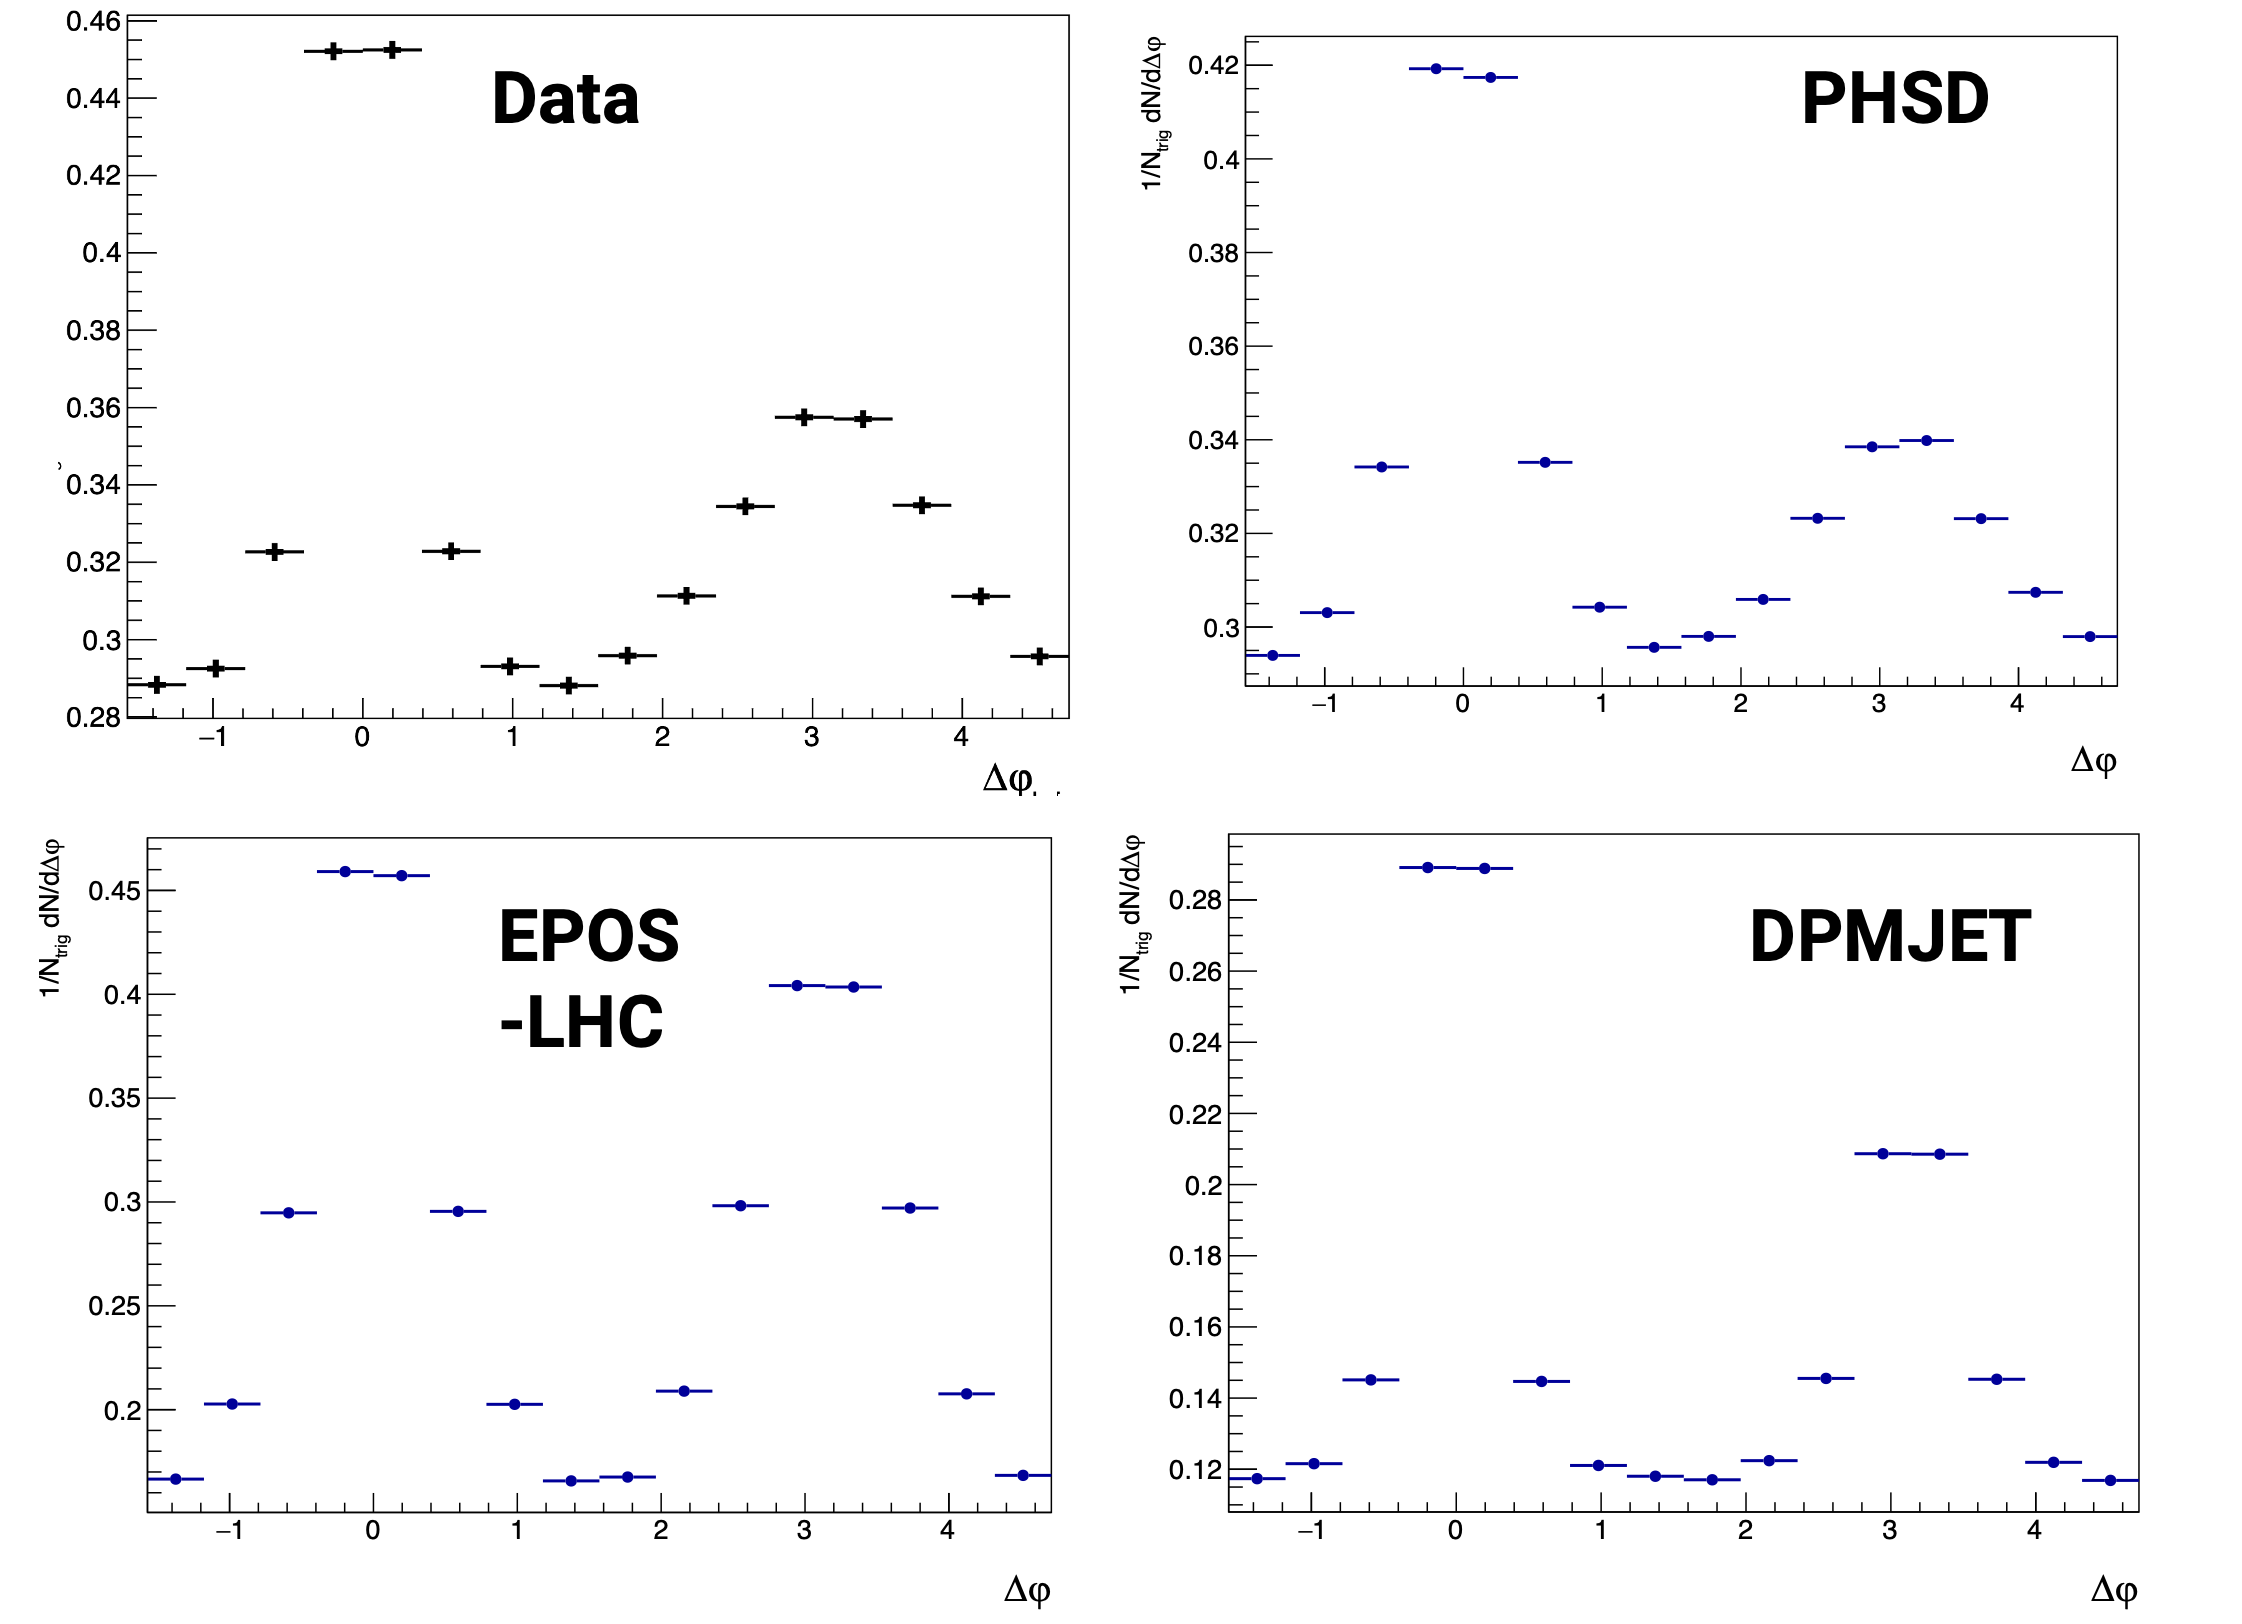
\includegraphics[width=\textwidth]{figures/results/h_h_1d_modelcomp.png}
\caption{The multiplicity-integrated per-trigger h-h $\Delta\varphi$ distributions in data and for each model within the $1.5 <$ \pt $< 2.5$ \GeVc associated momentum bin.}
\label{fig:h_h_1d_model}
\end{figure}

\begin{figure}[ht]
\centering
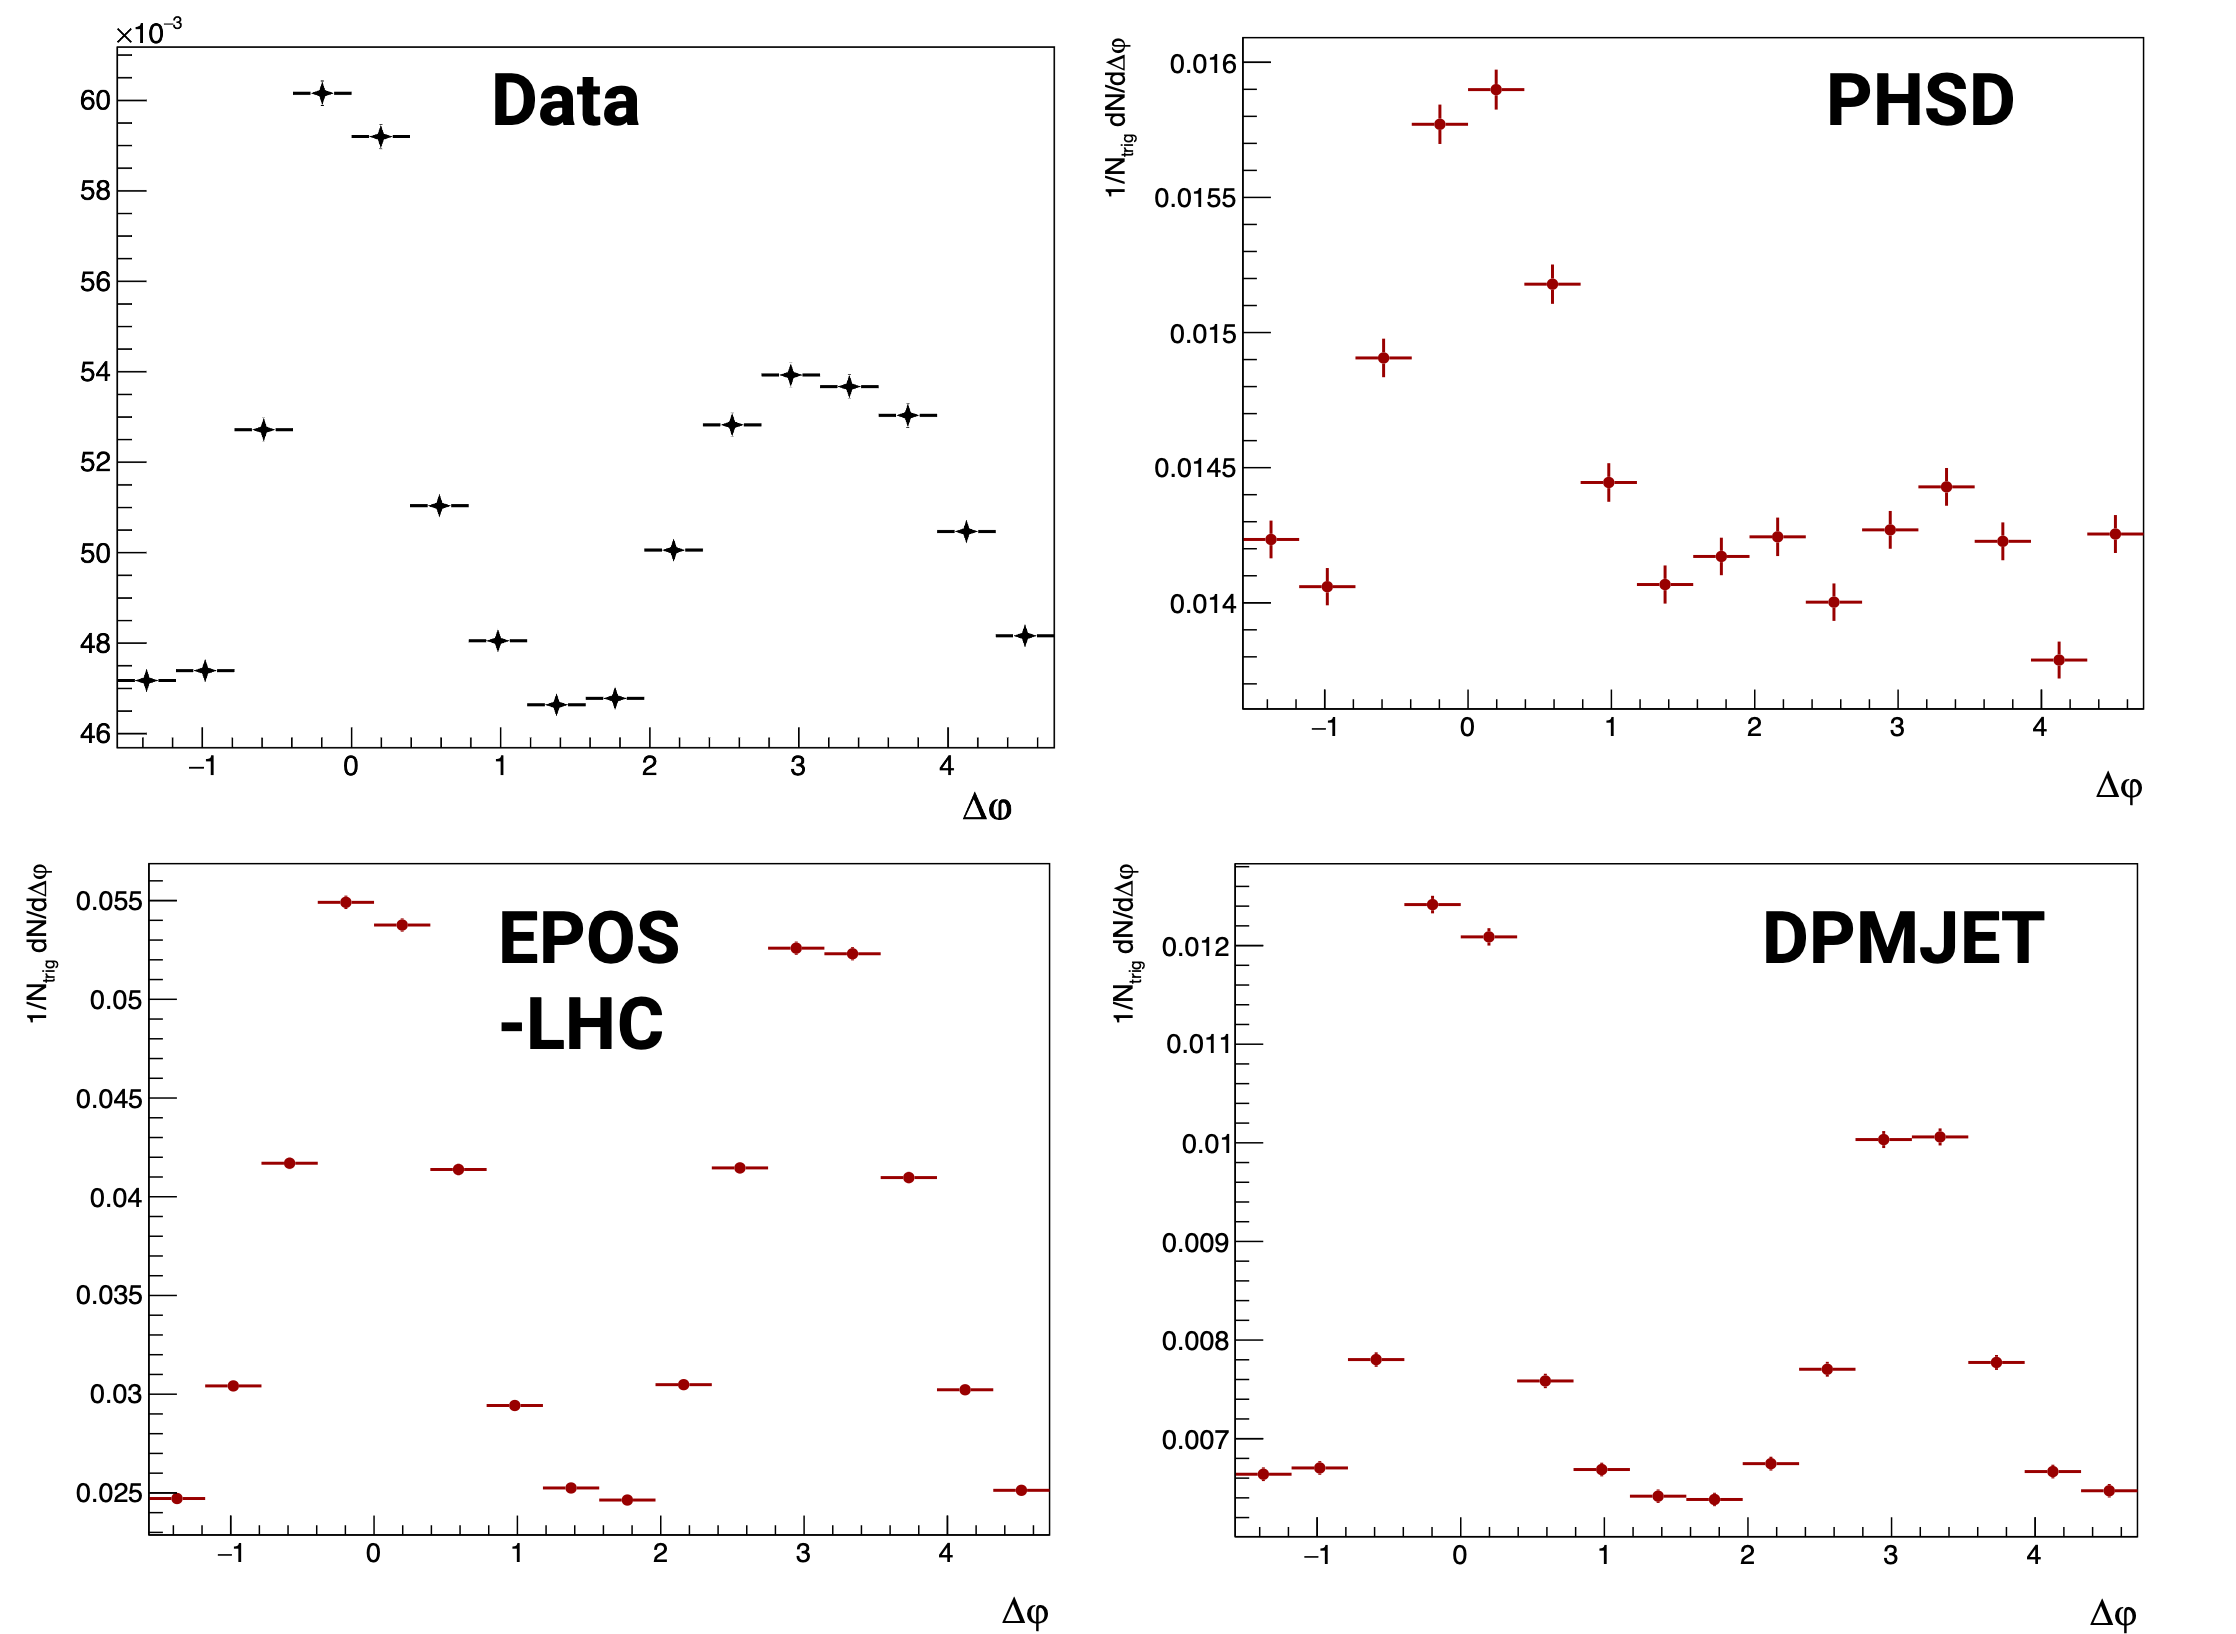
\includegraphics[width=\textwidth]{figures/results/h_lambda_1d_modelcomp.png}
\caption{The multiplicity-integrated per-trigger h-\lmb $\Delta\varphi$ distributions in data and for each model within the $1.5 <$ \pt $< 2.5$ \GeVc associated momentum bin.}
\label{fig:h_lambda_1d_model}
\end{figure}

Do to a lack of away-side jet peak in both EPOS-LHC and PHSD (and the overwhelming flow contribution to the $\Delta\varphi$ distribution in the case of EPOS-LHC), these models are excluded from the rest of the analysis. It is worth mentioning again, however, that PHSD shows promising initial results for dihadron correlation analyses. If the issues with the h-\lmb distributions can be resolved, PHSD looks like an excellent theoretical framework for these studies. 

The remainder of this section will focus on DPMJET, which, while clearly lacking in some areas, consistently exhibits a well-defined near- and away-side jet peak with a quantifiable UE contribution.

\subsubsection{Systematic uncertainties for DPMJET}
\label{sec:dpmjet_systematics}
While most of the systematic variations considered for this analysis are not relevant for model predictions, both the yield extraction procedure and width extraction procedure have systematic uncertainties that should be taken into account. As such, a table of the systematic uncertainties for the DPMJET model predictions in each multiplicity bin is provided in Tables \ref{dpmjet_systematics_table_lambda} (h-$\Lambda$) and \ref{dpmjet_systematics_table_h} (h-h). As these uncertainties are independent of associated \pt, only the 1.5 - 2.5 \GeVc associated momentum bin are given. 

\begin{table}[ht]
\centering
\begin{tabular}{|c||c|c|c|c|c|c|}
\hline
Mult. Bin & NS width & AS width & NS yield & AS yield & UE yield  \\
\hline
0-20\% &  1.0 & 0.9 & 0.6 & 0.9 & 0.8  \\
20-50\% &  1.0 & 1.6 & 0.7 & 0.8 & 0.9  \\
50-80\% &  0.4 & 1.0 & 0.6 & 0.8 & 0.6  \\
\hline
\end{tabular}
\caption{The total systematic uncertainties associated with the various width and yield extraction procedures in DPMJet for the h-$\Lambda$ distributions.}
\label{dpmjet_systematics_table_lambda}
\end{table}

\begin{table}[ht]
\centering
\begin{tabular}{|c||c|c|c|c|c|c|}
\hline
Mult. Bin & NS width & AS width & NS yield & AS yield & UE yield \\
\hline
0-20\% &  0.9 & 1.2 & 1.0 & 0.7 & 0.9 & 0.0 \\
20-50\% &  0.7 & 1.2 & 1.0 & 0.7 & 0.7 & 0.0 \\
50-80\% &  0.3 & 1.3 & 0.6 & 0.7 & 0.6 & 0.0 \\
\hline
\end{tabular}
\caption{The total systematic uncertainties associated with the various width and yield extraction procedures in DPMJet for the h-h distributions.}
\label{dpmjet_systematics_table_h}
\end{table}

\subsection{Per-trigger jet-like yields and jet widths}
\label{sec:pairwise_yields_modelcomp}

A comparison between the per-trigger jet-like yields in data and the same yields predicted by DPMJET for each associated \pt range as a function of multiplicity can be seen in Figure \ref{fig:pairwise_yield_model}. Straight line fits of the data are shown as dashed lines. The same yields obtained using DPMJET shown as bands representing their systematic uncertainty, with a ratio to the data presented in the bottom panel. A dashed line at unity is drawn to help better visualize the deviations between data and the model.

\begin{figure}[h!]
\centering
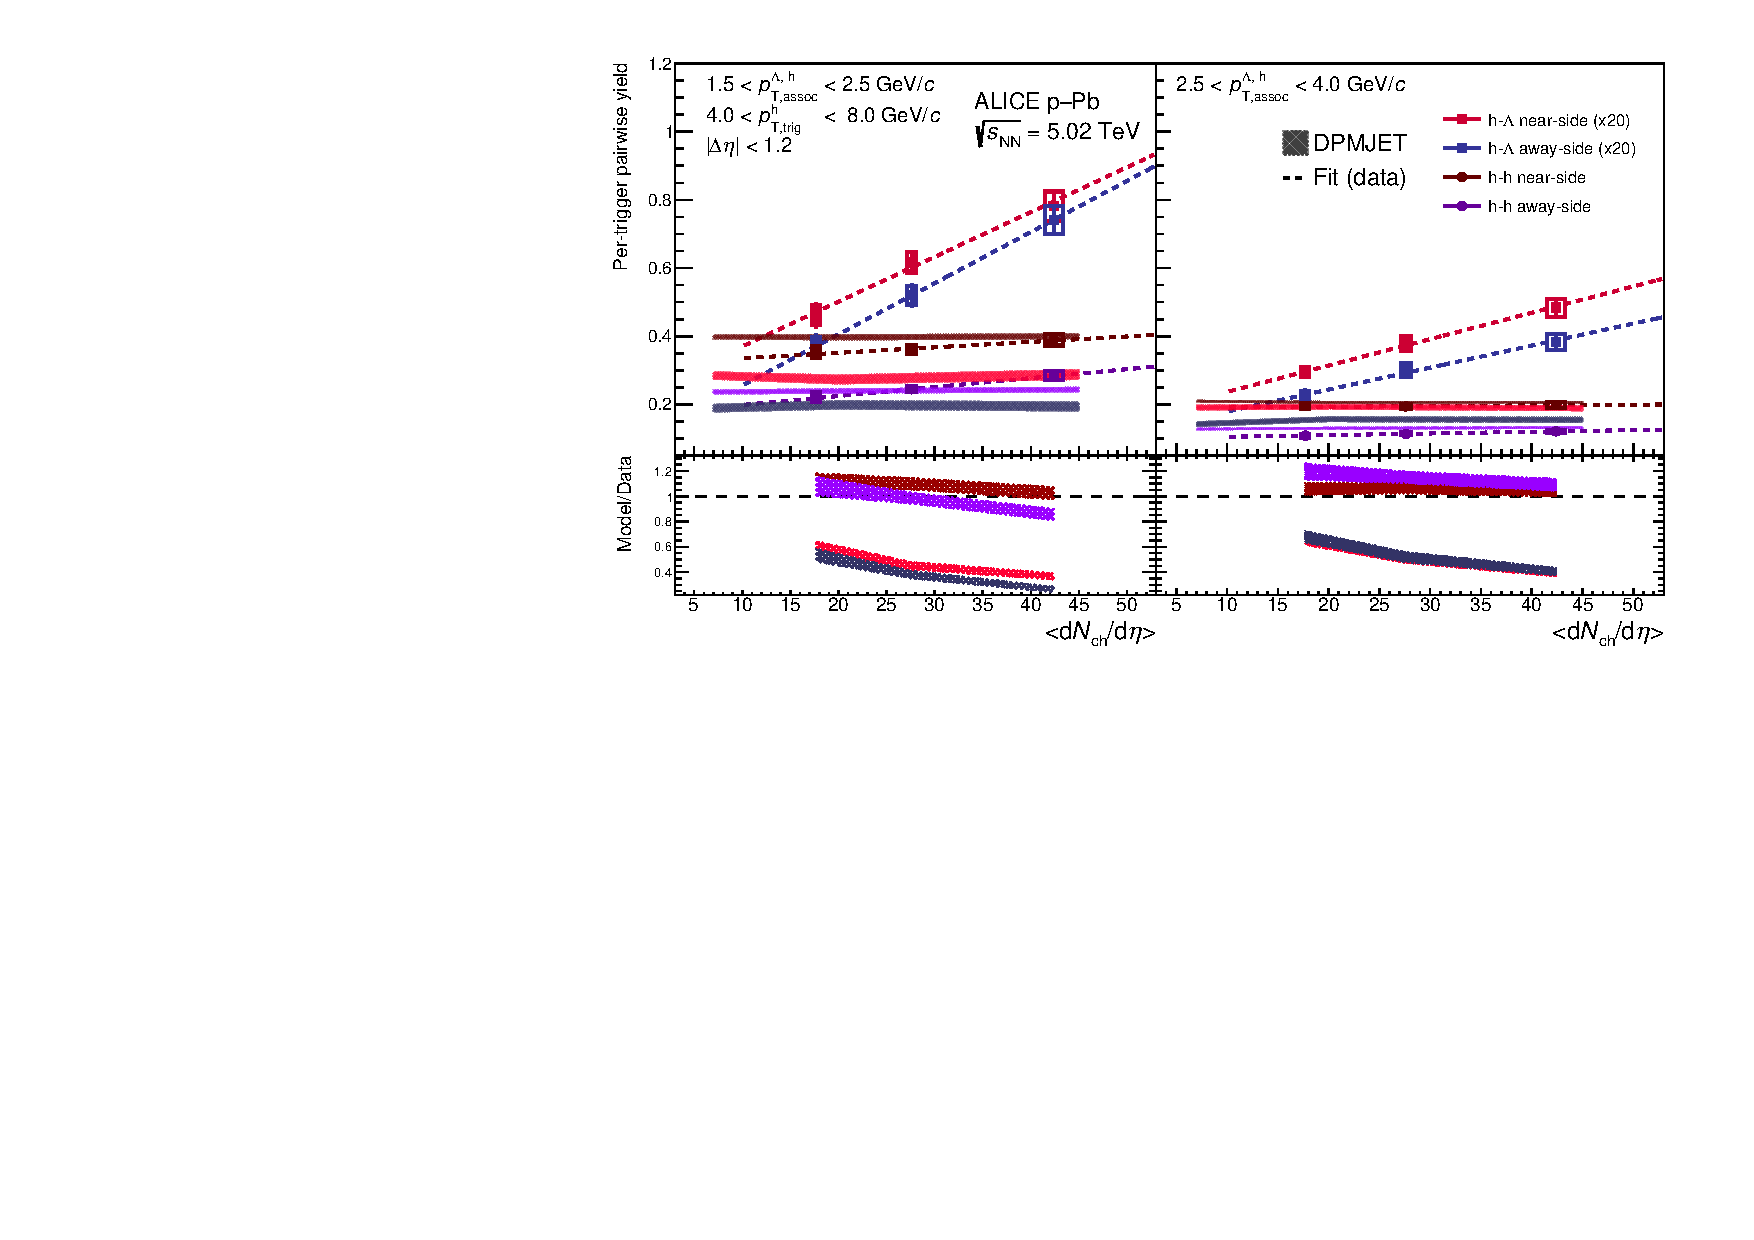
\includegraphics[width=\textwidth]{figures/results/final_pairwise_plot_new_x_axis_model_ratio.pdf}
\caption{The per-trigger pair-wise yields $Y_{\text{near}}, Y_{\text{away}}$ as a function of charged particle multiplicity for the h-$\Lambda$ (square markers) and h-h (circle markers) correlations in the lower (left) and higher (right) associated \pt ranges. The statistical (systematic) uncertainties are shown as vertical lines (boxes), and a first order polynomial fit to the data is shown as a dashed line. The same yields predicted by DPMJET are also shown as shaded bands, with the width of the band representing the systematic uncertainty on the model. The ratio of the model to the data is shown in the bottom panel, along with a dashed line drawn at unity.}
\label{fig:pairwise_yield_model}
\end{figure}

The per-trigger near- and away-side yields predicted by DPMJET are mostly consistent with data in the dihadron case. This can be seen in the model/data ratio, with both the near- and away-side ratios remaining close to unity across the entire multiplicity range. The h-$\Lambda$ yields, however, are not well described by the model. Both the near- and away-side h-$\Lambda$ yields predicted by DPMJET are lower than data by around a factor of two across the entire multiplicity range in both momentum ranges, and there is no significant increase in these yields as a function of multiplicity. This is not unexpected: as mentioned in the previous section, DPMJET does not appear to exhibit \textit{any} medium effects, and thus any possible enhancement in the production of $\Lambda$ baryons due to the formation of a QGP is not present.

A comparison between DPMJET and data for the near- and away-side jet widths for each associated \pt range as a function of multiplicity is also presented in Figure \ref{fig:jet_widths_model}. Again, straight line fits of the data are shown as dashed lines, and the widths obtained using DPMJET are shown as bands representing their systematic uncertainty. A model/data ratio is also given in the bottom panel, with a dashed line drawn at unity.


\begin{figure}[h!]
\centering
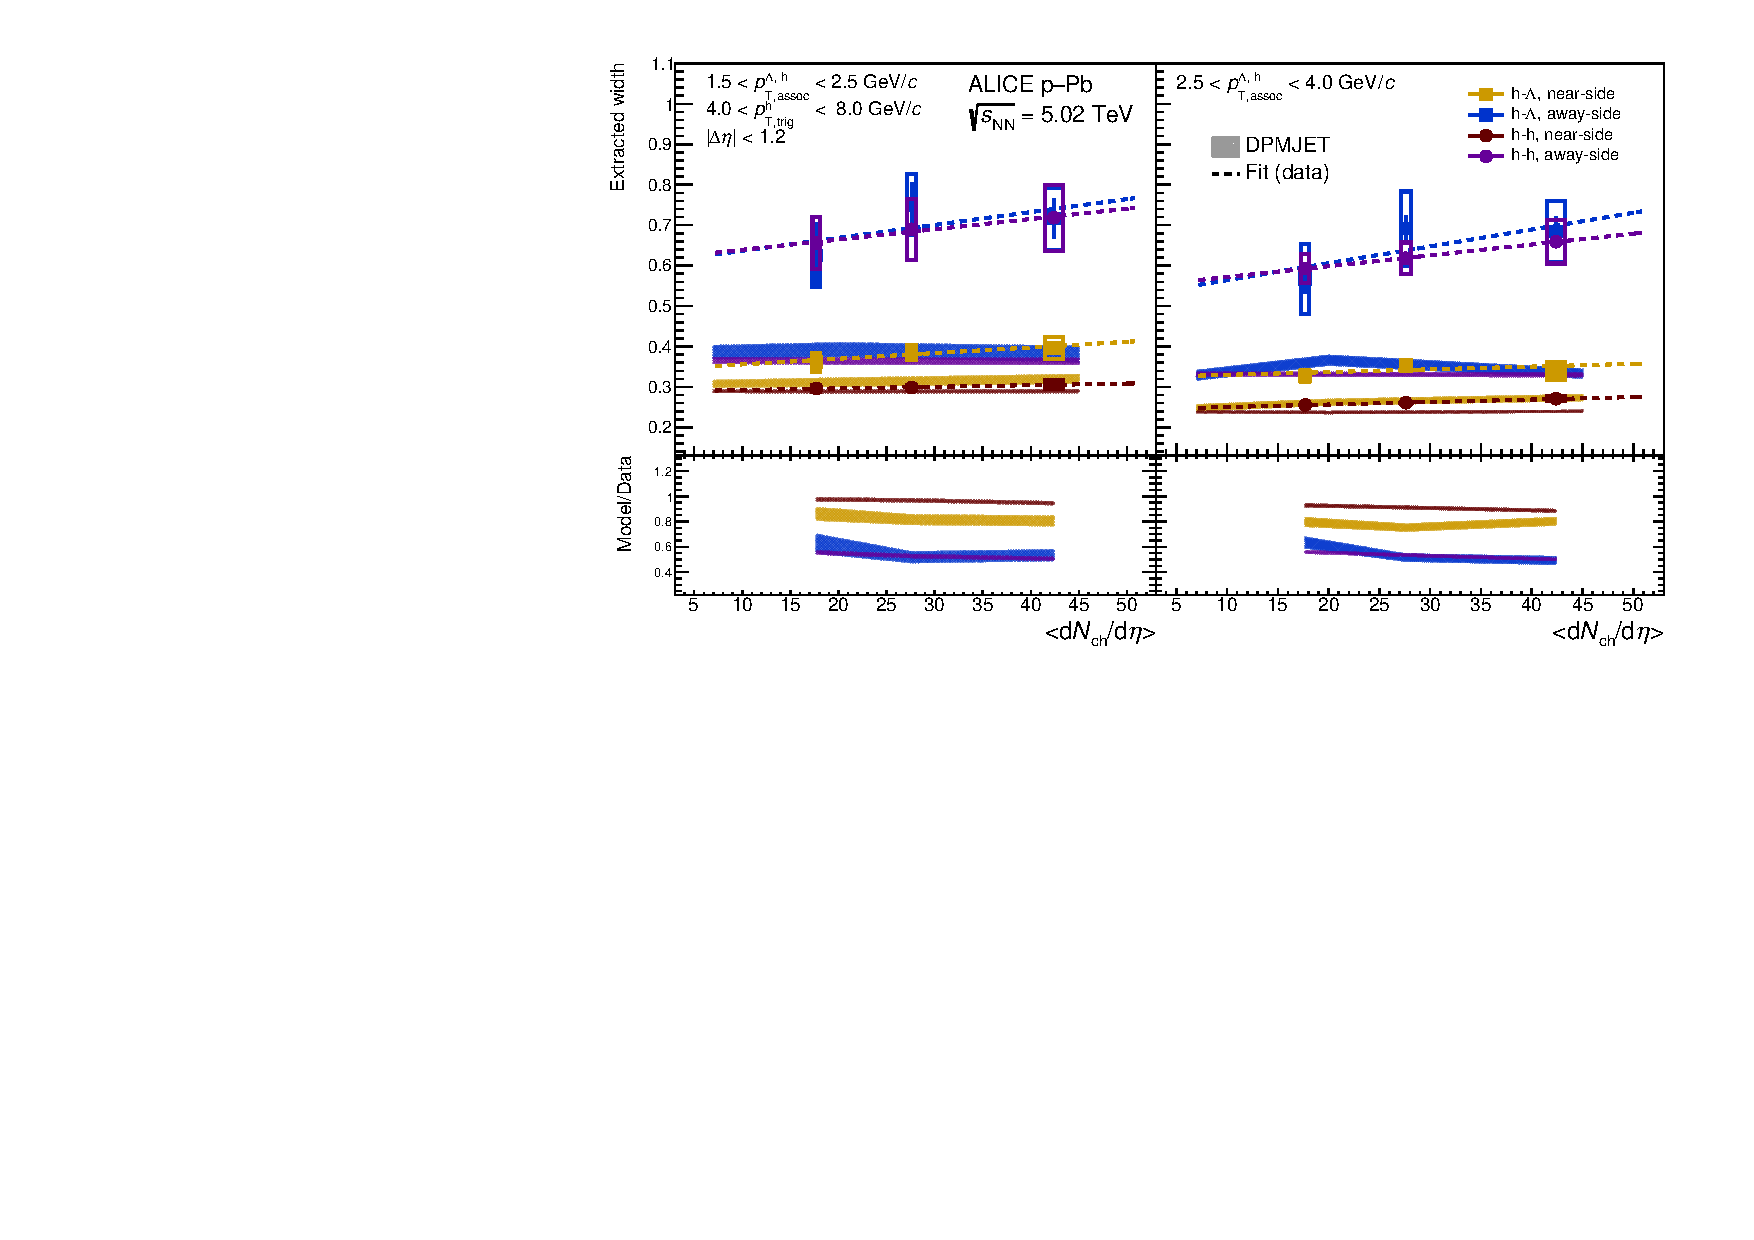
\includegraphics[width=\textwidth]{figures/results/final_width_plot_new_x_axis_model_ratio.pdf}
\caption{The h-$\Lambda$ and h-h near- and away-side peak widths shown as a function of multiplicity for both associated momentum ranges, along with a straight-line fit to the data. The statistical (systematic) uncertainties are shown as vertical lines (boxes). The ratios predicted by DPMJET are also presented as shaded bands, with the width of the band represending the systematic uncertainty on the model. The ratio of the model to the data is presented in the bottom panel, along with a dashed line drawn at unity.}
\label{fig:jet_widths_model}
\end{figure}

For the h-h near-side widths, DPMJET describes the data well across both momentum ranges, with a $<5 (10)$\%  deviation from data seen in the lower (higher) momentum range. DPMJET also predicts the h-$\Lambda$ near-side width to be larger than the h-h width, though the values of the h-$\Lambda$ widths are much lower than they are in data. An alternative explanation to the one given in Section~\ref{sec:jet_like_yield_width} for these differences between the near-side widths is that they could be due to the presence of gluon jets, which are generally more wide than quark jets ~\cite{GluonJet1} and exhibit an increased production of $\Lambda$ baryons ~\cite{GluonJet2}. As DPMJET includes both quark and gluon jets, it is possible that the predicted differences between the h-$\Lambda$ and h-h near- and away-side peak widths are due to this effect. DPMJET also under-predicts both the h-$\Lambda$ and h-h away-side widths by around 40\% across both momentum ranges. As the DPMJET model does not include any medium effects, this suggests that the away-side peak widths in data are possibly ``broadened'' by jet-medium interactions. However, the larger uncertainties on the away-side widths prevent the exclusion of flat behavior with respect to multiplicity (i.e. increasing medium size), as the slopes are all consistent with zero within uncertainties.

\subsection{Per-trigger yield ratios}
\label{sec:ratios_modelcomp}

 A comparison between the per-trigger yield ratios in data and using DPMJET for each \pt bin as a function of multiplicity are shown in Figure~\ref{fig:lambda_hadron_ratio_model}. As before, straight line fits of the data are shown as dashed lines, and the widths obtained using DPMJET are shown as bands representing their systematic uncertainty. A model/data ratio is also presented in the bottom panel, with a dashed line drawn at unity.

\begin{figure}[h!]
\centering
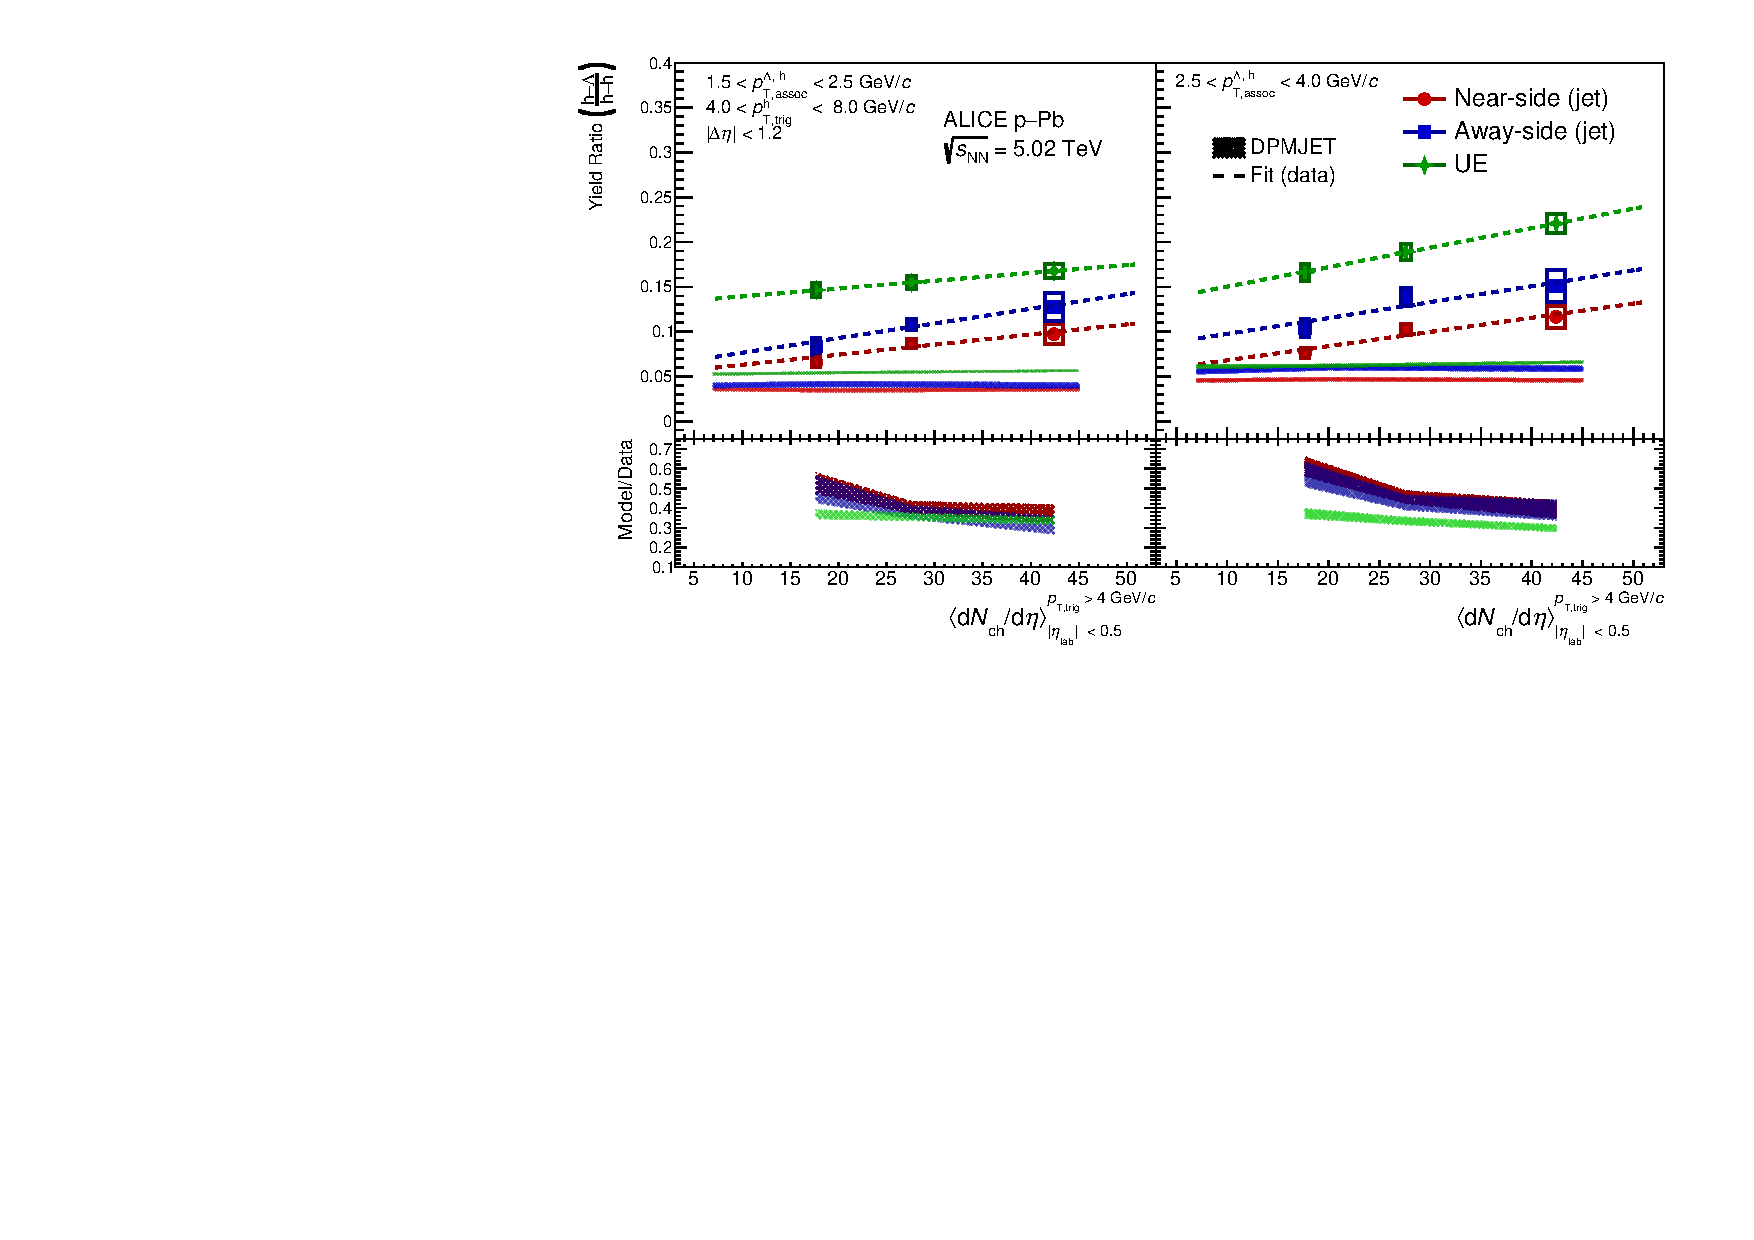
\includegraphics[width=\textwidth]{figures/results/final_lambda_hadron_ratio_plot_new_x_axis_model_ratio.pdf}
\caption{The per-trigger pair-wise yield ratios $R_{i}^{\Lambda/h} \equiv Y_{i}^{h-\Lambda}$/$Y_{i}^{h-h}$ ($i$ = near-side, away-side, UE) as a function of multiplicity in the lower (left) and higher (right) associated momentum ranges. The statistical (systematic) uncertainties are shown as vertical lines (boxes). The ratios predicted by DPMJET are also presented as shaded bands, with the width of the band represending the systematic uncertainty on the model. The ratio of the model to the data is presented in the bottom panel.}
\label{fig:lambda_hadron_ratio_model}
\end{figure}

Unsuprisingly (given the discussions in Section~\ref{sec:model_1d_correlations}), DPMJET underpredicts these ratios across the entire multiplicity range for both \pt bins. However, the straight line fits to the data appear like they may converge to DPMJET at sufficiently low multiplicities, indicating that DPMJET may be able to describe the magnitudes of these ratios in lower multiplicity pp collisions. This is not unexpected, as these lower multiplicity collisions are mostly described by the Lund string component of DPMJET, which is notorious for describing many features of these smaller collision systems~\cite{Pythia}.  While DPMJET is not able to predict any of the multiplicity-dependent behavior seen in data, it is able to produce the observed ordering in the ratios (UE > away-side > near-side), which indicates that the dominating production mechanisms for $\Lambda$ baryons within DPMJET come from the softer, less-correlated DPM processes.

\section{Comparison with the $\phi(1020)$}
\label{sec:phi_comparison}

The $\phi(1020)$ meson's net strangeness $|S|$ is equal to zero. Despite this, it has been observed to exhibit a similar enhancement in production as a function of multiplicity as other hadrons with non-zero strangeness ~\cite{PhiEnhancement}. Due to their similar masses ($\Delta M < 100$ \MeVmass), the $\phi(1020)$ is an excellect candidate to compare directly with the $\Lambda$ in order to better understand the differences between open ($|S| \neq 0$) and hidden ($|S| = 0$) strange hadron production. Using previously published results on $\phi(1020)$ production in and out-of jets in \pPb collisions at $\sqrt{s_{\text{NN}}} = 5.02$ \TeV ~\cite{JustinPaper} (shown in Figure~\ref{fig:justin_plots}), the per-trigger pair-wise yield ratios $R_{i}^{\Lambda/\phi} \equiv Y_{i}^{h-\Lambda}/Y_{i}^{h-\phi}$ ($i$ = near-side, away-side, UE) can be measured as a function of multiplicity. These ratios are presented in Figure \ref{fig:lambda_phi_ratio} for both the lower and higher associated \pt ranges. Again, straight line fits to the data are shown as a dashed lines, with the slopes and corresponding errors reported in Table \ref{tab:lambda_phi_slopes}. The same ratios predicted by DPMJET are also presented, with a ratio to the data presented in the bottom panel.

\begin{figure}[h!]
\centering
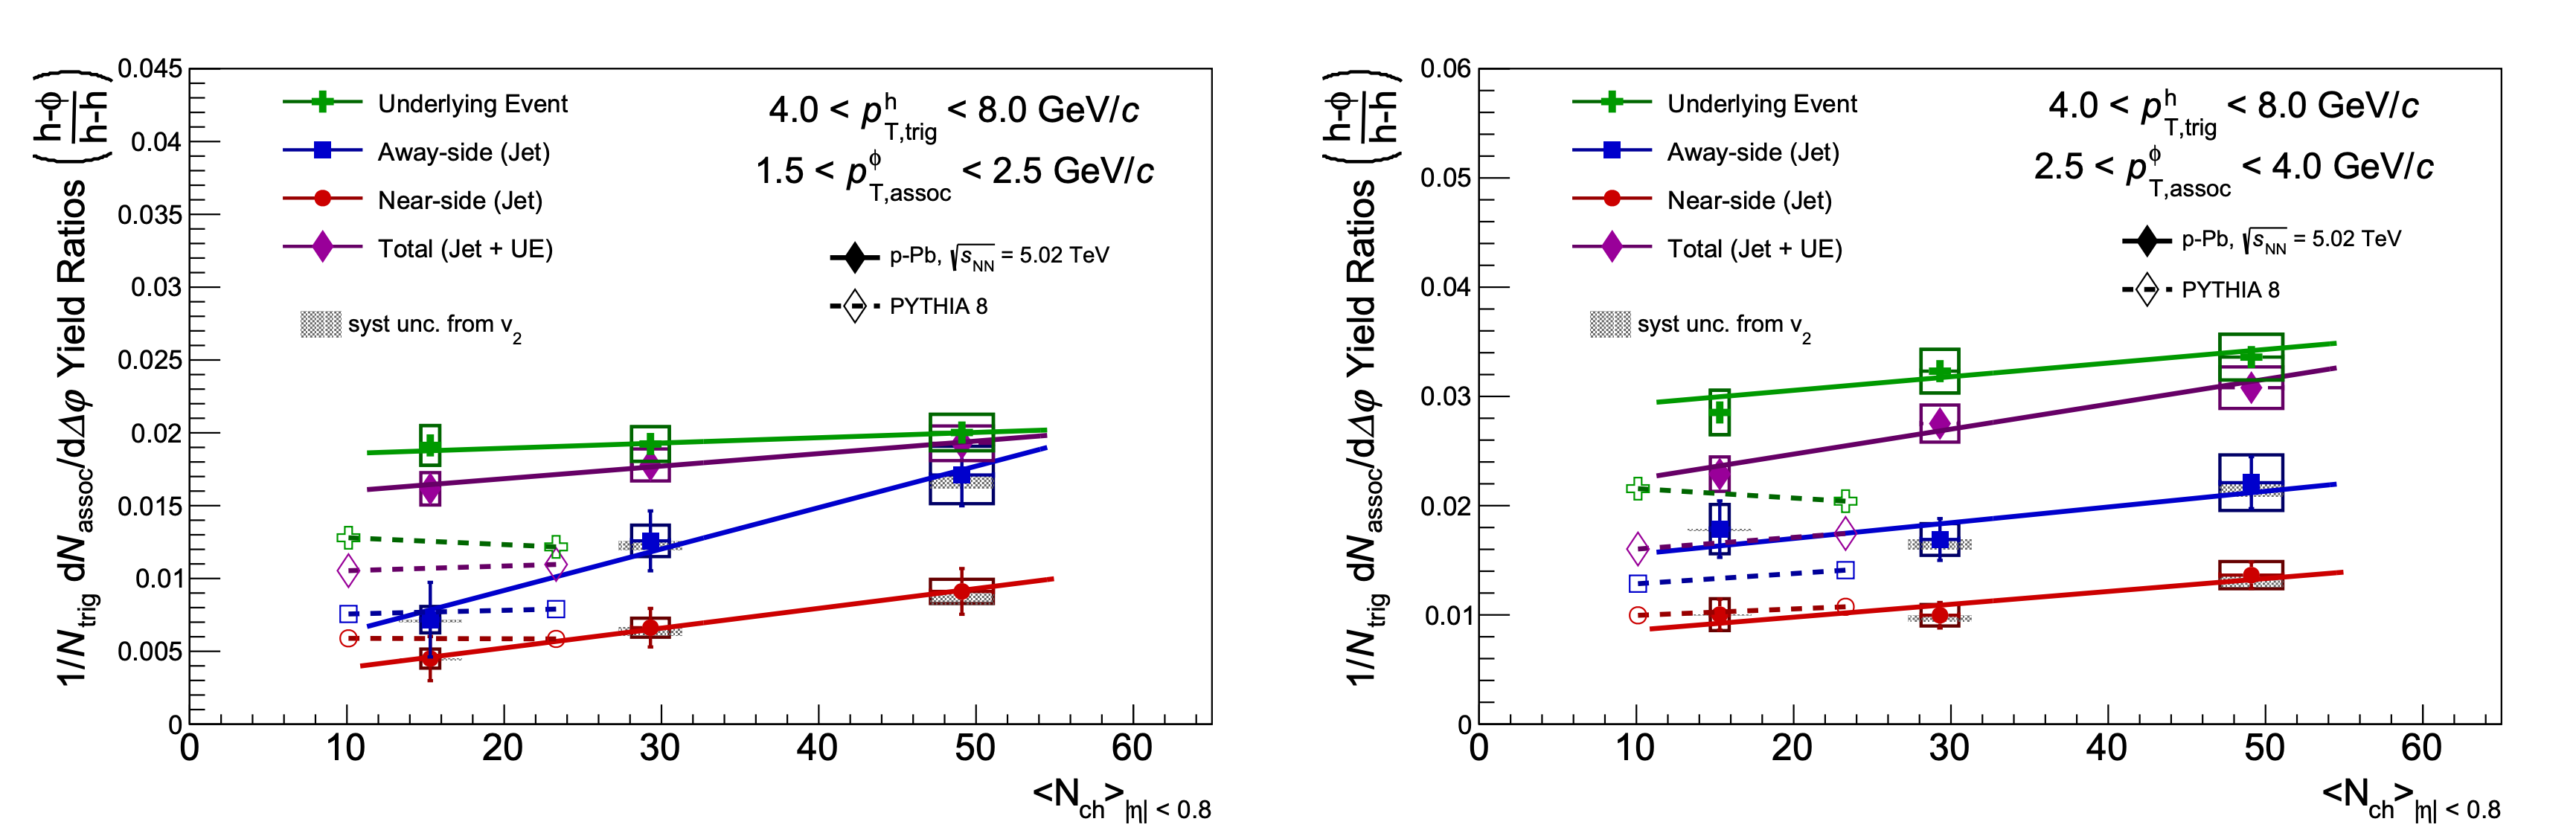
\includegraphics[width=\textwidth]{figures/results/justin_plots.png}
\caption{Previously published results for the per-trigger pair-wise yield ratios $R_{i}^{\phi/h} \equiv Y_{i}^{h-\phi}/Y_{i}^{h-h}$ ($i$ = near-side, away-side, UE, total) as a function of charged particle multiplicity for lower (left) and higher (right) associated \pt ranges.}
\label{fig:justin_plots}
\end{figure}

\begin{figure}[h!]
\centering
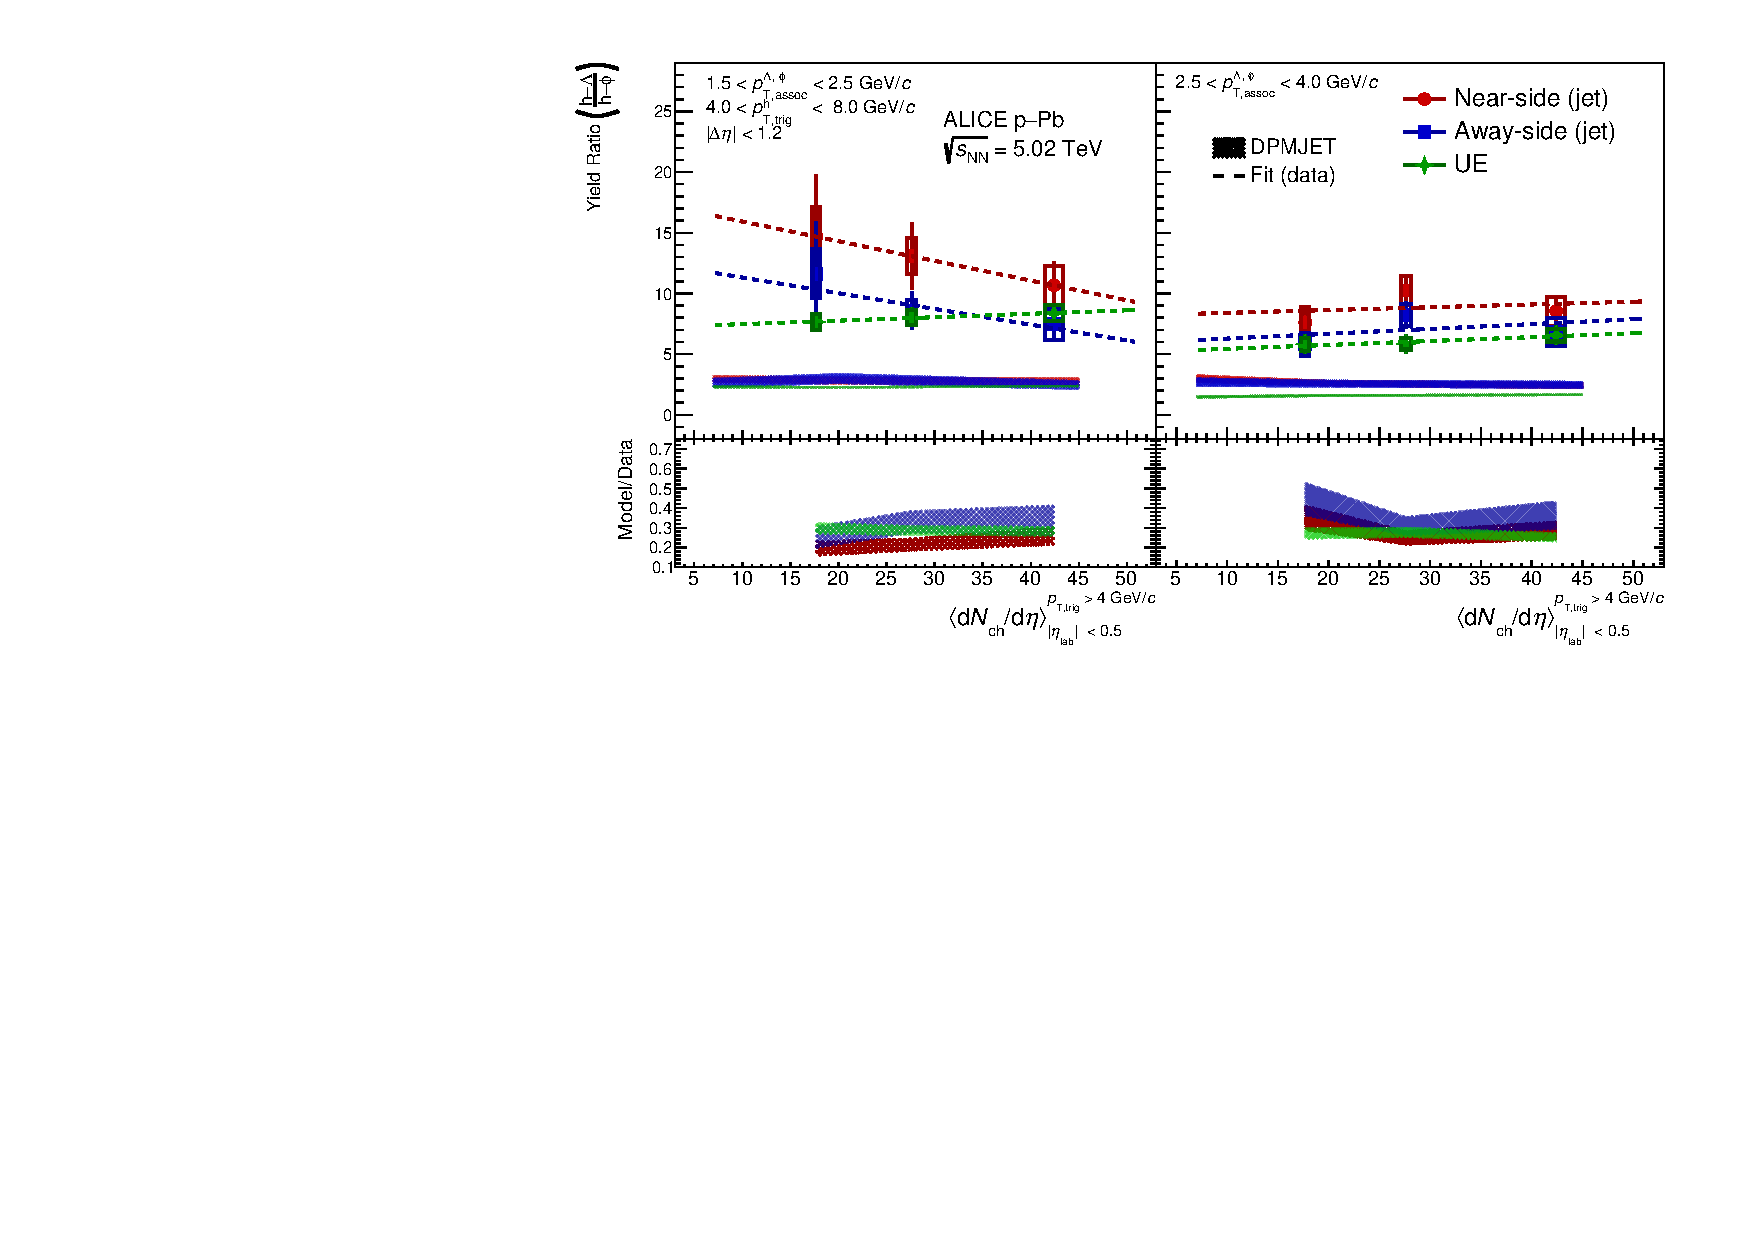
\includegraphics[width=\textwidth]{figures/results/final_lambda_phi_ratio_plot_new_x_axis_model_ratio.pdf}
\caption{The per-trigger pair-wise yield ratios $R_{i}^{\Lambda/\phi} \equiv Y_{i}^{h-\Lambda}$/$Y_{i}^{h-\phi}$ ($i$ = near-side, away-side, UE) as a function of multiplicity in the lower (left) and higher (right) associated momentum ranges. The statistical (systematic) uncertainties are shown as vertical lines (boxes).  The ratios predicted by DPMJET are also presented as shaded bands, with the width of the band represending the systematic uncertainty on the model. The ratio of the model to the data is presented in the bottom panel.}
\label{fig:lambda_phi_ratio}
\end{figure}

Interestingly, $\Lambda/\phi$ near-side ratios are systematically higher than the ratios in all other regions across the entire multiplicity range and both momentum ranges. This indicates relative enhancement (supression) of $\Lambda$ ($\phi$) production along the jet axis. As strangeness is always produced in the form of $s\bar{s}$ pairs, one possible explanation of this effect is that when these pairs are produced from jet fragmentation, the $s$ and $\bar{s}$ are less likely to hadronize into the same $\phi$ due to their separation in phase-space. The away-side ratios are higher than the UE ratios on average, but the difference is not as pronounced as in the near-side.  The ratios predicted by DPMJET provide further evidence for this explanation, as the model shows the near- and away-side ratios are systematically higher than the UE ratios across the entire multiplicity range. However, DPMJET predicts no differences between the near- and away-side $\Lambda$/$\phi$ ratios, possibly due to the missing medium effects in the model. While the central values of the near- and away-side ratios in the lower associated momentum range decrease with increasing multiplicity, the uncertainties are very large. All of the slopes presented in Table \ref{tab:lambda_phi_slopes} are compatible with zero, indicating no dependence on multiplicity for the $\Lambda$/$\phi$ ratios.

\begin{table}
\centering
\caption{The slopes obtained from the straight-line fits to the per-trigger pair-wise (h-$\Lambda$)/(h-$\phi$) yield ratios as a function of multiplicity in both associated momentum ranges. The fits are made using the statistical and systematic errors summed in quadrature. All fits are such that $\chi^{2}/\text{ndf} < 1$.}
\begin{tabular}{l c c}
\hline
Region & Lower $p_{\text{T, assoc}}^{\Lambda, \phi}$ slope ($\times10^{-1}$) & Higher $p_{\text{T, assoc}}^{\Lambda, \phi}$ slope ($\times10^{-1}$) \\
\hline
Near-side & $ -1.6\pm 2.0$ & $0.2 \pm 0.9$ \\
Away-side & $ -1.1 \pm 1.4$ & $0.3 \pm 0.7$ \\
UE & $0.3 \pm 0.4$ & $0.3 \pm 0.3$ \\
\hline
\end{tabular}
\label{tab:lambda_phi_slopes}
\end{table}

The near- and away-side slopes reported in Table \ref{tab:lambda_hadron_slopes} are all more than $2\sigma$ greater than zero, indicating that there is an enhancement of relative $\Lambda$ production in jets as a function of multiplicity. This result is consistent with previous measurements of the $\phi(1020)$ meson in jets ~\cite{JustinPaper}, where a similar enhancement of the $\phi$/h ratio is observed in the near- and away-side regions. This provides further evidence that the production of strange quarks is enhanced in jets. The away-side slopes are also systematically larger than the near-side slopes in both momentum ranges, again hinting at possible modification of the away-side $s$-quark production due to jet-medium interactions. Similarly, the UE slopes are not compatible with zero, but the value is smaller than the near- and away-side slopes by about $1\sigma$ in the lower momentum range. However, the larger values of the UE ratios overall still suggest that a significant portion of the observed enhancement in the $\Lambda$/$\pi$ ratio is due to softer production from the UE. The slopes calculated using the ratios obtained from DPMJET are all nearly exactly zero, and are thus not shown in the table.